\chapter{Modeling the effects of cyclic loading on exogenously crosslinked tissues}

\section*{Preface}
\addcontentsline{toc}{section}{Preface}%

    Bioprosthetic heart valves (BHVs), fabricated from exogenously crosslinked collagenous tissues, remain the most popular heart valve replacement design. However, the life span of BHVs remains limited to 10-15 years, in part because the mechanisms that underlie BHV failure remain poorly understood. Experimental evidence indicates that BHVs undergo significant changes in geometry with \textit{in vivo} operation, which leads to stress concentrations that can have significant impact on structural damage. These changes do not appear to be due to plastic deformation, as the leaflets only deform in the elastic regime. Moreover, structural damage was not detected by the 65 million cycle time point. Instead, we found that this nonrecoverable deformation is similar to the permanent set effect observed in elastomers, which allows the reference configuration of the material to evolve over time. We hypothesize that the scission-healing reaction of glutaraldehyde is the underlying mechanism responsible for permanent set in exogenously crosslinked soft tissues. The continuous scission-healing process of glutaraldehyde allows a portion of the exogenously crosslinked matrix, which is considered to be the non-fibrous part of the extra-cellular matrix, to be re-crosslinked in the loaded state. Thus, this mechanism for permanent set can be used to explain the time evolving mechanical response and geometry of BHVs in the early stage. To model the permanent set effect, we assume that the exogenously crosslinked matrix undergoes changes in reference configurations over time. The changes in the collagen fiber architecture due to dimensional changes allow us to predict subsequent changes in mechanical response. Results show that permanent set alone can explain and, more importantly, predict how the mechanical response of the biomaterial change with time. Furthermore, we found is no difference in permanent set rate constants between the strain controlled and the stress controlled cyclic loading studies. An important finding we have is that the collagen fiber architecture has a limiting effect on the maximum changes in geometry that the permanent set effect can induce. This is due to the recruitment of collagen fibers as the changes in geometry due to permanent set increases. This means we can potentially optimize the BHV geometry based on the predicted the final BHV geometry after permanent set has largely ceased. Thus, we have developed the first structural constitutive model for the permanent set effect in exogenously crosslinked soft tissue, which can help to simulate BHV designs and reduce changes in BHV geometry during cyclic loading and thus potentially increasing BHV durability.
    
\textbf{The work contained in this chapter was published as}: Zhang, W. \& Sacks, M. S.
Modeling the response of exogenously crosslinked tissue to cyclic loading: The effects of permanent set. 
Journal of the mechanical behavior of biomedical materials, 2017, 75, 336-350 




%---    INTRODUCTION
%%%%%%%%%%%%%%%%%%%%%%%%%%%%%%%%%%%%%%%%%%%%%%%%%%%%%%%%%%%%%%%%%%%%%%%%%%%%%%%%
%% Introductions
%%%%%%%%%%%%%%%%%%%%%%%%%%%%%%%%%%%%%%%%%%%%%%%%%%%%%%%%%%%%%%%%%%%%%%%%%%%%%%%%


\section{Introduction}

%%%%%%%%%%%%%%%%%%%%%%%%%%%%%%%%%%%%%%%%%%%%%%%%%%%%%%%%%%%%%%%%%%%%%%%%%%%%%%%%
%%%%    Background

\subsection{Background and clinical significance}

	Heart valve treatment is a common cardiovascular surgical procedure with over 100,800 done annually in the U.S. alone \cite{mozaffarian_heart_2016} and 275,000 to 370,000 in developed nations \cite{manji_future_2012}. Almost all contemporary heart valve replacement designs use exogenously crosslinked (EXL) collagenous soft tissues (e.g. bovine pericardium) to manufacture leaflets for bioprosthetic valves (BHVs) \cite{starr_artificial_2007, soares_biomechanical_2016}. BHVs have advantages in immunogenicity and hemodynamics over other designs, but also have a limited life span of 10-15 years. As a recent development in BHV technology, transcatheter valve interventions \cite{bonow_accaha_2006, guidoin_marvel_2010} reduce surgical risk and make valve replacement more feasible for those who cannot tolerate full surgical interventions. However, this new technology also presents additional design challenges, including complex folding and compression during delivery. As a result, the leaflets are required to be significantly thinner than in traditional BHVs, which increases the leaflet stress and potentially the rate of failure. Existing data on transcatheter aortic valve interventions suggest a 2-year mortality rate of 33.9\% overall \cite{mozaffarian_heart_2016} and over 68\% when specifically replacing stenotic aortic valves \cite{makkar_transcatheter_2012}. As such, this further accentuates the need to develop an approach to improve BHV durability. 
	
%%%%%%%%%%%%%%%%%%%%%%%%%%%%%%%%%%%%%%%%%%%%%%%%%%%%%%%%%%%%%%%%%%%%%%%%%%%%%%%%
%%%%    Failure
	 
\subsection{Mechanisms of BHV failure}

	The causes of BHV failure can be divided into two broad categories, mineralization and structural damage, with both processes occurring in parallel or independently \cite{sacks_collagen_2002}. Mineralization is the accumulation of mineral deposits, mainly calcium phosphate, within the BHV leaflets \cite{schoen_calcification_2005}. This disrupts the underlying microstructure preventing the proper mechanical function of BHVs, increasing the likelihood of tearing, and reducing flexibility (preventing normal opening and closing motions, and induce valve stenosis). This process is exacerbated by the presence of exogenous crosslinkers, such as glutaraldehyde (GLUT), where the phosphates from the devitalized endothelial cells bind with the calcium in blood to form deposits. The causes of calcification and associated anti-calcification treatments are extensively studied in literature \cite{park_novel_1997, isenburg_tannic_2005, vyavahare_prevention_1997}. On the other hand, structural damage includes the collagen fiber damage and breakdown of the non-fibrous part of extracellular matrix (ECM), \emph{which we will refer as simply the matrix}. Fourier transform infrared spectroscopy(FTIR) results have shown changes in the collagen fiber molecular structure after 50 million cycles \cite{sun_response_2004}, which suggests that some collagen fiber damage has occurred during this period. However, its effect on the mechanical response of BHVs was not detectable. Nevertheless, it is important to maintain the structural integrity of the BHV, as this will help to improve BHV durability. 
	
%%%%%%%%%%%%%%%%%%%%%%%%%%%%%%%%%%%%%%%%%%%%%%%%%%%%%%%%%%%%%%%%%%%%%%%%%%%%%%%%
%%%%    Cyclic loading
	
\subsection{Response to long-term cyclic loading}

	The current process for evaluating BHV designs is an expensive and time consuming three-stage process: 1) accelerated wear testing(AWT), 2) large animal studies, and 3) clinical trials. AWT is performed by cycling BHVs in sterile saline at 10 to 20 times the normal heart rate. It is currently the only way to evaluate BHV durability in a feasible amount of time (months instead of years). However, the loading conditions and environment during AWT are not physiological and the only durability information currently used is the presence of visible damage. Designs which show promise are then put through costly large animal studies, which still do not fully duplicate the human native environment. The final and most important stage is clinical evaluations. This is the only stage in evaluation process that can provide true indications of the \textit{in vivo} performance of BHV designs. However, this is the final, most difficult, most expensive and most time consuming stage. Clearly, current methods of evaluating BHV designs are not feasible for advancing the BHV technology in a timely manner. Computational simulations have been presented as an effective approach to this problem\cite{soares_biomechanical_2016}. To be effective, we need better a understanding of the underlying mechanisms of structural damage. 
	

	However, these mechanisms are poorly understood, especially for how they affect the mechanical response of the exogenously crosslinked tissues used to construct the BHV leaflets. The most significant change in response to cyclic loading is the change in geometry of the BHV leaflets. In a study on the porcine aortic BHVs \cite{smith_high_1997},  Smith \textit{et al}. found significant changes in the unloaded geometry of BHVs after AWT, especially in the belly region of the leaflets (Fig. \ref{fig:PSeffects}A). By changing the unloaded reference configuration, the shape of the leaflets and their mechanical response will change as well. Further analysis shown that significant structure damage occurred within the belly region as compared to other regions of the leaflet, where the stress significantly increased \cite{smith_fatigue_1999}. Interestingly, Smith et al. also found most the most significant changes in BHV leaflet geometry to occur within first 50 million cycles \cite{smith_high_1997}. Moreover, Sacks and Smith \cite{sacks_effects_1998} also found that there were minimal structural damage in this early stage (Fig. \ref{fig:PSeffects}B). This is further supported by another study by Wells \textit{et al} \cite{wells_cyclic_2005}, where they found minimal structural changes during the first 50 million cycles for the pressure fixed BHVs, with most significant change observed in the first million cycles. Clearly, there is a non-damage based mechanism at play that changes the geometry of the material, with significant impact on the early stage of cycling and the rate of fatigue in later stages. 


\begin{figure}[hbt]
\centering
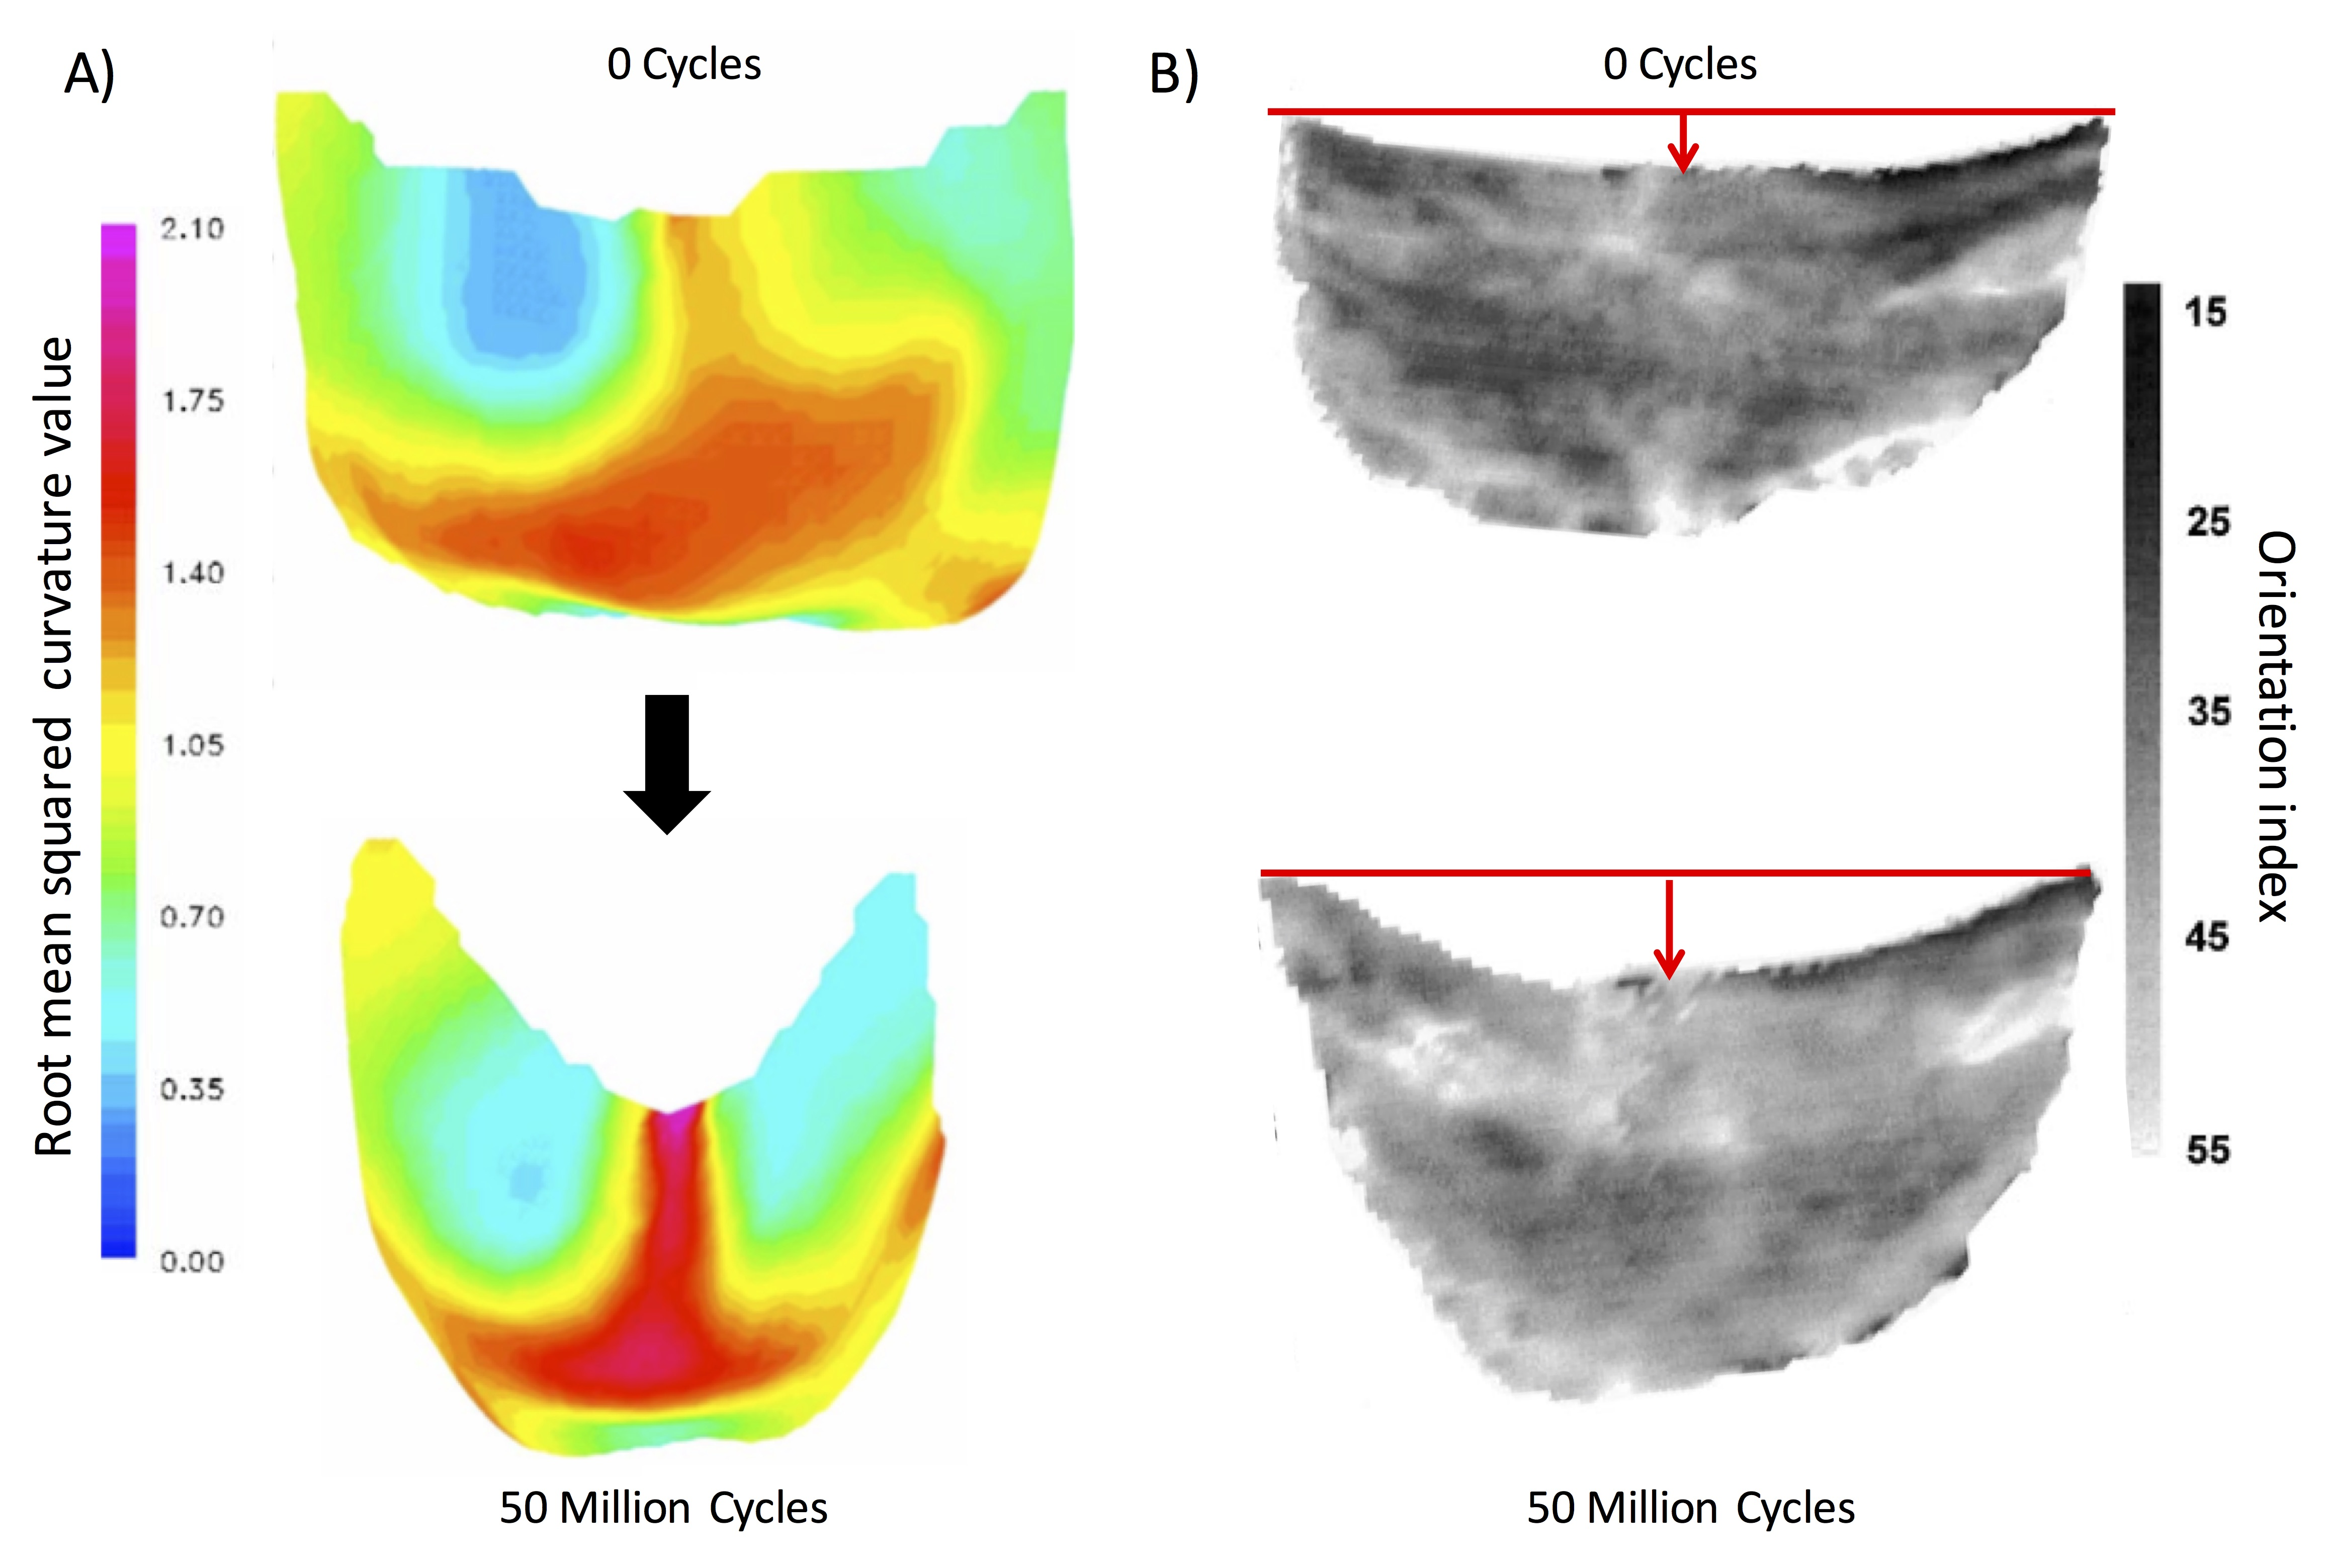
\includegraphics[width=\textwidth]{Images/chapter4/figure1}
\caption{A) The 3D unloaded geometry a BHV leaflet before and after cyclic loading, with the color indicating the local root mean squared curvature. The most significant change in geometry is in the belly region. B) BHV leaflet collagen fiber architecture, showing that the collagen fiber architecture are convected by the dimensional changes. The grayscale scale bar shows the orientation index (OI), which is angle containing 50 \% of fibers. The lack of changes in the OI suggests that minimal damage to the collagen fiber architecture has occurred.}
\label{fig:PSeffects}
\end{figure}


%%%%%%%%%%%%%%%%%%%%%%%%%%%%%%%%%%%%%%%%%%%%%%%%%%%%%%%%%%%%%%%%%%%%%%%%%%%%%%%%
%%%%    Exogenous crosslinking

\subsection{The effect of exogenous crosslinking}

	Bovine pericardium (BP) is a dense collagenous tissue composed mostly of collagen type I fibers with some elastin, GAGs, cells and vasculature. Collagen fibers are complex protein structures at the 2 - 10 $\mu$m scale, composed of tightly bundled collagen fibrils, which are approximately 50 nm in diameter. Much of what we know about the use of GLUT to exogenously crosslink collagenous tissue is from Nimni \textit{et al.} \cite{cheung_mechanism_1990, nimni_chemically_1987, cheung_mechanism_1985, gendler_toxic_1984, cheung_presence_1983, cheung_mechanism_1982, cheung_mechanism_1982II}. GLUT, which is an aldehyde based crosslinker, aggressively crosslinks free amines in proteins. This suppresses immunogenicity by crosslinking all cell membrane protein remnants, but also forms polymeric networks (at the nm scale) which allow for long range crosslinks to the nearby tissue microstructures. We previously found that exogenous crosslinking increases the bending stiffness of the matrix by four time the original stiffness \cite{mirnajafi_effects_2010}. We also tested the mechanical response of exogenously crosslinked BP before and after crosslinking, and developed the first constitutive model for exogenously crosslinked soft tissue \cite{sacks_novel_2016}. Interestingly, we also found that exogenously crosslinking does not increase the collagen fiber modulus, but significantly increases the interactions between collagen fibers \cite{sacks_novel_2016}, which is responsible for up to 30\% of the stress in the fully loaded state. 


	The GLUT crosslinking process involves a Schiff-base reaction. Importantly, the molecular bonds formed from Schiff-base reactions are known to be unstable at room and temperatures \cite{migneault_glutaraldehyde_2004, damink_glutaraldehyde_1995}. Thus, although GLUT is highly reactive and aggressively crosslinks extracellular matrix proteins, any resulting crosslinks will also readily undergo hydrolysis at body temperature \cite{migneault_glutaraldehyde_2004}. As a result, under cyclic loading in-vivo, exogenous ECM crosslinks will constantly break and reform. This continual process will cause the reference configuration to evolve towards the current loaded state. \emph{We thus hypothesize that this scission-healing behavior could be linked to the mechanisms that underlie how the BHV leaflet geometry evolves over time}.
	
	
    This damageless change in the BHV geometry has many similarities to the permanent set (PS) mechanisms observed in elastomers. Permanent set is an irreversible deformation that remains after a structure or material has been subjected to external stresses and then released. It does not involve damage to the constituents of the material, but instead changes the referential configuration. Although the outcomes may be similar, \emph{this form of permanent set is not a plastic deformations}, as they are entirely within the elastic regime. In particular, it has been used to model the scission-healing reactions of elastomers that occur when stretched, heated, cooled, then unloaded. This results in some of the materials to change in referential configuration to the loaded state. In this process, permanent set does not damage the polymeric fibers but is a result of the change in configuration of the underlying polymeric fiber network. Some works on constitutive models of this process include the works of Rajagopal and Wineman \cite{rajagopal_constitutive_1992}, Andrews and Tobolsky \cite{andrews_theory_1946}, and Rottach \textit{et al}. \cite{rottach_effect_2004, rottach_molecular_2007, rottach_permanent_2006}. However, there are little known studies on the permanent set effect in soft tissues or soft tissue derived exogenously crosslinked biomaterials. 
	

	\emph{Based on the above considerations, we hypothesize that the initial time evolving BHV geometry and mechanical response can be predicted by permanent set mechanisms}. Rather than heating and cooling, we assume that permanent set in exogenously crosslinked tissue occurs continuously at body temperature due to the GLUT, allowing the reference configuration of the exogenously crosslinked matrix (EXL matrix) to evolve over time. As a result, the reference configuration of BHVs will change while not affecting the intrinsic material properties of their constituents such as collagen fibers and the EXL matrix. Since the BHVs deform into a new configuration (Fig. \ref{fig:PSeffects}), there may develop regions of stress concentrations. The high stresses will increase the rate of structural damage and thus accelerate the rate of BHV failure. Thus, \emph{by compensating for the permanent set effects, it may be possible to reduce the BHV leaflet stresses and thus reduce structural damage to BHVs during \textit{in vivo} operation after implant.} Therefore, constitutive models that can predict the effects of permanent set are crucial for the simulation of BHVs. 

		
%%%%%%%%%%%%%%%%%%%%%%%%%%%%%%%%%%%%%%%%%%%%%%%%%%%%%%%%%%%%%%%%%%%%%%%%%%%%%%%%
%%%%    Constitutive models

\subsection{Constitutive models for the permanent set effect for soft tissues}

	The only work in the simulation of the permanent set effect in native or exogenously crosslinked soft tissues is the pioneering study of Martin and Sun \cite{martin_modeling_2013}, who developed a time dependent constitutive model for uniaxial cyclic loading of GLUT exogenously crosslinked BP strips using a damage analog. Briefly, to model the uncycled mechanical response, they used the Fung hyperelastic model for the strain energy density function, $\Psi_0$. The time dependent stress softening was then described using a modification to the strain energy function as $\Psi_\mathrm{PS} = (1-D_s)\Psi_0 - \Psi_0(\mathbf{E}_\mathrm{PS})$. Here the strain energy of the material after permanent set ($\Psi_\mathrm{PS}$) is reduced from $\Psi_0$ in accordance with a scaled damage function $D_s$ and the same strain energy function evaluated at the current amount of permanent set ($\mathbf{E}_\mathrm{PS}$). Martin and Sun then measured the maximum permanent set deformation that occurs for each specimen, and used that to set the maximum bound of $\mathbf{E}_\mathrm{PS}$. Additionally, Martin and Sun set two parameters, a lowerbound below which no permanent set occurs, and an upperbound above which the tissue fails. In the intermediate region, $D_s$ and $\mathbf{E}_\mathrm{PS}$ simply increase linearly with the number of cycles. The number of cycles needed to reach the maximum permanent set deformation was then described using an inverse exponential like function of the maximum strain applied, which is an analogous to the stress versus cycles (S–N) curve used to describe the fatigue behavior of traditional engineering materials. However, such approaches have the following limitations: 1) they are not predictive as there are no underlying mechanisms in the model. A damage-like model can mimic the results of permanent set but cannot explain nor predict the mechanisms responsible in exogenously crosslinked tissue, and 2) there is no way to extrapolate for predicting into unmeasured regimes using the Fung hyperelastic model. Therefore, there is a need for a more predictive constitutive model that utilizes the underlying mechanisms.


%%%%%%%%%%%%%%%%%%%%%%%%%%%%%%%%%%%%%%%%%%%%%%%%%%%%%%%%%%%%%%%%%%%%%%%%%%%%%%%%
%%%%    A new approach

\subsection{A new approach for modeling the permanent set effect in exogenously crosslinked soft tissues}

	We utilize a structural constitutive modeling approach, which integrates information on tissue composition and structure for material characterization \cite{sacks_structural_2000}. In principal, using structural models we only need to perform parameter estimation for the intrinsic material properties, such as collagen fiber modulus and EXL matrix modulus, to predict the mechanical response using the quantified tissue microstructure. This mechanism based approach allows us to predict the mechanical response at strains outside of the strain range of the experimental data used for parameter estimation \cite{zhang_meso_2016, fata_insights_2014}; a feat not possible using purely phenomenological approaches. In addition, by using a structural modeling approach coupled with the permanent set mechanism to predict the collagen fiber architecture after cyclic loading, we can also predict the mechanical response of the soft tissue at higher cycle numbers. Thus, we use 1) the structural model parameters obtained in the uncycled mechanical state and 2) the permanent set mechanisms to predict how the mechanical response of the exogenously crosslinked tissues evolves with cyclic loading. The key aspects of our approach include:
\begin{enumerate}
\item Model the change in mechanical response entirely as a kinematic change in the underlying microstructure; no actual change in mechanical properties (damage)
\item Predict the change in geometry from the loading history and the permanent set mechanism
\item Validate the permanent set mechanism under both strain and stress controlled loading conditions
\item Develop a time dependent implementation with an evolving loaded configuration under stress control
\end{enumerate}

%---    Experimental methods and data post-processing
%%%%%%%%%%%%%%%%%%%%%%%%%%%%%%%%%%%%%%%%%%%%%%%%%%%%%%%%%%%%%%%%%%%%%%%%%%%%%%%%
%% Overall Approach
%%%%%%%%%%%%%%%%%%%%%%%%%%%%%%%%%%%%%%%%%%%%%%%%%%%%%%%%%%%%%%%%%%%%%%%%%%%%%%%%


\section{Overall modeling approach} \label{sec:modelapproach}

	We hypothesize that permanent set and structural damage are two separate and largely sequential mechanisms that underlie the mechanical response of BHVs. Thus, the life span of BHVs can by separated into three stages: early (up to 2-5 years),  intermediate (up to 10 years), and late stage (up to failure) (Fig. \ref{fig:hypothesis}). In the early stage, permanent set induces significant changes in BHV geometry while structural damage does not play a detectable role. This leads to increased stress and structural damage in the intermediate term which leads to failure in the late term. Thus, by compensating for the effect of permanent set on the geometry, we hypothesize that we can extend the life span of BHVs. We focus our model on the early stage of cyclic loading and build a solid foundation for modeling and simulating the later stages.


\begin{figure}[hbt]
\centering
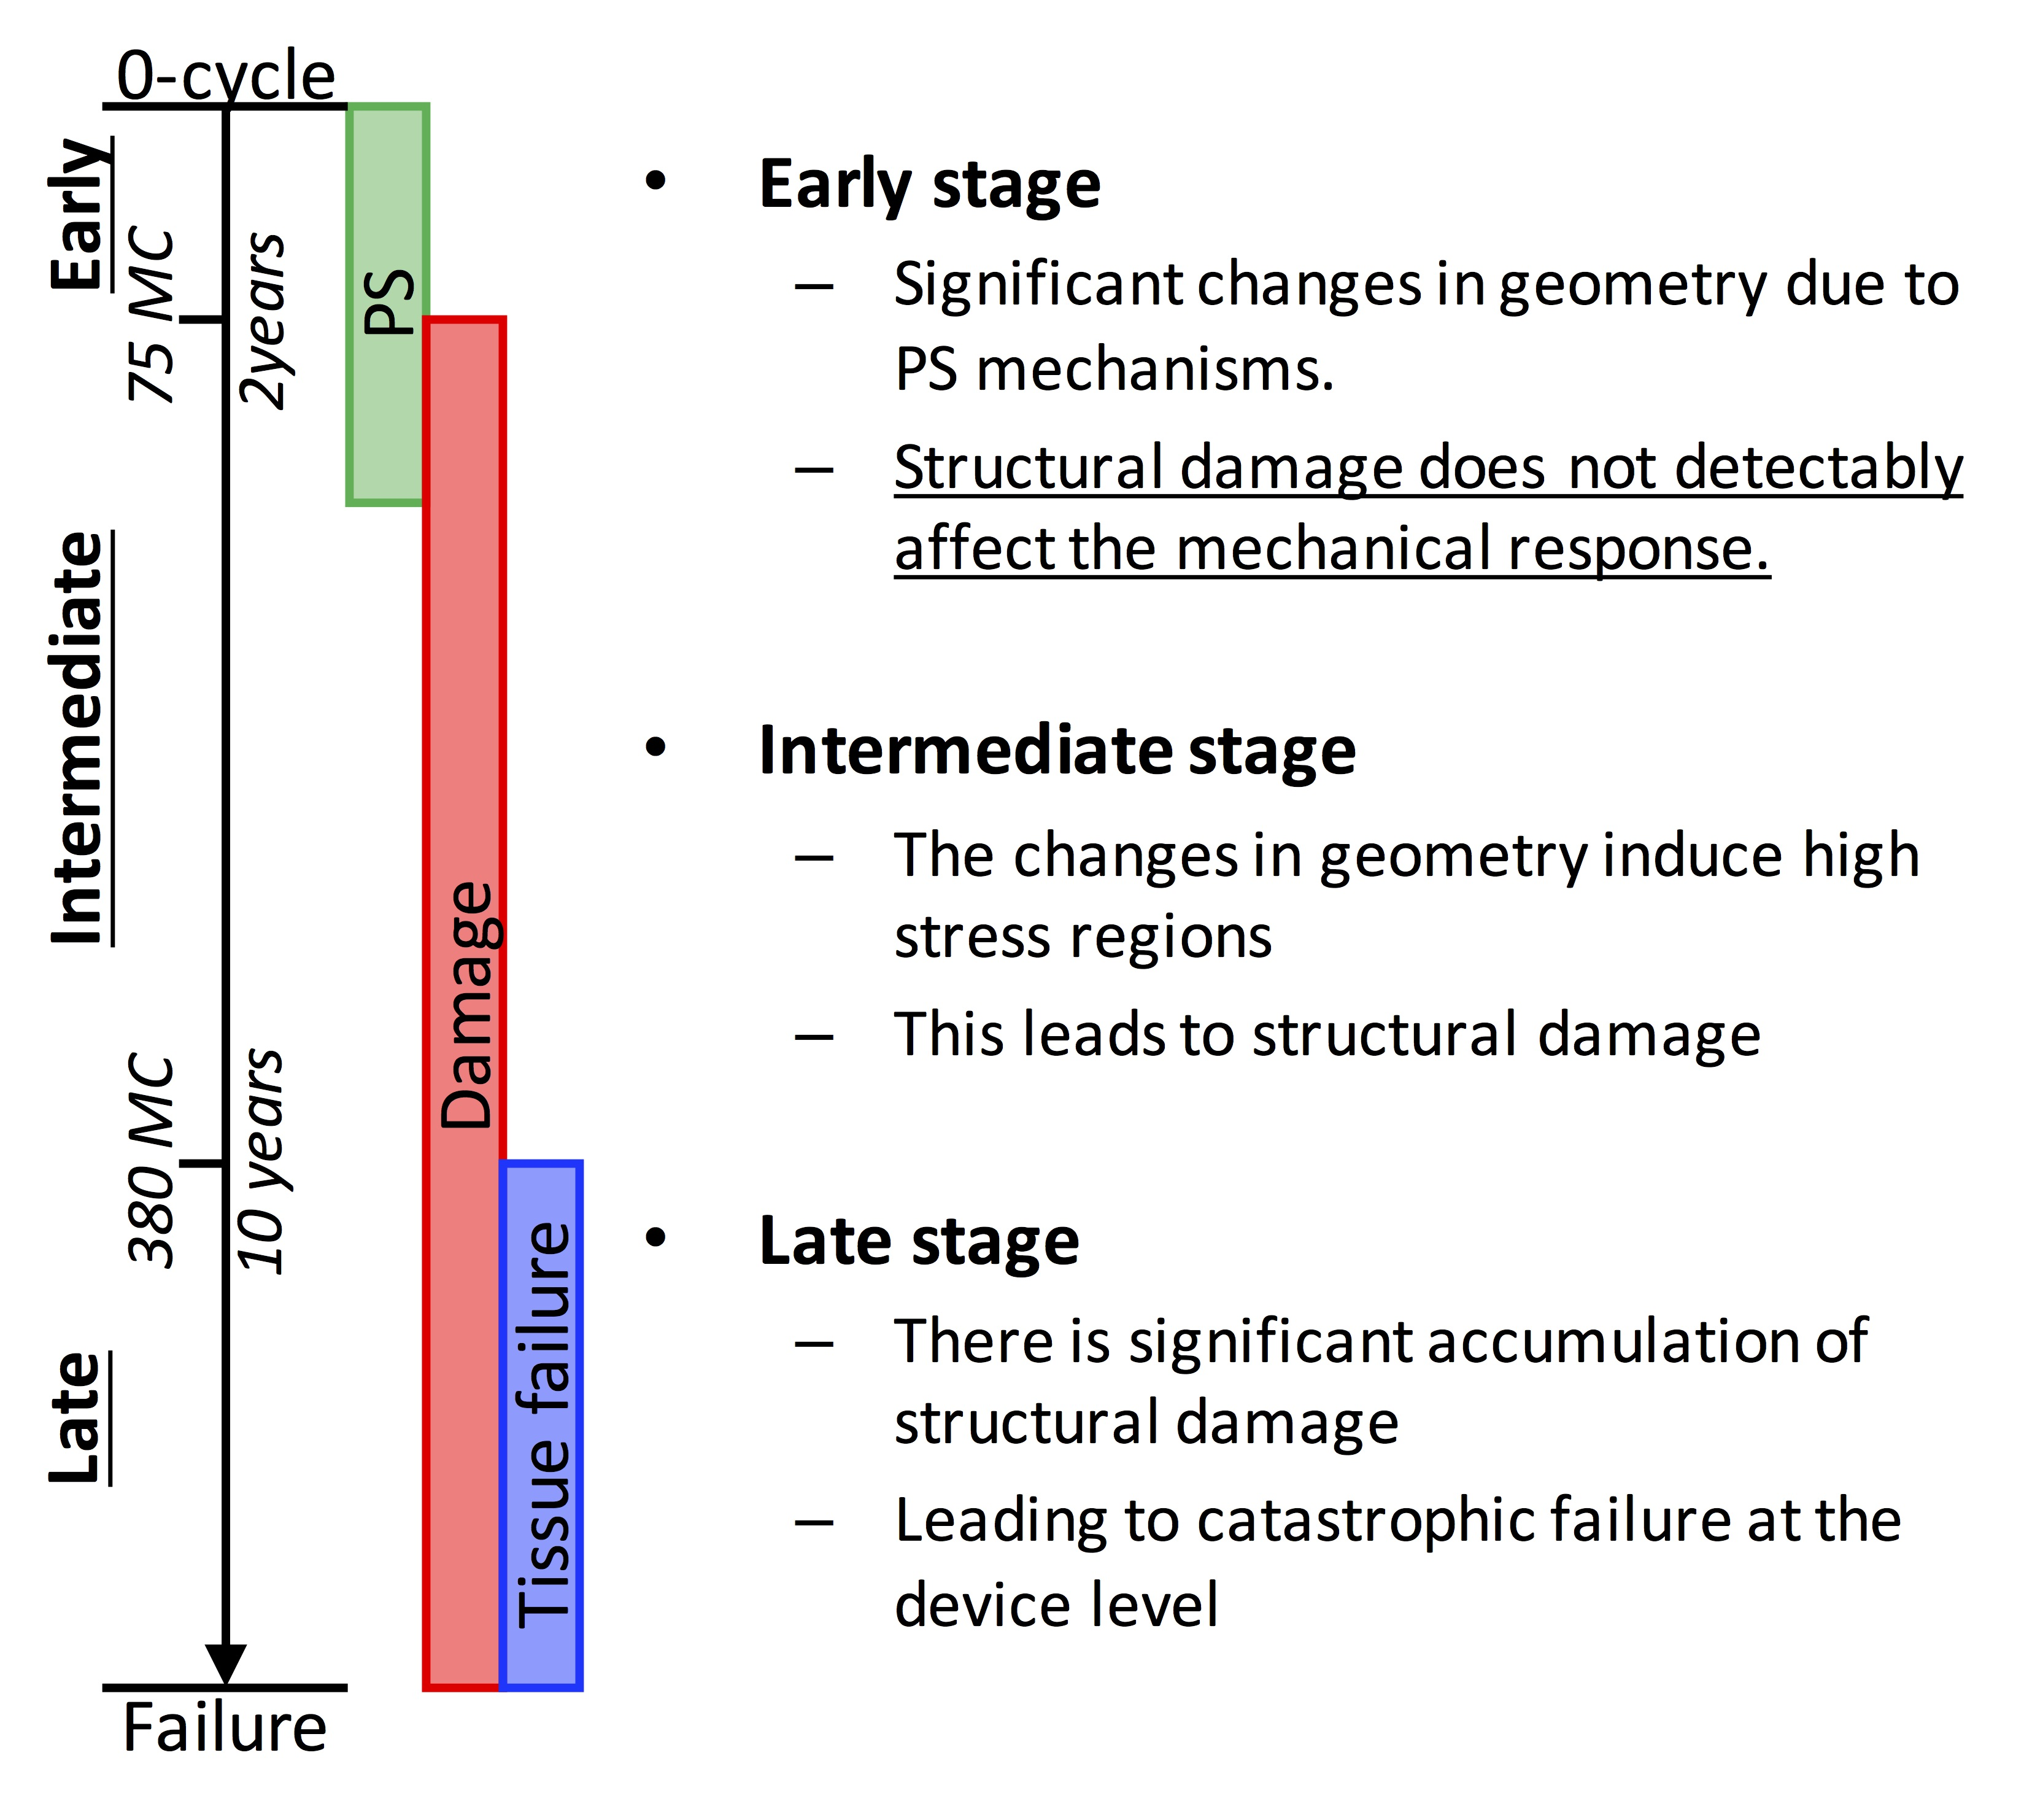
\includegraphics[width=4in]{Images/chapter4/figure2}
\caption{We speculate that the progression of structural damage and permanent set of BHV leaflets progress during long term cyclic loading can be separated into three stages: early, intermediate, and late.}
\label{fig:hypothesis}
\end{figure}


	We assume that permanent set is driven by the scission-healing behaviors of the GLUT polymer network in the non-fibrous EXL matrix, allowing for fractions of it to change in reference state (Fig. \ref{fig:PS}A). The formation of aldehyde bonds during crosslinking, as well as the occasional hydrolysis of the aldehyde bonds follows \emph{first order molecular kinetics} \cite{migneault_glutaraldehyde_2004}. Since this process drives the scission-healing of GLUT polymers and thus permanent set, we hypothesize that permanent set also follows first order kinetics. In addition, we note that the length scale of crosslinks formed by GLUT polymers ($\mathrm{nm}$) in the EXL matrix is several orders of magnitude smaller than that of the collagen fibers ($\mu \mathrm{m}$). Thus, we assume that the collagen fiber architecture does \emph{not} undergo scission-healing like the EXL matrix. Instead, the collagen fibers remain intact during cyclic loading. Rather, the collagen fiber architecture is convected by the changes in geometry that occurs with permanent set in the EXL matrix (Fig. \ref{fig:PS}B). \emph{We refer to this mechanism as structural convection, which is defined as applying a permanent deformation (elongation and rotation of collagen fibers, Fig. \ref{fig:structuralconvection}) to the collagen fiber architecture based on the change in the reference configuration}. Previously, we have shown that dense collagenous tissues deform under affine kinematics \cite{lee_presence_2015}. Since deformations during cyclic loading are in the elastic regime and cyclic loading (second) is on a time scale much shorter than that of permanent set (weeks), the only change in collagen fiber architecture on a cycle to cycle period is also under affine kinematics. Therefore, we also assume that the convection of collagen fiber architecture due to permanent set is under affine kinematics as well. Thus, our approach is based on using the permanent set effect to model the evolving properties of the EXL matrix, determine the change in reference configuration and convect collagen fiber architecture, which then allows us to determine the change in mechanical response of the collagen fibers using structural models. 


\begin{figure}[hbt]
\centering
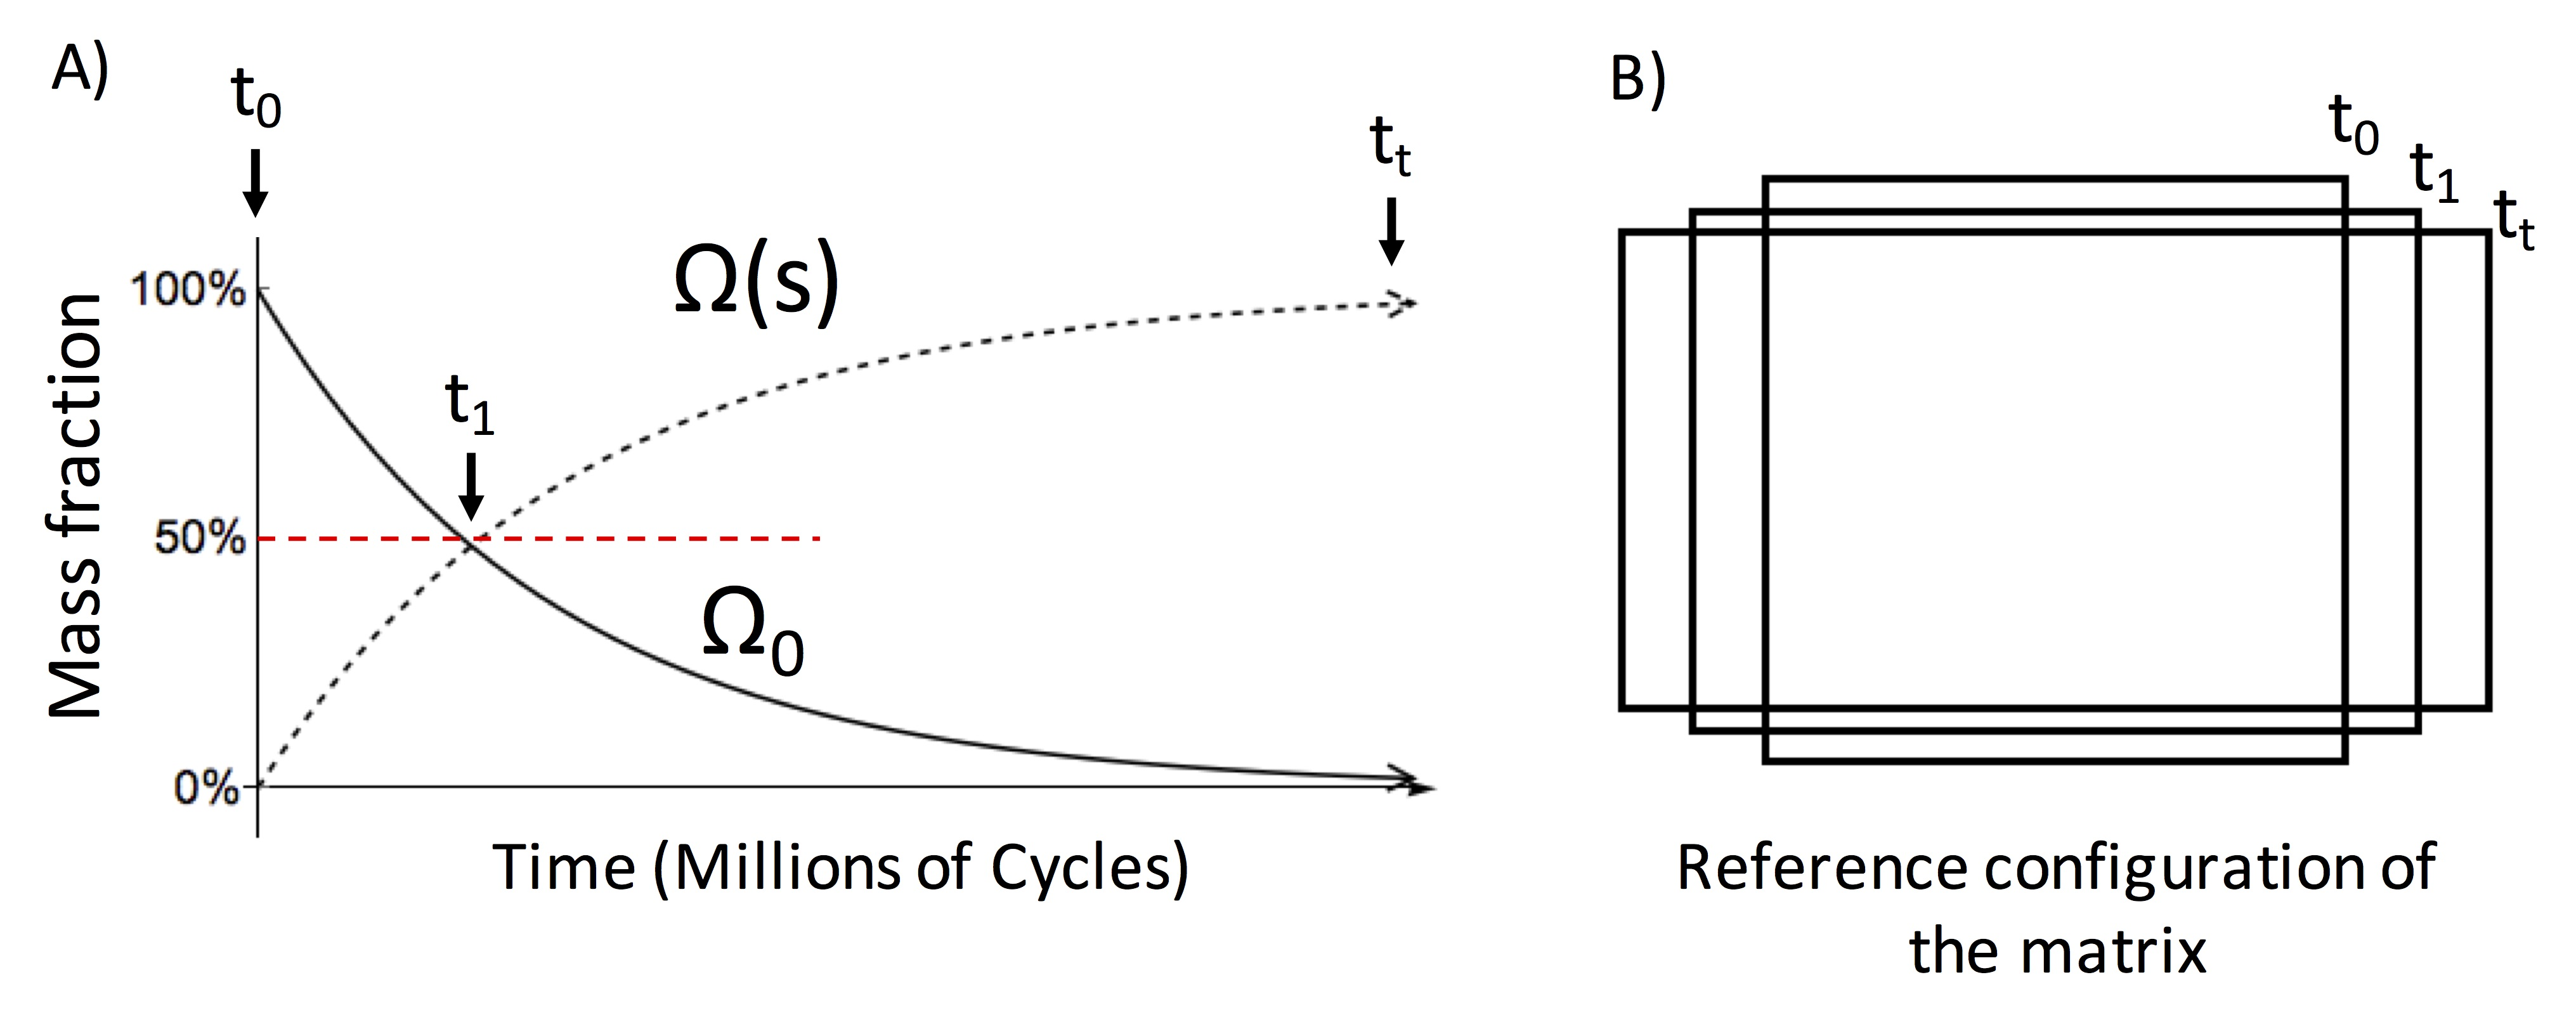
\includegraphics[width=\textwidth]{Images/chapter4/figure3}
\caption{Illustration of the permanent set effect under cyclic uniaxial loading. A) There is a transfer of mass fraction of the EXL matrix to the loaded configuration $\Omega(s)$ from the original state $\Omega_0$. B) This results in changes in the unloaded geometry of the tissue.}
\label{fig:PS}
\end{figure}

\begin{figure}[hbt]
\centering
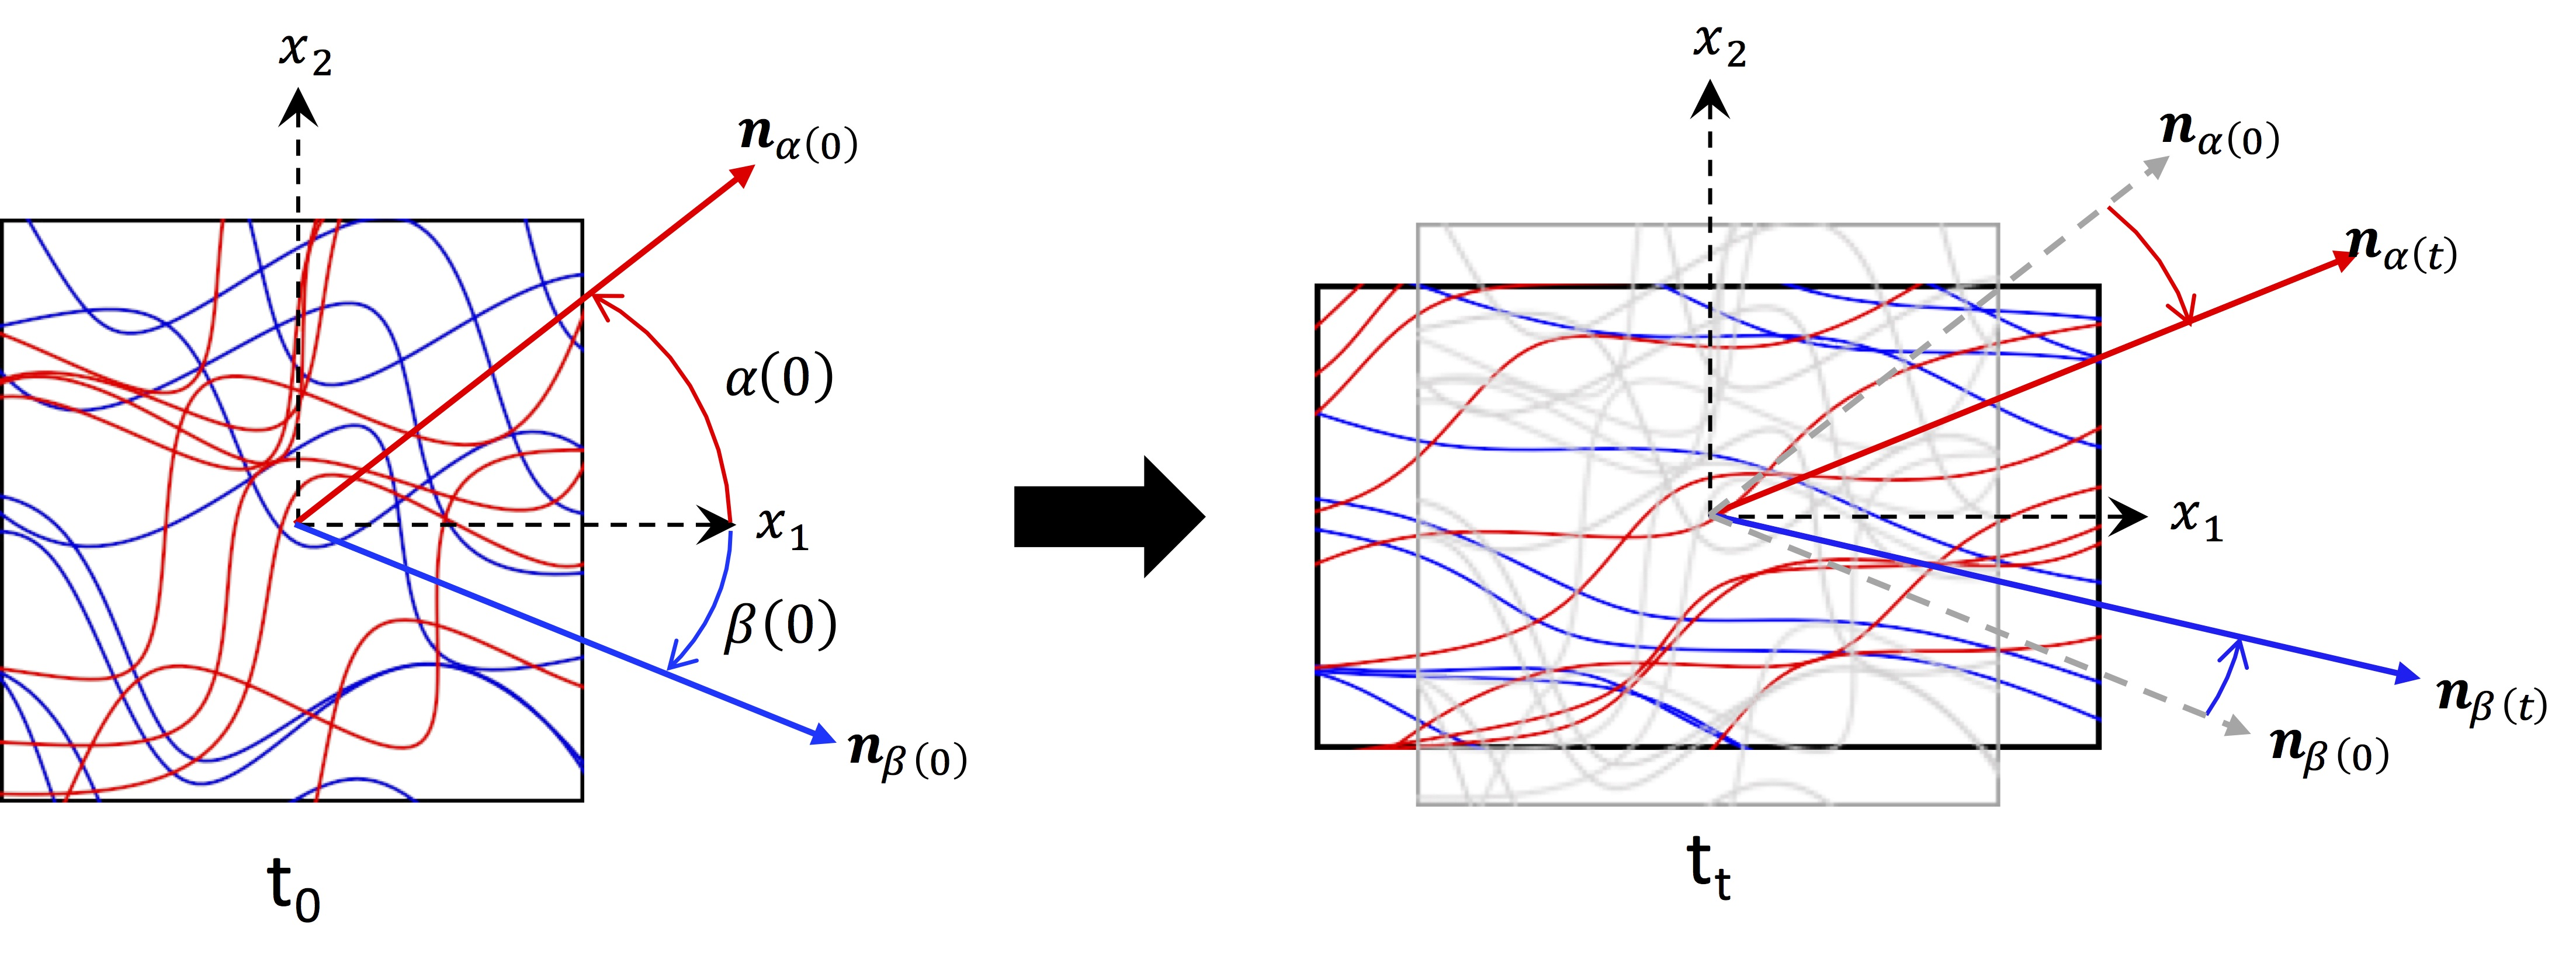
\includegraphics[width=\textwidth]{Images/chapter4/figure4}
\caption{An illustration of how the collagen fiber architecture is convected by changes in the dimension of the bulk tissue. The left figure shows the origin geometry of the tissue at $\mathrm{t}_0$ in figure \ref{fig:PS} while the right figure shows the geometry of the tissue at $\mathrm{t}_t$. Structural convection includes the rotation and straightening of the collagen fiber ensembles. }
\label{fig:structuralconvection}
\end{figure}


	To develop the constitutive model form, we start by modeling the exogenously crosslinked tissue under cyclic loading as parts of a mixture of materials with the same properties but different evolving reference states. The reference state of each part of the EXL matrix is updated according the strain history (Fig. \ref{fig:PS}A). The response of each part are then summed together for the bulk-level mechanical response of the EXL matrix. The new bulk level mechanical response is then used to determine the new unloaded state (Fig. \ref{fig:PS}B). The change in the EXL matrix from its uncycled state is then used to convect the collagen fiber architecture(Fig. \ref{fig:structuralconvection}). The new mechanical response of the EXL matrix is summed with the fiber ensemble interactions and collagen fiber response predicted from the new collagen fiber architecture to determine the full tissue-level mechanical response. Thus, how the \emph{collagen fiber architecture (CFA) is convected by the EXL matrix} is crucial to our model. We start developing our constitutive model by 1) modeling and parameter estimation for the native uncycled mechanical response of the exogenously crosslinked tissue. Then 2) develop the model form for the time evolving mechanical response based on the permanent set mechanism and cyclic loading data. The basic assumptions of our models are:
\begin{enumerate}
\item There is no structural damage to the collagen fibers or the EXL matrix
\item The crosslinking process that induce permanent set follows first order kinetics
\item We are only modeling permanent set under physiological conditions and the process is thus isothermal
\item Permanent set occurs in the isotropic EXL matrix, so that its rate constant is directionally independent
\item The permanent set rate constant is strain-level independent in the physiological range
\item Permanent set occurs over a time scale much longer than a single cardiac cycle
\item The tissue is functionally elastic, and thus viscoelastic effects are ignored
\item The convection of the collagen fiber architecture follows affine kinematics
\item collagen fibers do not bare load or interact until they are straightened
\cite{lee_presence_2015}
\end{enumerate}



%---    Delineation and modelling of the tissue-level mechanical effects of exogenous cross-links
%%%%%%%%%%%%%%%%%%%%%%%%%%%%%%%%%%%%%%%%%%%%%%%%%%%%%%%%%%%%%%%%%%%%%%%%%%%%%%%%
%%  Experimental Data
%%%%%%%%%%%%%%%%%%%%%%%%%%%%%%%%%%%%%%%%%%%%%%%%%%%%%%%%%%%%%%%%%%%%%%%%%%%%%%%%


\section{Extant experimental data}
\label{sec:database}

	We utilized data from the following two extant studies, which differ by their loading conditions and specimen orientations. In the study by Sun \textit{et al}.\cite{sun_response_2004}, exogenously crosslinked BP patches were cycled along the preferred collagen fiber direction (PD) at a peak strain of 16\% and maintained for up to 65 million cycles (Fig. \ref{fig:database}A\&B). The reference configurations of the exogenously crosslinked BP were tracked using fiducial markers attached to the center of the specimens\cite{sacks_biaxial_2000}. The mechanical cycling was stopped at 30 and 65 million cycles for mechanical testing with multiple protocols and different loading paths. It was found that there were significant extensions in the direction of loading (7.1\%), PD, and contractions in the cross direction (-7.7\%). In addition, the collagen fiber crimp period increased from 40.6$\mu$m to 45.24$\mu$m which is consistent with the convection of the collagen fiber architecture that would occur as collagen fiber straighten (Fig. \ref{fig:structuralconvection}). The mechanical response also changed accordingly. The compliance in the PD decreased over time while the compliance in the cross direction of the tissue increased. 
	

\begin{figure}[hbt]
\centering
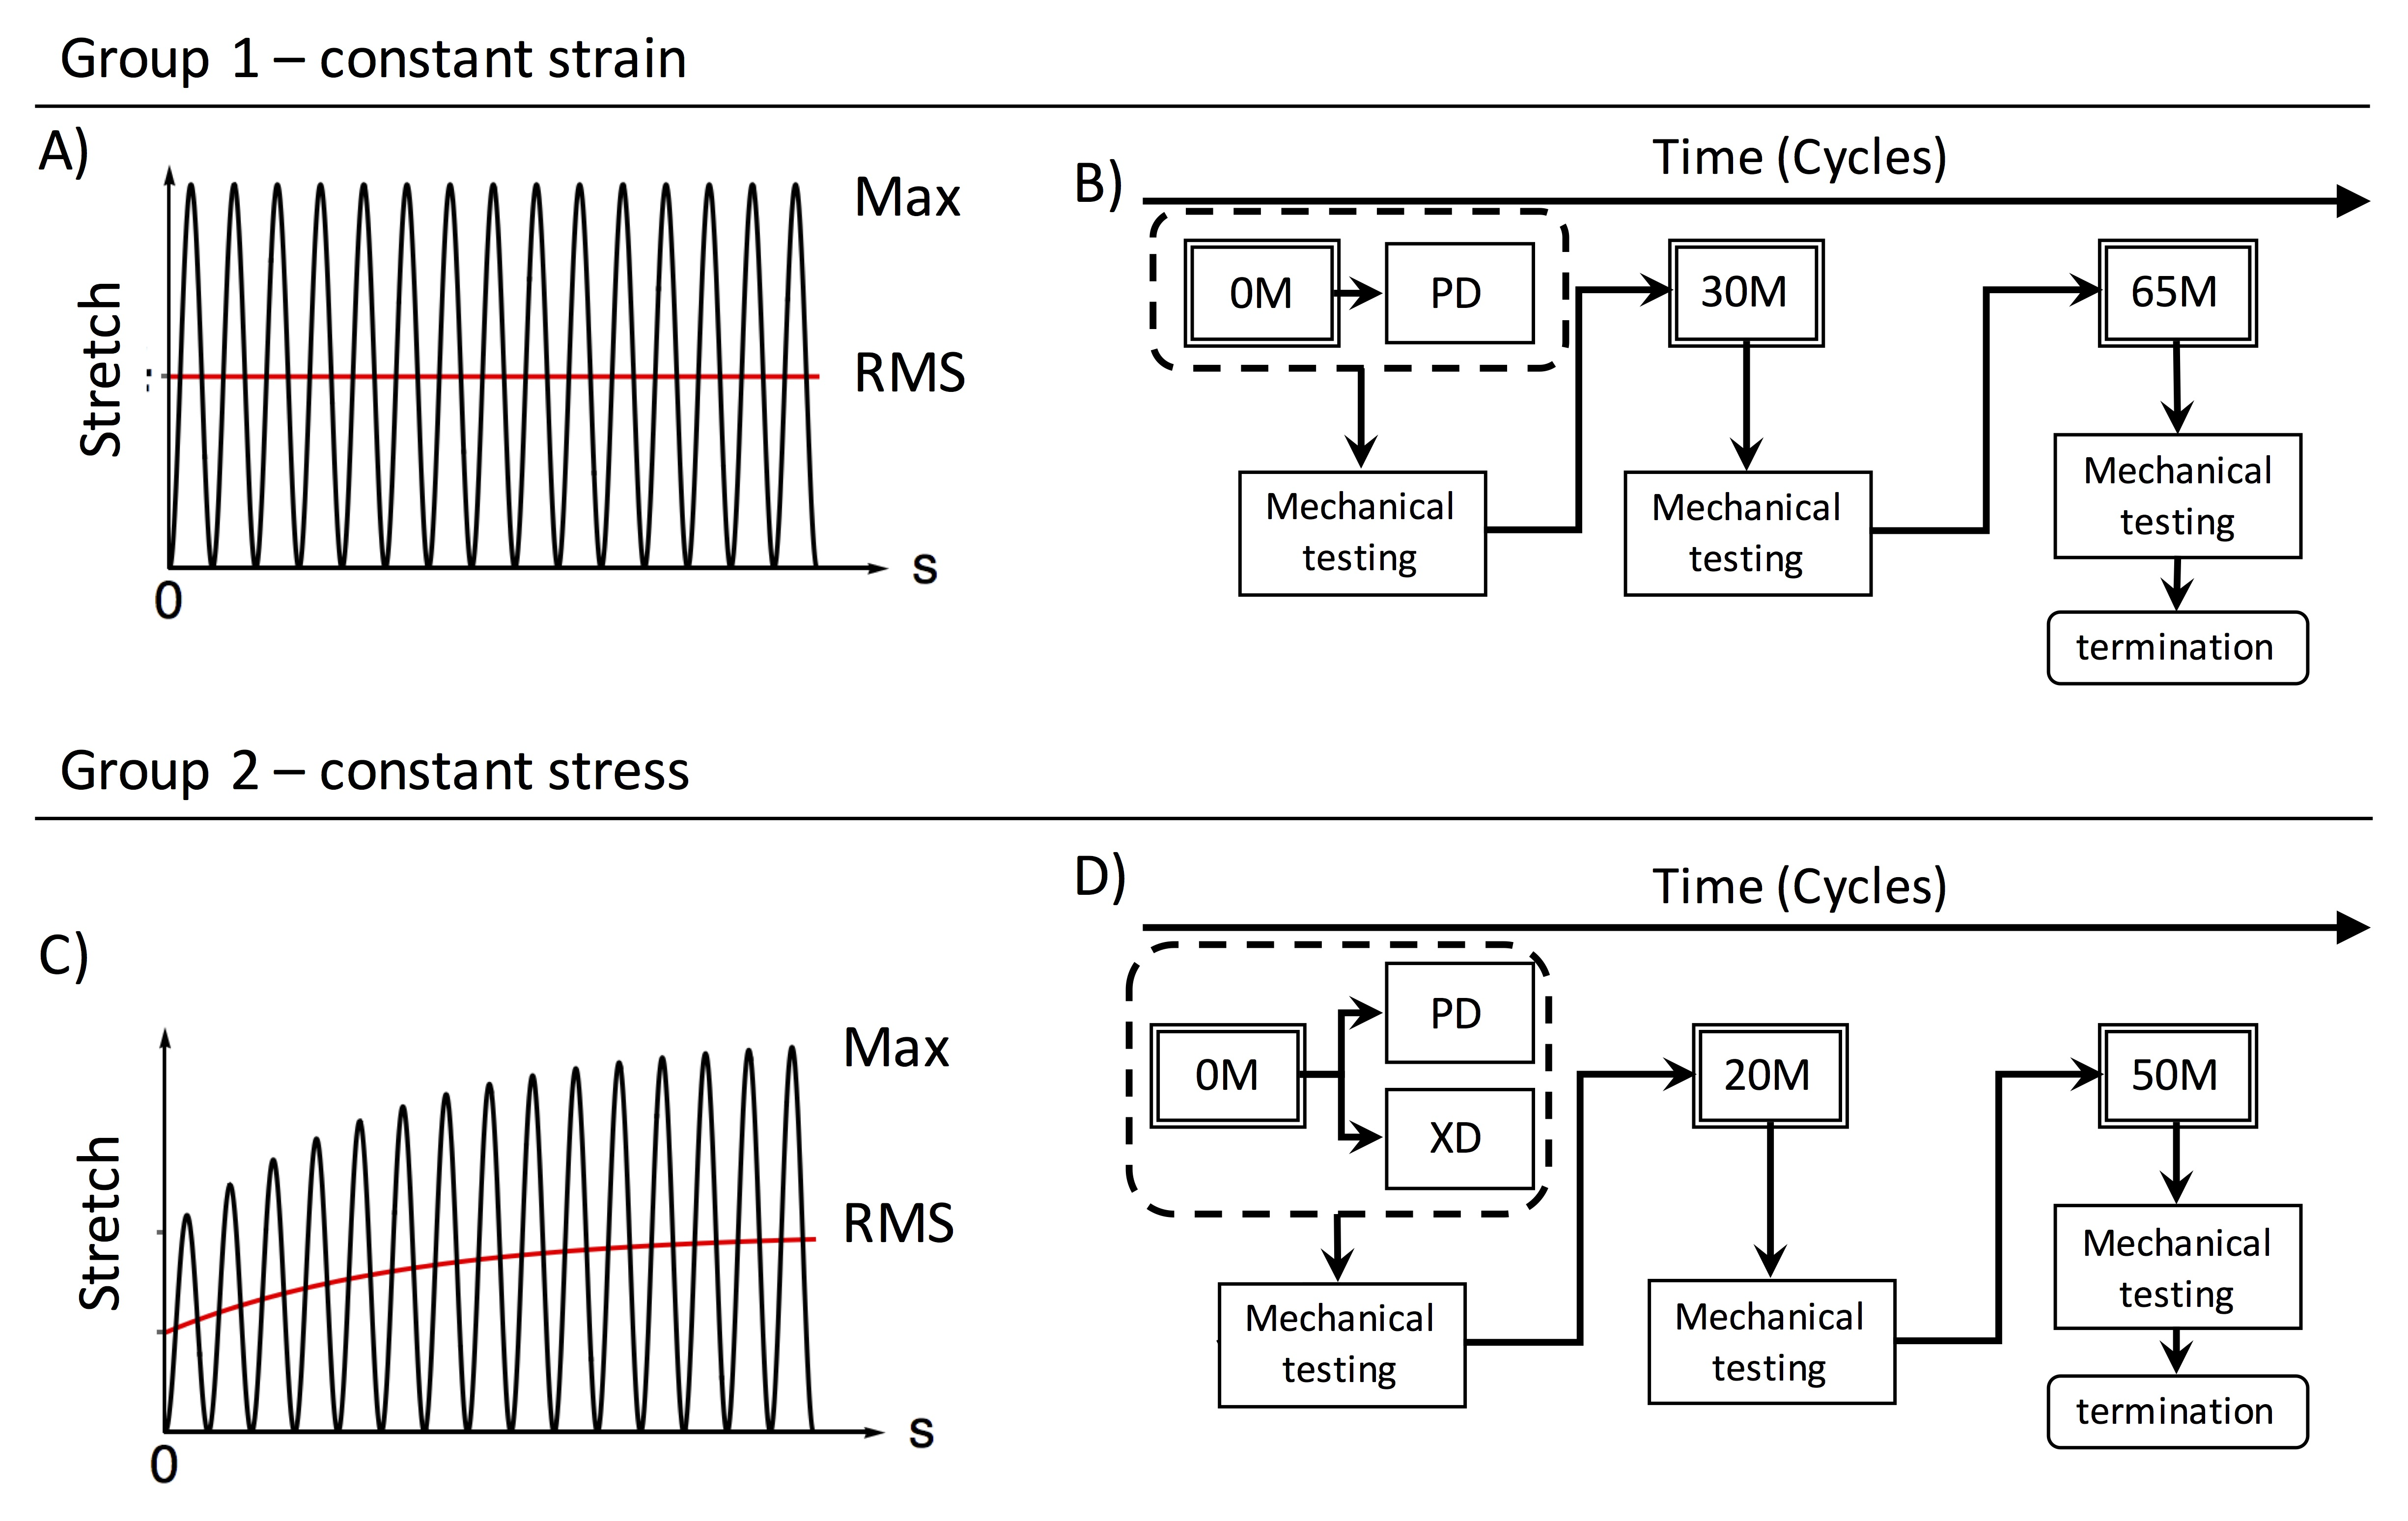
\includegraphics[width=\textwidth]{Images/chapter4/figure5}
\caption{We utilize two extant databases in this study. The first is strain controlled, with A) constant strain level and is B) sorted for orientation along the preferred direction then put through cyclic loading and mechanical testing. The second is with C) constant strain but evolving strain level. The specimens are then D) sorted for orientation along both the preferred direction and cross-preferred direction, then put through cyclic loading and mechanical testing.}
\label{fig:database}
\end{figure}



	In the study by Sellaro \textit{et al}.\cite{sellaro_effects_2007}, the same exogenously crosslinked BP patches were cycled at 500kPa for up to 50 million cycles (Fig. \ref{fig:database}C\&D). In this case, the specimens were separated into two groups: with stress controlled loading along the 1) PD and 2) orthogonal to the PD (XD). Similarly, the reference states of the exogenously crosslinked BP specimens were tracked, with cycling stopped at 20 and 50 million cycles for mechanical testing. Analysis of the results showed interesting differences between the PD and XD cycled specimens. For both the PD and XD cycled specimens, we observed significant elongation in the direction of loading and contraction in the orthogonal direction with cycling. Additionally, the effective stiffness in the direction of loading increased over time, whereas the orthogonal direction decreased over time. In addition, we also studied how the collagen fiber architecture of the tissue changed with cyclic loading. For the PD cycled specimens, it was observed that the collagen fiber orientation distribution became more aligned, and the collagen fiber crimp period increased from 24 $\mu$m to 28$\mu$m. On the other hand, for the XD cycled specimens, it was observed that the collagen fiber orientation distribution became more spread, and the collagen fiber crimp period remained unchanged. This findings on the structural changes with direction of cyclic loading are consistent with the structural convection that we hypothesizes with permanent set and lend further support to our model (Fig. \ref{fig:structuralconvection}). 

%---    Initial model formulation
%%%%%%%%%%%%%%%%%%%%%%%%%%%%%%%%%%%%%%%%%%%%%%%%%%%%%%%%%%%%%%%%%%%%%%%%%%%%%%%%
%%  Constitutive Model
%%%%%%%%%%%%%%%%%%%%%%%%%%%%%%%%%%%%%%%%%%%%%%%%%%%%%%%%%%%%%%%%%%%%%%%%%%%%%%%%


\section{Constitutive model for uncycled exogenously crosslinked tissue}

%%%%%%%%%%%%%%%%%%%%%%%%%%%%%%%%%%%%%%%%%%%%%%%%%%%%%%%%%%%%%%%%%%%%%%%%%%%%%%%%
%%%%    Constitutive Model for crosslinking

\subsection{Constitutive model for exogenous crosslinking}

	We have previously developed the first constitutive model for exogenously crosslinked collagenous tissues \cite{sacks_novel_2016} and determined the following three contributors to the mechanical response: collagen fibers, EXL matrix and fiber-fiber interactions, where the total strain energy density function is given by
\begin{equation} \label{eq:totalstrainenergy}
    \Psi = \phi_\mathrm{col} \left[ \Psi_\mathrm{col} + \Psi_\mathrm{int}\right] + \phi_m \Psi_m
\end{equation}
	In particular, we found the fiber ensemble interaction term ($\phi_\mathrm{col} \Psi_\mathrm{int}$) to be especially important in modeling exogenously crosslinked tissues, accounting for approximately 30\% of the stress in the fully loaded state (Fig. \ref{fig:EXLforms}A). To determine the model form of the interaction component, we used the remaining stress after subtracting the collagen fiber response and EXL matrix response from the mechanical response of the tissue after exogenous crosslinking (Fig. \ref{fig:EXLforms}A). In that study, we consider three possible forms of interactions: intra-fiber ensemble (Fig. \ref{fig:EXLforms}B) (an ensemble being a family of fibers sharing a common orientation), ensemble-ensemble rotations, and ensemble-ensemble relative extensions (Fig. \ref{fig:EXLforms}C\&D). We found that intra-fiber ensemble and ensemble-ensemble rotations were not consistent with the experimental data, whereas ensemble-ensemble extensional interactions were able to explain all of the remaining stress. 
	
\begin{figure}[hbt]
\centering
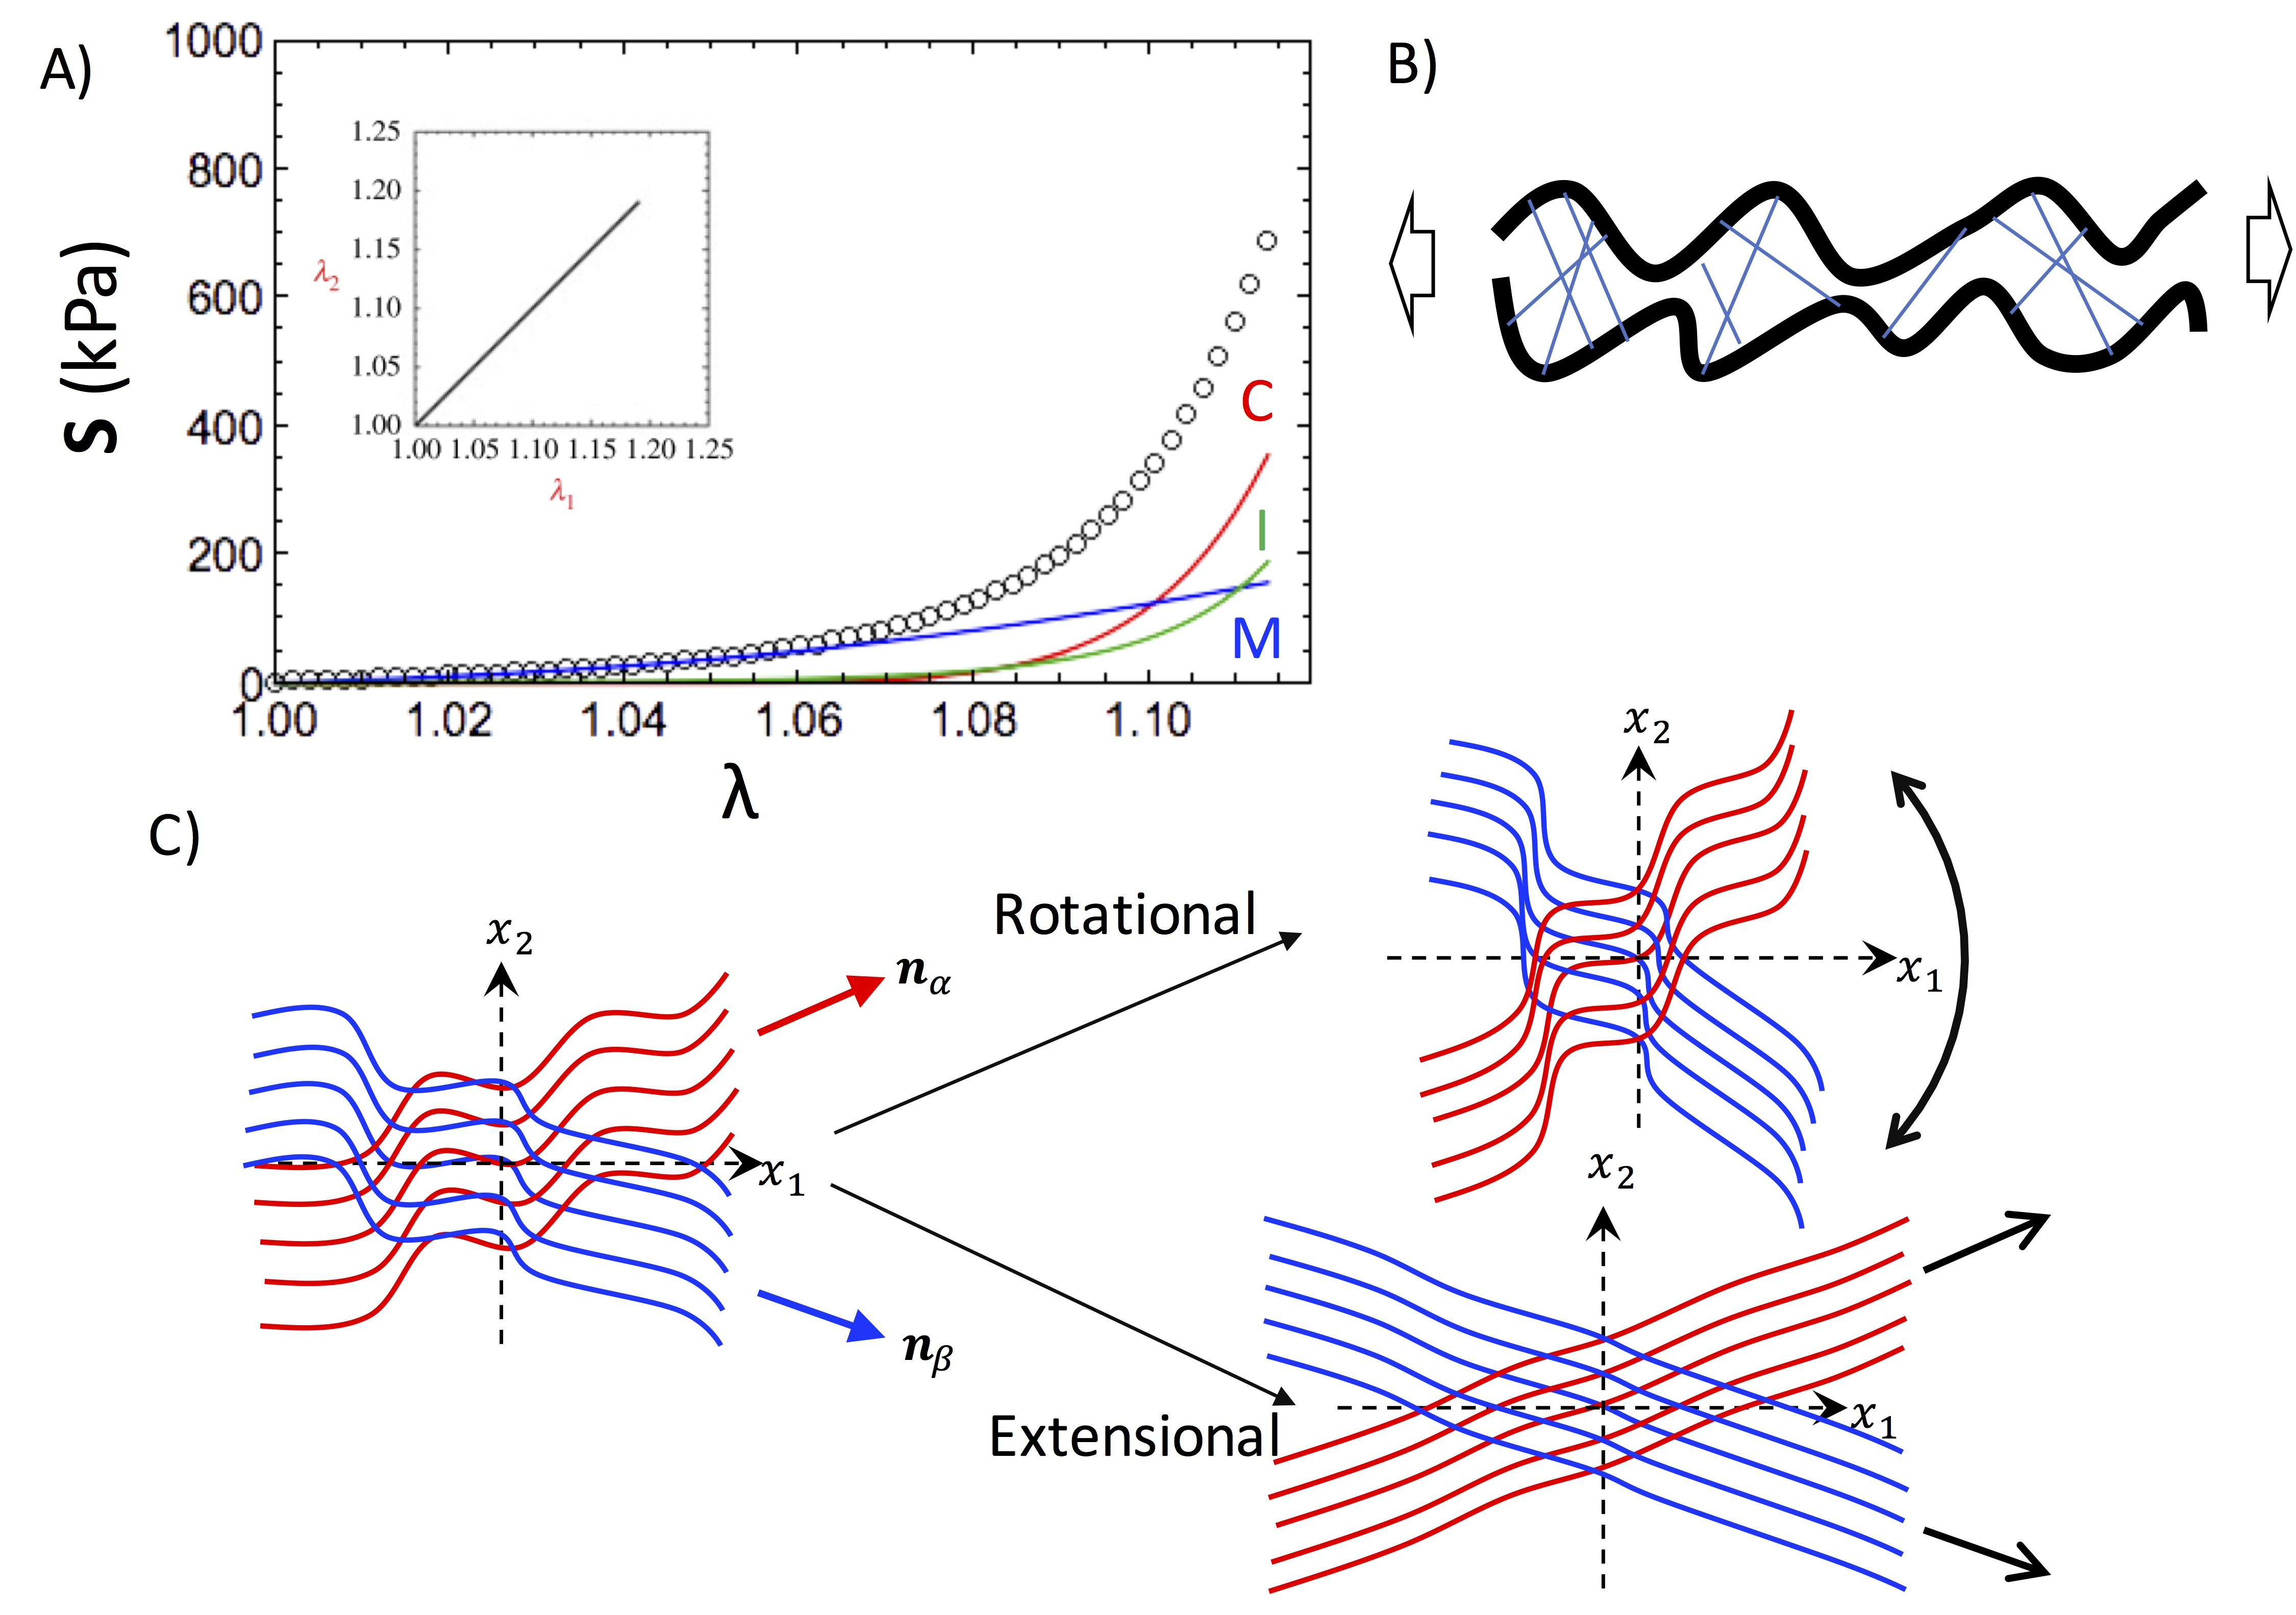
\includegraphics[width=\textwidth]{Images/chapter4/figure6}
\caption{A) The mechanical response of exogenously crosslinked BP, which is composed of 3 parts: (C)ollagen in Red, (M)atrix in Blue, and the fiber ensemble (I)nteractions in Green. B) Illustration for intra-ensemble interactions due to crosslinking is shown. C) The inter-ensemble interactions could be separated into rotational effects and extensional effects. }
\label{fig:EXLforms}
\end{figure}
	
    The interaction model form, $\Psi_\mathrm{int}$, was developed utilizing the pseudo invariant $I_8$, which is a function of the stretch and angle between two fiber ensembles oriented along the angle $\alpha$ and $\beta$ directions in the tissue (Fig. \ref{fig:structuralconvection}), and then separated it into its rotational and extensional components\cite{sacks_novel_2016} (Fig. \ref{fig:EXLforms}C\&D),
\begin{equation} \label{eq:I8invariant}
\begin{gathered}
I_8 = \mathbf{n}_ \alpha \cdot\mathbf{C}\cdot\mathbf{n}_\beta = \lambda_\alpha \lambda_\beta \cos(\alpha - \beta), \\
I_8^{\mathrm{ext}} = \lambda_\alpha \lambda_\beta, \qquad I_8^{\mathrm{rot}} = \cos(\alpha - \beta) = \frac{I_8}{\lambda_\alpha \lambda_\beta},
\end{gathered}
\end{equation}
    where $\mathbf{n}_\alpha$ and $\mathbf{n}_\beta$ are vectors pointing along $\alpha$ and $\beta$, respectively, $\lambda_\alpha$ and $\lambda_\beta$ are the stretches of the collagen fiber ensembles oriented along $\alpha$ and $\beta$, respectively , $I_8^\mathrm{ext}$ is the pseudo invariant for ensemble-ensemble extensions, and $I_8^\mathrm{rot}$ is the pseudo invariant for ensemble-ensemble rotations. From this, we established the model form for the interactions to be
\begin{equation}
\Psi_{\mathrm{int}} = \frac{d_0}{4}\int\displaylimits_\alpha \int\displaylimits_\beta \Gamma\left(\alpha\right)\Gamma \left( \beta \right)\left[ e^{d_1(\lambda_\alpha \lambda_\beta - 1)^2}-1 \right] \mathrm{d}\alpha\, \mathrm{d}\beta,
\end{equation}
    where $\Gamma$ is the fiber orientation distribution (ODF), and $d_0$ and $d_1$ are material constants. 
	However, this model form is still essentially phenomenological. 
	Specifically, while it is sufficient to model the mechanical response in the range of the acquired experimental data, we have no method for predicting how it will change with changes in dimensions with cyclic loading. Thus, an extension to this model component is necessary.

%%%%%%%%%%%%%%%%%%%%%%%%%%%%%%%%%%%%%%%%%%%%%%%%%%%%%%%%%%%%%%%%%%%%%%%%%%%%%%%%
%%%%    Extension for structural model

\subsection{Extension of the structural derivation of the fiber-fiber interactions term}

    The key to our approach in the constitutive model for the permanent set effect is to use the change in the collagen fiber architecture to predict the new mechanical response. Thus, having a full structural model, including a full structural derivation of the fiber-fiber interactions, is crucial. As in the previous model form \cite{sacks_novel_2016}, we will only keep the extensional component $I_8^\mathrm{ext}$. In addition, since collagen fibers do not bear stress until fully straightened \cite{soares_biomechanical_2016}, we also assume that \emph{collagen fibers do not play a role in the interactions of the fiber ensembles until they are straightened}. Following the same approach common in structural models, we first define the stretch of the collagen fibers after it's straightened, which is also the true fiber stretch ($\lambda_t$) defined in Zhang et al. \cite{zhang_meso_2016}, to be $\lambda_t = \lambda_\mathrm{ens}/\lambda_s$, where $\lambda_\mathrm{ens}$ is the stretch of the collagen fiber ensemble and $\lambda_s$ is the slack stretch required to straighten the collagen fiber crimp. We assumed that interactions do not occur until the fibers are straighten, so the extensional invariant should be a function of the true stretch of the individual fibers, $\lambda_t$, rather than the stretch of the whole fiber ensembles as defined in equation \ref{eq:I8invariant},
\begin{equation}
I_8^{\mathrm{ext}} = \frac{\lambda_\alpha \lambda_\beta}{\prescript{}{\alpha}{\lambda}_s \prescript{}{\alpha}{\lambda}_s},
\end{equation}
    where $\prescript{}{\alpha}{\lambda}_s$ and $\prescript{}{\beta}{\lambda}_s$ are the slack stretches of the two ensembles oriented along $\alpha$ and $\beta$ in the reference configuration, respectively. This invariant is then integrated only for fibers with $\lambda_t > 1$, i.e. fibers which are straightened. To develop the form for the interactions, we start from the strain energy. At the ensemble level, we integrate the invariant over the slack stretch $(\lambda_s)$ of both the fiber ensembles orienting along $\alpha$ and $\beta$, weighted by the probability distribution function of the proportion of collagen fibers with that specific slack stretch $D(\lambda_s)$,
\begin{equation}
\Psi_{\mathrm{int}}^{\mathrm{ens}} = \frac{\eta_I}{2} \int\displaylimits_1^{\lambda_\alpha} \int\displaylimits_1^{\lambda_\beta} D\left( x_\alpha \right) D\left( x_\beta \right) \left( \frac{\lambda_\alpha \lambda_\beta}{x_\alpha x_\beta} - 1\right)^2 \,\mathrm{d}x_\alpha \,\mathrm{d}x_\beta.
\end{equation}
    We refer to $D(\lambda_s)$ as the recruitment function, which is defined in Zhang et al. \cite{zhang_meso_2016}. The ensemble-level model is then integrated with respect to the fiber ODF, $\Gamma$, for all possible pair of collagen fiber ensemble to give the tissue-level model
\begin{equation}
\Psi_{\mathrm{int}} = \frac{\eta_I}{2} \int\displaylimits_\alpha \int\displaylimits_\beta \Gamma(\alpha) \Gamma(\beta) \int\displaylimits_1^{\lambda_\alpha} \int\displaylimits_1^{\lambda_\beta} D\left( x_\alpha \right) D\left( x_\beta \right) \left( \frac{\lambda_\alpha \lambda_\beta}{x_\alpha x_\beta} - 1\right)^2 \,\mathrm{d}x_\alpha \,\mathrm{d}x_\beta \,\mathrm{d}\alpha \,\mathrm{d}\beta.
\end{equation}
    The second Piola Kirchhoff stress, using $\mathbf{S}=2\frac{\partial\Psi}{\partial\mathbf{C}}$, is 
\begin{equation} \label{eq:interaction}
\begin{split}
\mathbf{S}_{\mathrm{int}} = \eta_I \int\displaylimits_\alpha \int\displaylimits_\beta \Gamma \left(\alpha \right) \Gamma \left( \beta \right) 
\left[ \left\lbrace 
\int\displaylimits_1^{\lambda_\alpha} \int\displaylimits_1^{\lambda_\beta} 
\frac{2 \lambda_\beta D(x_\alpha) D(x_\beta)}{x_\alpha x_\beta} 
\left( \frac{\lambda_\alpha}{x_\alpha} \frac{\lambda_\beta}{x_\beta} - 1\right) \mathrm{d}x_\alpha \, \mathrm{d}x_\beta \right.\right. +&\\
\left. \left. \int\displaylimits_1^{\lambda_\beta} D(x_\beta) \left( \frac{\lambda_\beta}{x_\beta} -1  \right)^2 \mathrm{d}x_\beta \right\rbrace \right.  \frac{\mathbf{n}_\alpha \otimes \mathbf{n}_\alpha}{\lambda_\alpha} +& \\
\left. \left\lbrace
\int\displaylimits_1^{\lambda_\alpha} \int\displaylimits_1^{\lambda_\alpha} 
\frac{2 \lambda_\beta D(x_\alpha) D(x_\beta)}{x_\alpha x_\beta} 
\left( \frac{\lambda_\alpha}{x_\alpha} \frac{\lambda_\beta}{x_\beta} - 1\right) \mathrm{d}x_\alpha \, \mathrm{d}x_\beta 
\right. \right. +&\\
\left. \left. \int\displaylimits_1^{\lambda_\alpha} D(x_\alpha) \left( \frac{\lambda_\alpha}{x_\alpha} -1  \right)^2 \mathrm{d}x_\alpha \right\rbrace \frac{\mathbf{n}_\beta \otimes \mathbf{n}_\beta}{\lambda_\beta}  \right]& \mathrm{d}\alpha \, \mathrm{d}\beta.
\end{split}
\end{equation}
    This model form has only one constant $\eta_I$ to account for all interactions. The remaining mechanisms are all based on the collagen fiber architecture, which is determined through a convection using dimensional changes. 

%---    Model simplifications and parameter estimation
%%%%%%%%%%%%%%%%%%%%%%%%%%%%%%%%%%%%%%%%%%%%%%%%%%%%%%%%%%%%%%%%%%%%%%%%%%%%%%%%
%%  Permanent Set Model
%%%%%%%%%%%%%%%%%%%%%%%%%%%%%%%%%%%%%%%%%%%%%%%%%%%%%%%%%%%%%%%%%%%%%%%%%%%%%%%%


\section{Permanent set model}

%%%%%%%%%%%%%%%%%%%%%%%%%%%%%%%%%%%%%%%%%%%%%%%%%%%%%%%%%%%%%%%%%%%%%%%%%%%%%%%%
%%%%    Kinematics

\subsection{Kinematics}

	For the bulk tissue level mechanical response, consisting of the EXL matrix, the collagen fibers, and fiber ensemble interactions, we first consider the EXL matrix alone. Permanent set occurs in the EXL matrix, and is the main driver for the evolving mechanical response and structural changes in the tissue. As such the permanent set model is our starting point (section \ref{sec:modelapproach}), which then can be used to convect collagen fiber architecture and predict the remaining collagen fibers and fiber ensemble interactions components of the mechanical response. To model the EXL matrix under permanent set, many reference states need to be considered. Due to scission-healing, the reference configuration of the EXL matrix is the configuration at its time of formation. For this we first introduce the following definition for the for the evolution of the configurations involved (Fig. \ref{fig:stateevolution}):

\begin{enumerate}

\item The original unloaded configuration $\Omega_0$ 

\item The evolving loaded configuration is $\Omega(s)$, where $s$ is the current time. 

\item We also make the distinction between $\hat{s}$, the intermediate time for which the EXL matrix is formed, and $s$. As the reference configuration of the EXL matrix evolves, there needs to be a distinction between the configuration for which the EXL matrix formed by the scission-healing reaction at time $\hat{s}$, referenced to $\Omega(\hat{s})$, and the current loaded configuration $\Omega(s)$. In this way, $\hat{s}$ is also suitable as an variable of integration.

\item The strain history, $\mathbf{A}(s)$, which is a deformation gradient tensor as a function of time $s$, that maps between the original configuration $\Omega_0$ to the loaded configuration $\Omega(s)$ at which the EXL matrix is formed

\item We define $\tilde{\mathbf{B}}(s) = \mathbf{A}\mathbf{A}^\mathsf{T}$ to be left Cauchy Green tensor of the strain history $\mathbf{A}(s)$, which should not be confused with the left Cauchy Green tensor of the deformation applied to the tissue

\item We define the deformation gradient tensor from the intermediate loaded state $\Omega(\hat{s})$ to the current loaded state $\Omega(s)$ to be $\mathbf{\bar{F}}(\hat{s})$, where the following relation is assumed (Fig. \ref{fig:stateevolution})
\begin{equation} \label{eq:strainhistory}
\begin{split}
&\mathbf{F} = \mathbf{\bar{F}}(\hat{s})\mathbf{A}(\hat{s}), \\
&\mathbf{\bar{F}}(\hat{s}) = \mathbf{F} \cdot \mathbf{A}(\hat{s})^{-1}.
\end{split}
\end{equation}

\item The evolving unloaded reference configuration after permanent set is $\Omega_\mathrm{PS}(s)$ with $\mathbf{F}_\mathrm{PS}(s)$ mapping from the original configuration $\Omega_0$ to $\Omega_\mathrm{PS}(s)$

\end{enumerate}

\begin{figure}[hbt]
\centering
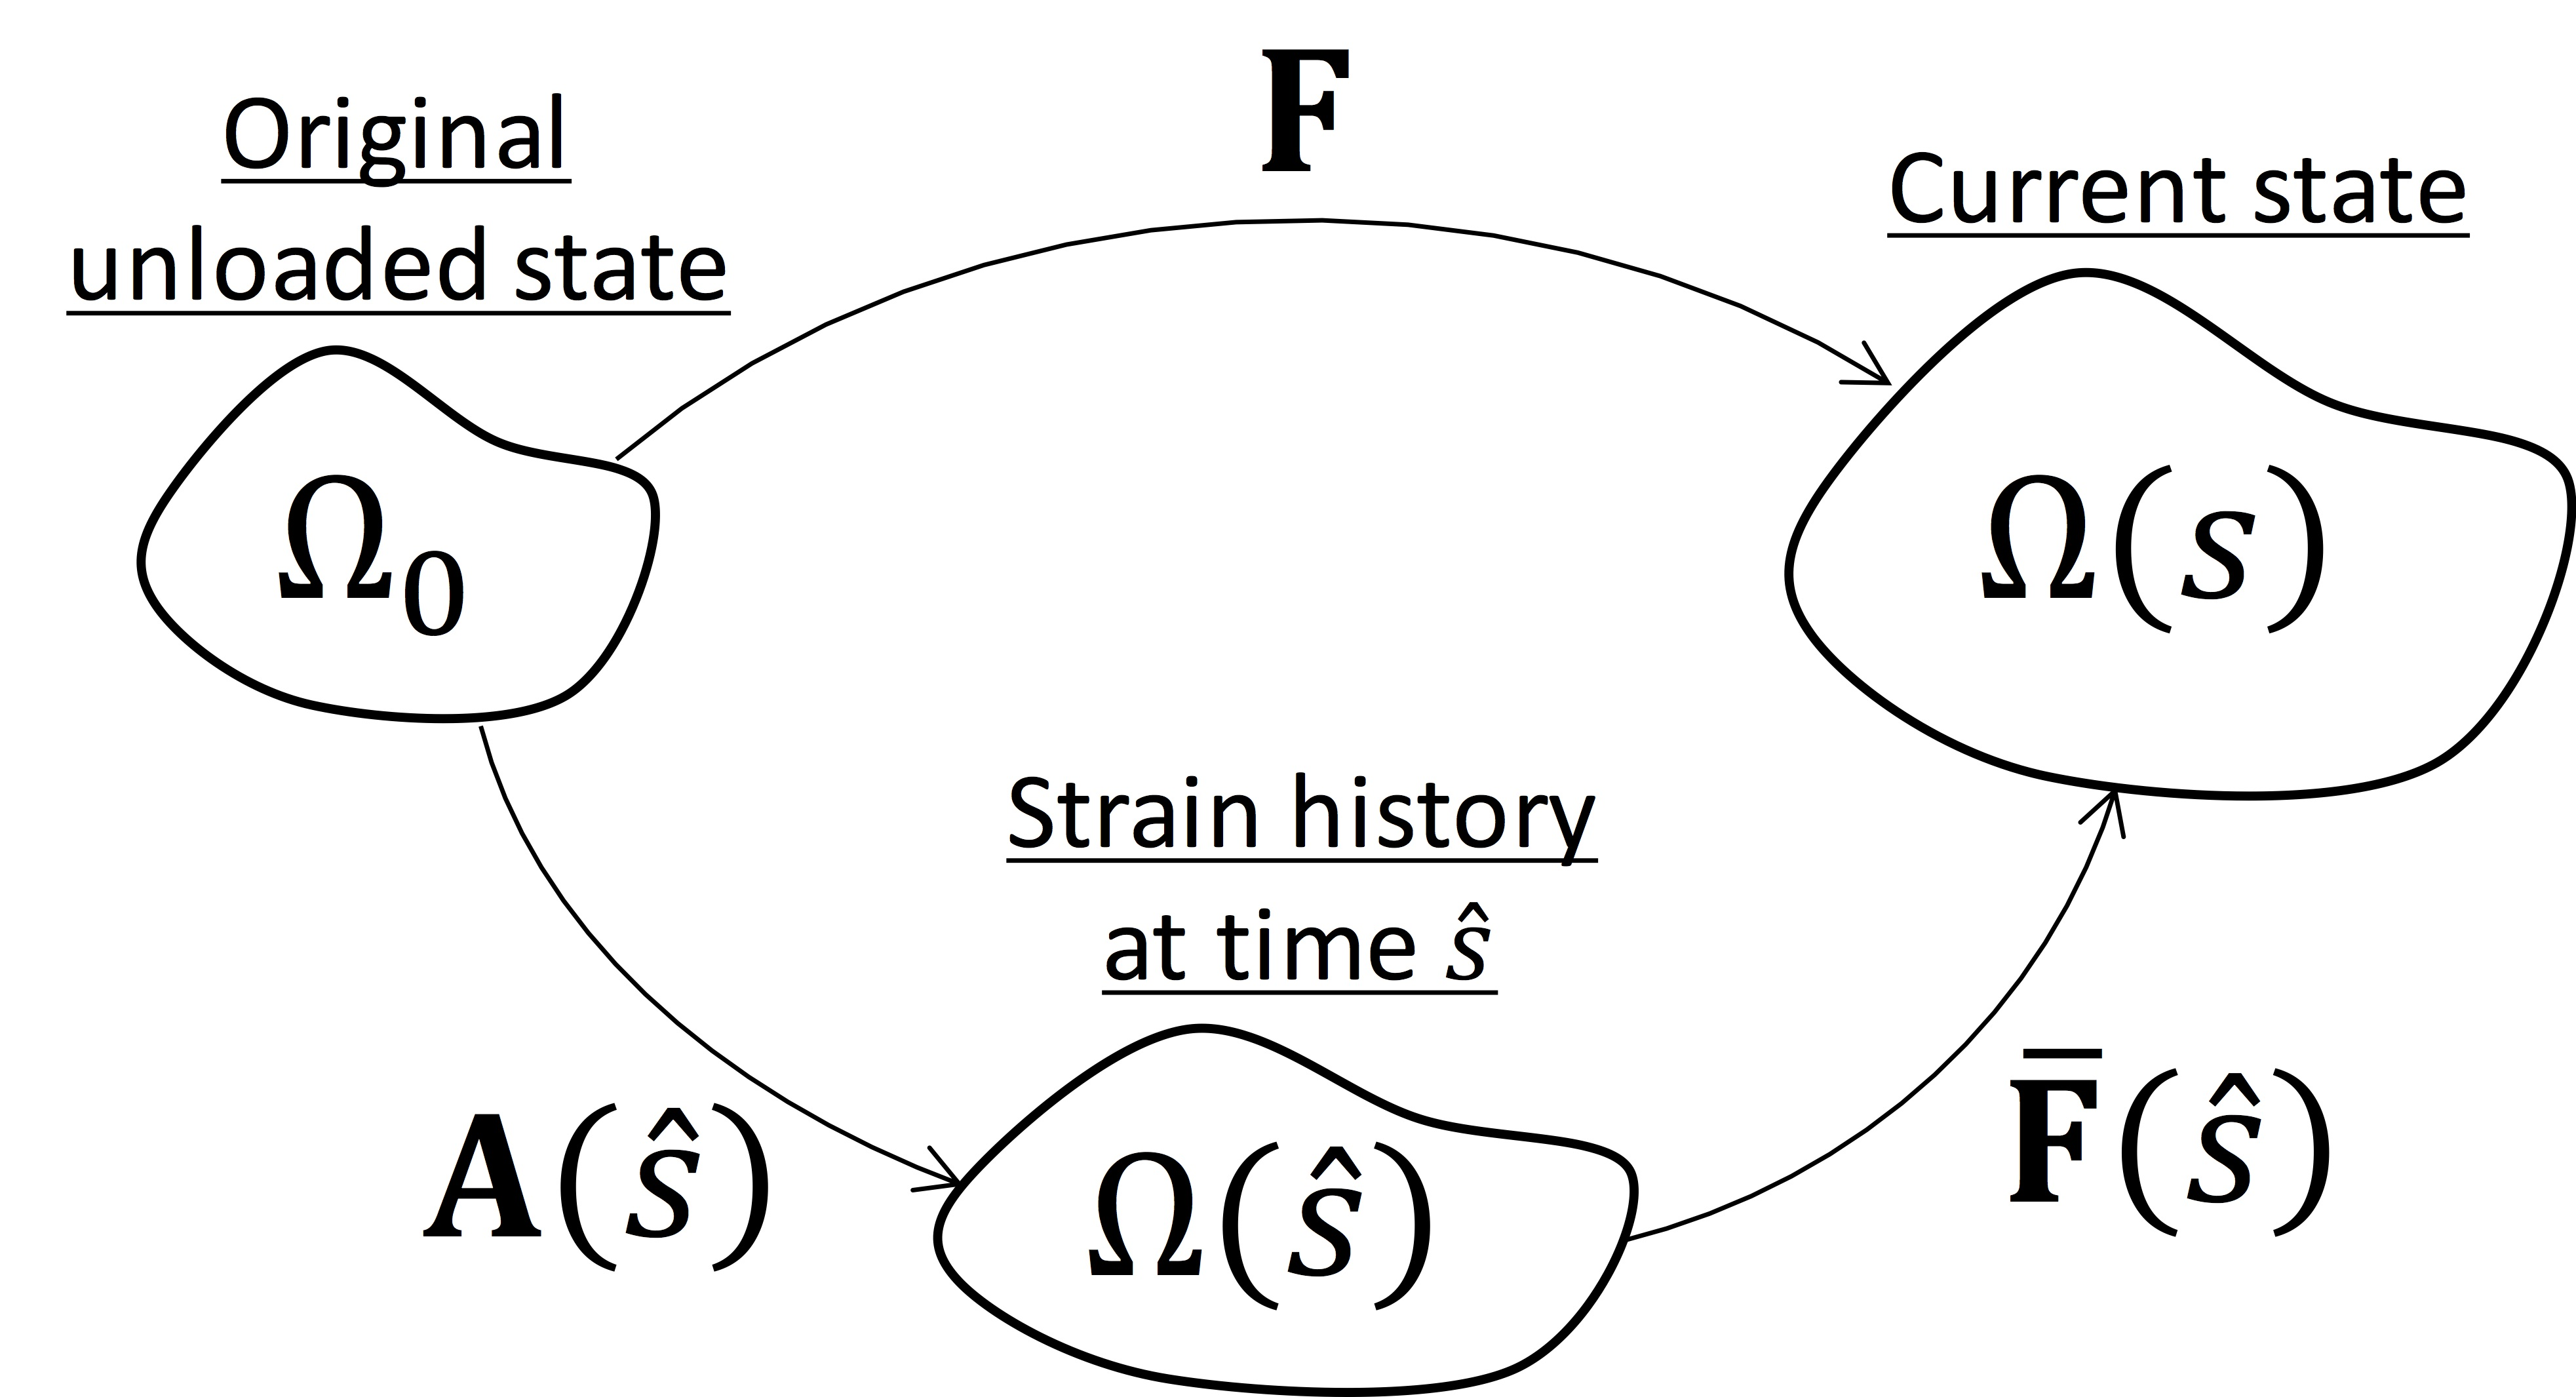
\includegraphics[width=3.5in]{Images/chapter4/figure7}
\caption{The relation between the reference configurations during cyclic loading.}
\label{fig:stateevolution}
\end{figure}

    We also note the following important considerations:
\begin{itemize}
\item The original reference configuration $\Omega_0$ is important as it is the configuration for which the mechanical response of the original material as well as the collagen fiber architecture is referenced. Similarly, we track the loaded configuration ($\Omega(s)$) using $\mathbf{A}(s)$ and the unloaded configuration ($\Omega_\mathrm{PS}(s)$) using $\mathbf{F}_\mathrm{PS}$ from $\Omega_0$. 

\item We also note that under cyclic loading, the exogenously crosslinked tissue is not held at the constant loaded configuration, it is put through a range of deformation each cycle. Because permanent set happens at a time scale much longer than a single cycle, we define the loaded configuration $\Omega(s)$ as the root mean squared configuration, which is the time averaged deformation for a single loading cycle. 

\item We note that the tissue is never fully unloaded during cyclic loading. Thus, to simulate cyclic loading, the stresses are still referenced to the origin configuration $\Omega_0$. The unloaded geometry is determined \textit{a posteriori} from $\Omega_\mathrm{PS}(s)$ for when cyclic loading is stopped for mechanical testing. 
\end{itemize}



    Thus the right Cauchy Green tensor when referenced to the strain history $\Omega(\hat{s})$ is given by $\mathbf{\bar{C}}(\hat{s}) = \mathbf{\bar{F}}(\hat{s})^\mathsf{T} \mathbf{\bar{F}}(\hat{s})$. This also has the following relation to the applied deformation $\mathbf{F}$,
\begin{equation} \label{eq:rightcauchy}
\begin{split}
\mathbf{\bar{C}}(\hat{s}) &= \left( \mathbf{F}\cdot\mathbf{A}(\hat{s})^{-1} \right)^\mathsf{T} \left(\mathbf{F} \cdot \mathbf{A}(\hat{s})^{-1} \right)\\
	&= \mathbf{A}(\hat{s})^{-\mathsf{T}} \left( \mathbf{F}^\mathsf{T} \mathbf{F} \right) \mathbf{A}(\hat{s})^{-1} \\
	&= \mathbf{A}(\hat{s})^{-\mathsf{T}} \cdot \mathbf{C} \cdot \mathbf{A}(\hat{s})^{-1}.
\end{split}
\end{equation}
    Our material model for the EXL matrix is an isotropic model of $\Psi_m = \Psi_m(I_1)$, where $I_1$ is the first invariant of $\mathbf{C}$. For this, we can define the first invariant $\bar{I}_1(\hat{s})$ for the right Cauchy Green tensor $\bar{\mathbf{C}}(\hat{s})$ as 
\begin{equation}\label{eq:pseudo1stinv}
\bar{I}_1(\hat{s}) = \operatorname{Trace}(\mathbf{\bar{C}}(\hat{s})) = \operatorname{Trace}\left(\mathbf{A}^{-\mathsf{T}}(\hat{s}) \cdot \mathbf{C} \cdot \mathbf{A}^{-1}(\hat{s})\right).
\end{equation}
    With this, the stress of the EXL matrix is given by 

\begin{equation}
\mathbf{\bar{S}}_m = 2 \frac{\partial \bar{\Psi}}{\partial \mathbf{C}} - p\mathbf{I} = 2 \frac{\partial \bar{\Psi}}{\partial \bar{I}_1(\hat{s})} \frac{\partial \bar{I}_1(\hat{s})}{\partial \mathbf{C}} - p\mathbf{I},
\end{equation}
    where $p$ is the Lagrange multiplier enforcing incompressibility. The partial derivative of $\bar{I}_1(\hat{s})$ is
\begin{equation}
\frac{\partial\bar{I}_1}{\partial\mathbf{C}} = \frac{\partial\bar{I}_1}{\partial\bar{\mathbf{C}}(\hat{s})} \frac{\partial\bar{\mathbf{C}}(\hat{s})}{\partial \mathbf{C}}= \frac{\partial\mathbf{A}(\hat{s})^{-\mathsf{T}} \cdot \mathbf{C} \cdot \mathbf{A}(\hat{s})^{-1}}{\partial \mathbf{C}} = \mathbf{A}(\hat{s})^{-\mathsf{T}} \mathbf{A}(\hat{s})^{-1} = \mathbf{\tilde{B}}(\mathbf{A}(\hat{s}))^{-1},
\end{equation}
    which is the inverse of the left Cauchy Green tensor of the strain history $\mathbf{A(s)}$.


%%%%%%%%%%%%%%%%%%%%%%%%%%%%%%%%%%%%%%%%%%%%%%%%%%%%%%%%%%%%
%%%%%%      Constitutive Model for crosslinking

\subsubsection{Kinematics for updating the reference configuration}

    As the unloaded configuration changes due to permanent set, we need to be able to express the stresses with the new reference configuration. Since all configurations are referenced to $\Omega_0$, the deformation from the new reference configuration $\Omega_\mathrm{PS}$ to the current loaded state $\Omega(s)$ is given by (Fig. \ref{fig:PSevolution})
\begin{equation}
\mathbf{F} = \mathbf{\bar{F}}(\hat{s}) \cdot \mathbf{A}(\hat{s}) \cdot \mathbf{F}_\mathrm{PS}^{-1}.
\end{equation}
    Following the same derivation as equations \ref{eq:strainhistory}--\ref{eq:pseudo1stinv}, we have
\begin{equation} \label{eq:newhistory}
\begin{split}
\mathbf{\bar{F}}(\hat{s}) &= \mathbf{F} \cdot \mathbf{F}_\mathrm{PS} \cdot \mathbf{A}(\hat{s})^{-1},\\
\mathbf{\bar{C}}(\mathbf{F}_\mathrm{PS}, \mathbf{A}(\hat{s})) &= \mathbf{A}(\hat{s})^{-\mathsf{T}} \cdot \mathbf{F}_\mathrm{PS}^\mathsf{T} \cdot \mathbf{C} \cdot \mathbf{F}_\mathrm{PS} \cdot \mathbf{A}(\hat{s})^{-1}, \\
\bar{I}_1\left(\mathbf{F}_\mathrm{PS}, \mathbf{A}(s)\right) &= \operatorname{Trace}\left(\mathbf{A}(\hat{s})^{-\mathsf{T}} \cdot \mathbf{F}_\mathrm{PS}^\mathsf{T} \cdot \mathbf{C} \cdot \mathbf{F}_\mathrm{PS} \cdot \mathbf{A}(\hat{s})^{-1}\right). 
\end{split}
\end{equation}
    and the new inverse of the left Cauchy Green tensor of the strain history is given by
\begin{equation}
\begin{split}
\mathbf{\tilde{B}}(\mathbf{F}_\mathrm{PS}, \mathbf{A}(\hat{s}))^{-1} &= \frac{\partial \mathbf{\bar{C}}(\mathbf{F}_\mathrm{PS}, \mathbf{A}(\hat{s}))}{\partial \mathbf{C}} = \frac{\mathbf{A}(\hat{s})^{-\mathsf{T}} \cdot \mathbf{F}_\mathrm{PS}^\mathsf{T} \cdot \mathbf{C} \cdot \mathbf{F}_\mathrm{PS} \cdot \mathbf{A}(\hat{s})^{-1}}{\partial \mathbf{C}} \\
 &= \mathbf{A}(\hat{s})^{-\mathsf{T}} \cdot \mathbf{F}_\mathrm{PS}^\mathsf{T} \cdot \mathbf{F}_\mathrm{PS} \cdot \mathbf{A}(\hat{s})^{-1}. 
\end{split}
\end{equation}

\begin{figure}[hbt]
\centering
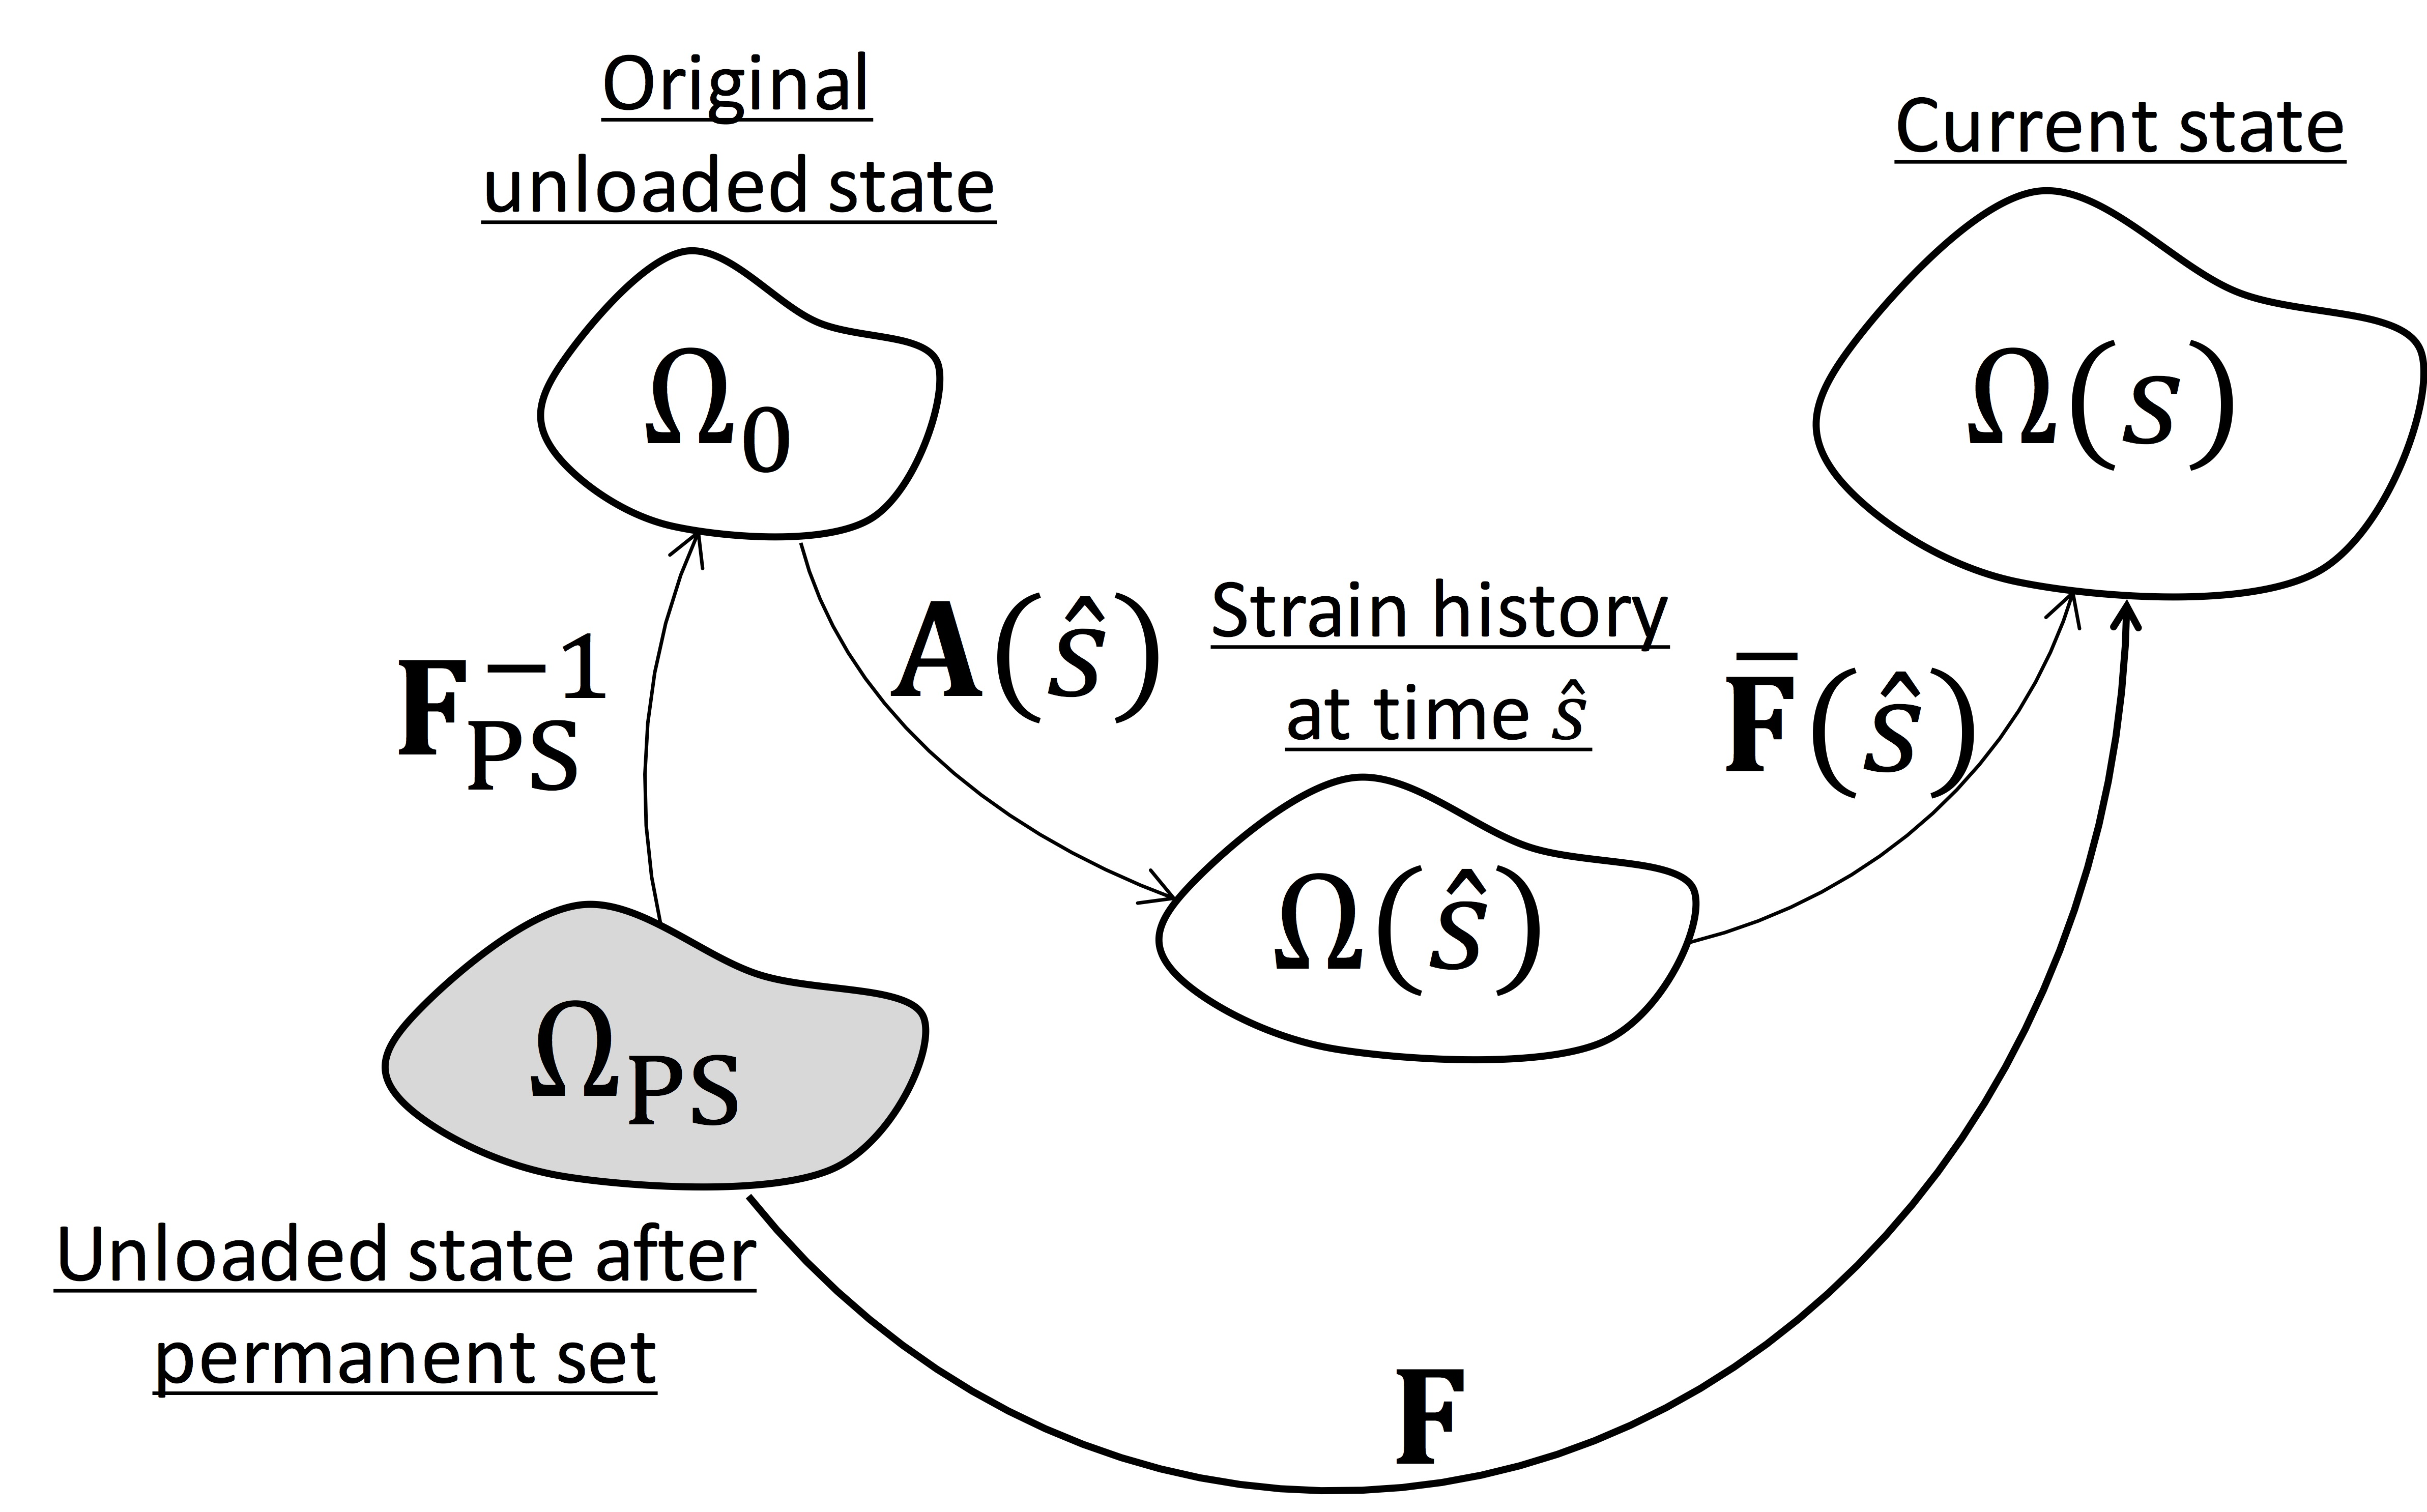
\includegraphics[width=4in]{Images/chapter4/figure8}
\caption{Modification of the relation between the different reference configurations when the unloaded configuration changes.}
\label{fig:PSevolution}
\end{figure}


%%%%%%%%%%%%%%%%%%%%%%%%%%%%%%%%%%%%%%%%%%%%%%%%%%%%%%%%%%%%%%%%%%%%%%%%%%%%%%%%
%%%%    Change in reference configuration

\subsection{Extension to the EXL matrix model for changes in reference configuration}

	We start by extending the EXL matrix model from our previous model \cite{sacks_novel_2016}. The strain energy is a modified form of the Yeoh model, which exhibits the following stress-strain relation,
\begin{equation}
\begin{split}
\Psi_m = &\frac{\eta_m}{2} \left( \frac{1}{\alpha}\left( I_1 -3\right)^{\alpha} + \frac{r}{\beta} \left( I_1 -3\right)^{\beta} \right), \\
&\text{with } 1<\alpha<\beta, \alpha\beta <2, 0 \leq r.
\end{split}
\end{equation}
    Here $\eta_m$ is the EXL matrix modulus, $\alpha,\beta$ are the exponent and $r$ is the relative weight between the two terms which is typically between 10 to 20. To modify the model form to reference the configuration at the time of formation $\Omega(\hat{s})$, we make the substitution for $\bar{I}_1(\mathbf{F}_\mathrm{PS}, \mathbf{A}(\hat{s}))$ (Eqn. \ref{eq:pseudo1stinv}),
\begin{equation} \label{eq:matrixenergyform}
\bar{\Psi}_m\left( \mathbf{C}, \mathbf{A}(\hat{s})\right) = \frac{\eta_m}{2} \left(\frac{1}{\alpha} \left( \bar{I}_1\left(\mathbf{F}_\mathrm{PS}, \mathbf{A}(s)\right) -3\right)^\alpha +\frac{r}{\beta} \left( \bar{I}_1\left(\mathbf{F}_\mathrm{PS}, \mathbf{A}(s)\right) -3\right)^\beta \right),
\end{equation}
    The derivative of the strain energy with respect to the invariant $\bar{I}_1$ is 
\begin{equation}
\frac{\partial \bar{\Psi}}{\partial \bar{I}_1} =	\frac{\eta_m}{2} \left(\left( \bar{I}_1\left(\mathbf{F}_\mathrm{PS}, \mathbf{A}(s)\right)- 3\right)^{\alpha - 1} + r \left( \bar{I}_1\left(\mathbf{F}_\mathrm{PS}, \mathbf{A}(s)\right) - 3\right)^{\beta - 1}\right).
\end{equation}
    After solving for the Lagrange multiplier $p$, with $\bar{S}_{m,33} = 0$, we have 
\begin{equation}\label{eq:matrixfinal}
\begin{split}
\mathbf{\bar{S}}_m \left( \mathbf{F}_\mathrm{PS},\mathbf{A}(\hat{s}),\mathbf{C}\right) &= \mu_m \left(\left( \bar{I}_1\left(\mathbf{F}_\mathrm{PS}, \mathbf{A}(s)\right) - 3\right)^{\alpha - 1} + r \left( \bar{I}_1\left(\mathbf{F}_\mathrm{PS}, \mathbf{A}(s)\right) - 3\right)^{\beta - 1}\right) \\
&\times \left( \mathbf{\tilde{B}}(\mathbf{F}_\mathrm{PS}, \mathbf{A}(\hat{s}))^{-1} - \tilde{B}_{33}^{-1}(\mathbf{F}_\mathrm{PS}, \mathbf{A}(\hat{s}))C_{33}\mathbf{C}^{-1}\right).
\end{split}
\end{equation}


%%%%%%%%%%%%%%%%%%%%%%%%%%%%%%%%%%%%%%%%%%%%%%%%%%%%%%%%%%%%
%%%%%%      Extension for permanent set

\subsubsection{Extension of the EXL matrix for the permanent set effect}

	Next, we developed the model form for the EXL matrix after permanent set. This approach is based on the work by Rajagopal and Wineman \cite{rajagopal_constitutive_1992}, where we assume that the response of the full EXL matrix to be 
\begin{equation} \label{eq:wineman}
\phi_m \mathbf{S}_m = b(s)\mathbf{\bar{S}}_m^\mathrm{existing} + \int\displaylimits_0^s a(s,\hat{s})\mathbf{\bar{S}}_m^\mathrm{new} \mathrm{d}\hat{s},
\end{equation}
    where $b(s)$ is the remaining amount of the existing material, $a(s,\hat{s})$ is the remaining amount of the new material formed during the strain history ($\mathbf{A}(s)$) at time $\hat{s}$, $\mathbf{\bar{S}}_m^\mathrm{existing}$ is the stress of the existing material and $\mathbf{\bar{S}}_m^\mathrm{new}$ is the stress of the new material. Assuming first order kinetics with the permanent set rate constant $k $, we have for the material remaining (Fig. \ref{fig:masstransfer})
\begin{equation}
\frac{\partial b(s)}{\partial s} = - k\cdot b(s), \qquad \frac{\partial a(s,\hat{s})}{\partial s} = - k \cdot a(s,\hat{s}).
\end{equation}
    Given that the total amount of EXL matrix ($\phi_m$) has not changed, $b(s) + \int_0^s a(s, \hat{s}) \mathrm{d}\hat{s} = \phi_m$, and we have
\begin{equation}
b(s) = \phi_m \mathrm{Exp}\left[-k  \cdot s\right], \qquad a(s,\hat{s}) = \phi_m k  \mathrm{Exp}\left[-k (s - \hat{s})\right].
\end{equation}
    Substitution into equation \ref{eq:wineman}, we have the mechanical response of the EXL matrix after permanent set,
\begin{equation}
\phi_m \mathbf{S}_m = \phi_m \left[\mathrm{Exp}\left[-k  \cdot s\right]\mathbf{\bar{S}}_m \left(\mathbf{F}_\mathrm{PS},\mathbf{A}(0),\mathbf{C}\right) + \int\displaylimits_0^s k \cdot \mathrm{Exp}\left[-k (s - \hat{s})\right] \mathbf{\bar{S}}_m \left(\mathbf{F}_\mathrm{PS},  \mathbf{A}(\hat{s}),\mathbf{C}\right) \mathrm{d}\hat{s} \right].
\end{equation}
    The final form for the EXL matrix component of the permanent set model is thus,
\begin{equation}
\begin{split}
\phi_m \mathbf{S}_m \left(\mathbf{F}_\mathrm{PS}, \mathbf{A}(\hat{s}),\mathbf{C}\right) &= \phi_m \mu_m \left[ \vphantom{\int\displaylimits_0^s} \mathrm{Exp}\left[-k  \cdot s\right]  \left(\left( \bar{I_1} (\mathbf{F}_\mathrm{PS}, \mathbf{A}(0)) - 3\right)^{\alpha - 1} + r \left( \bar{I_1} (\mathbf{F}_\mathrm{PS}, \mathbf{A}(0)) - 3\right)^{\beta - 1}\right)  \right.\\
&\times \left( \mathbf{\tilde{B}}(\mathbf{F}_\mathrm{PS}, \mathbf{A}(0))^{-1} - \tilde{B}_{33}(\mathbf{F}_\mathrm{PS}, \mathbf{A}(0))^{-1}C_{33}\mathbf{C}^{-1}\right) \\
&+ \int\displaylimits_0^s k \cdot \mathrm{Exp}\left[-k (s - \hat{s})\right] \left(\left( \bar{I_1} (\mathbf{F}_\mathrm{PS}, \mathbf{A}(\hat{s})) - 3\right)^{\alpha - 1} + r \left( \bar{I_1} (\mathbf{F}_\mathrm{PS}, \mathbf{A}(\hat{s})) - 3\right)^{\beta - 1}\right) \\
&\times \left. \vphantom{\int\displaylimits_-^s} \left( \mathbf{\tilde{B}}(\mathbf{F}_\mathrm{PS}, \mathbf{A}(\hat{s}))^{-1} - \tilde{B}_{33}(\mathbf{F}_\mathrm{PS}, \mathbf{A}(\hat{s}))^{-1}C_{33}\mathbf{C}^{-1}\right) \mathrm{d}\hat{s}\right].
\end{split}
\end{equation}

\begin{figure}[hbt]
\centering
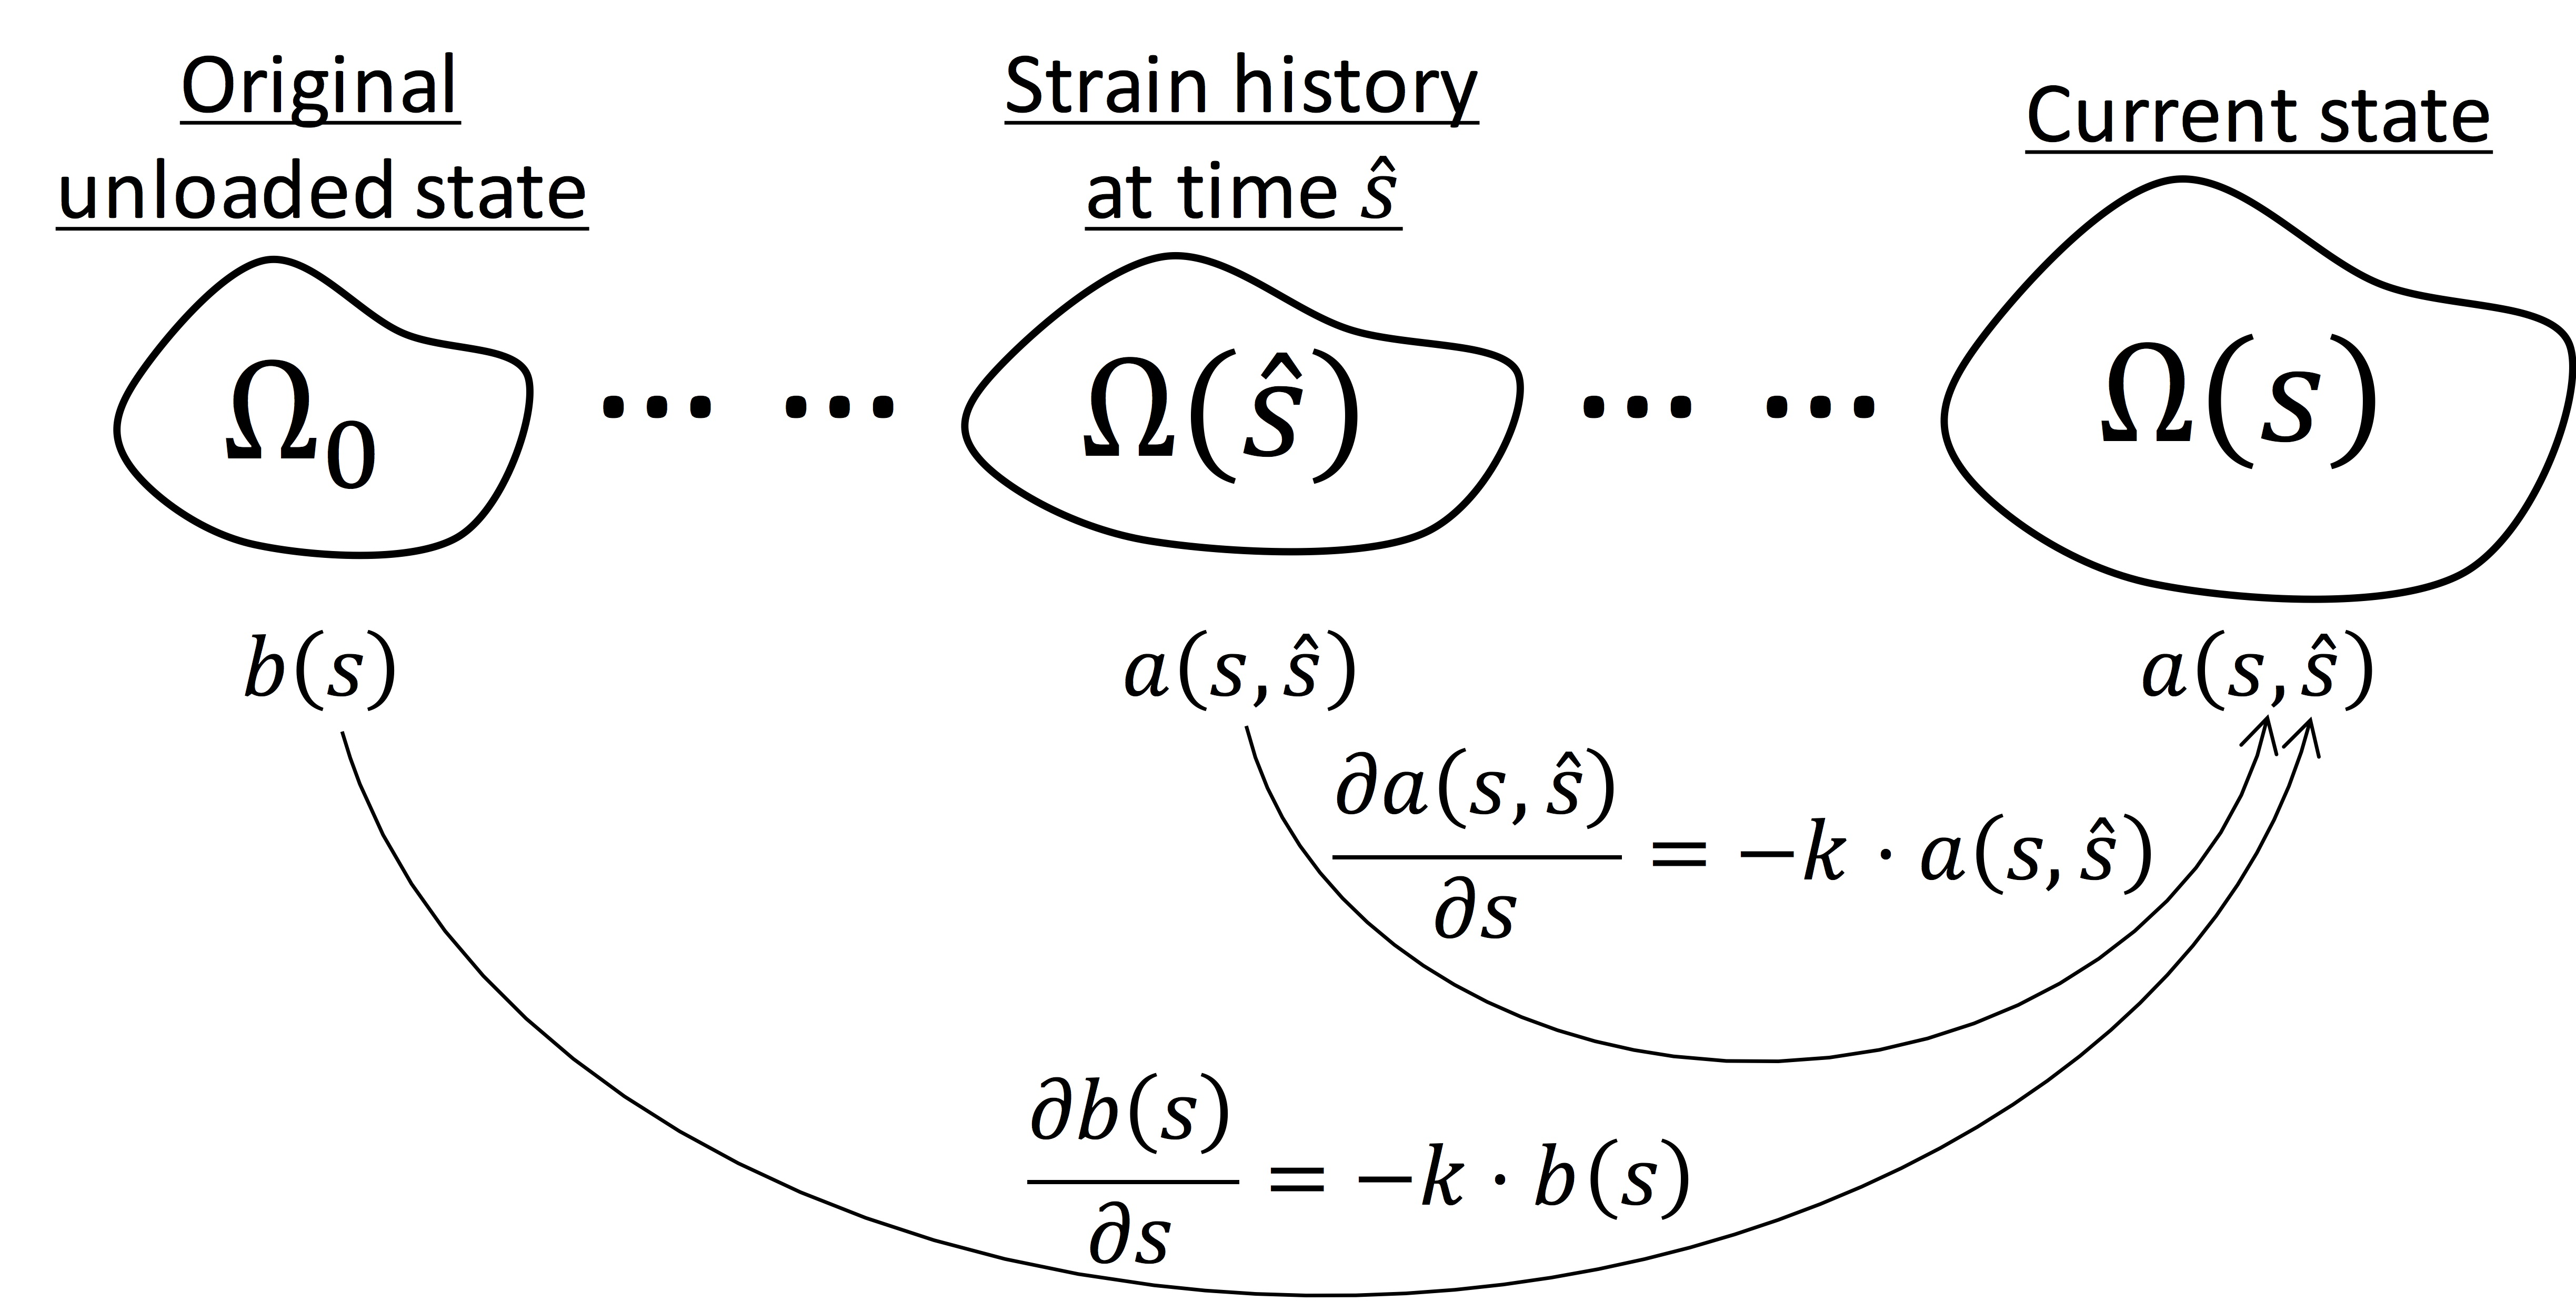
\includegraphics[width=4.5in]{Images/chapter4/figure9}
\caption{The mass fractions of the EXL matrix change over time, assuming first order kinetics. }
\label{fig:masstransfer}
\end{figure}

%%%%%%%%%%%%%%%%%%%%%%%%%%%%%%%%%%%%%%%%%%%%%%%%%%%%%%%%%%%%%%%%%%%%%%%%%%%%%%%%
%%%%    Structural Convection

\subsection{Convection of the collagen fiber architecture} \label{sec:convection}

    Now that the model form for the EXL matrix under permanent set is established, we need to consider how the collagen fiber architecture is convected by the change in reference configuration. The convection of the collagen fiber architecture is done through two parts: the ODF and the recruitment function. This is done by assuming that the collagen fiber architecture is convected under the affine assumption\cite{lee_presence_2015}. The form of the ODF and the recruitment distribution was previously described in Zhang \textit{et al.} \cite{zhang_meso_2016}, and the operation used to convect the collagen fiber architecture is given in Sacks \textit{et al}. \cite{sacks_novel_2016}. Briefly, the convected ODF $\Gamma_1$ is determined from the ODF in the 0-cycle state $\Gamma_0$ and the deformation $\prescript{1}{0}{\mathbf{F}}$ by the conservation of the number of fiber $\Gamma(\theta_0) \mathrm{d}\theta_0 = \Gamma(\theta_1) \mathrm{d}\theta_1$ (Fig. \ref{fig:effectsofconvection}A). This is given by
\begin{equation} \label{eq:pfODF}
\begin{gathered}
\Gamma_1\left( \prescript{1}{0}{\mathbf{F}},\theta_1 \right) = \Gamma_0\left( \theta_0\left( \prescript{1}{0}{\mathbf{F}},\theta_1\right)\right)\frac{\prescript{1}{0}{\lambda(\theta_0)}^2}{\prescript{1}{0}{J_\mathrm{2D}}}, \\
\prescript{1}{0}{\lambda(\theta_0)} = \sqrt{\mathbf{n}_{\theta_0}\cdot  \prescript{1}{0}{\mathbf{F}^\mathsf{T}}  \prescript{1}{0}{\mathbf{F}} \cdot \mathbf{n}_{\theta_0}}, \qquad \prescript{1}{0}{J_\mathrm{2D}} =\det (\prescript{1}{0}{\mathbf{F}}),
\end{gathered}
\end{equation}
    where $\mathbf{n}_\theta$ is a unit vector for the orientation $\theta$. The distribution of slack stretch needed to straighten collagen fiber crimp after convection, in other words the recruitment distribution $D_1(\lambda_s)$ (Fig. \ref{fig:effectsofconvection}B), is given by
\begin{equation} \label{eq:pfrecruitment}
\begin{gathered}
D_1(\prescript{1}{0}{\mathbf{F}}, \lambda_s) = \begin{cases} \frac{\operatorname{B}[\gamma_0,\gamma_1](y)}{\prescript{}{1}{\lambda}_\mathrm{ub}-\prescript{}{1}{\lambda}_\mathrm{lb}} & \prescript{}{1}{\lambda}_\mathrm{ub} < y < \prescript{}{1}{\lambda}_\mathrm{lb} \\ 0 & \text{else}\end{cases}, \\
\qquad \prescript{}{1}{\lambda}_s = \frac{\lambda_s}{\prescript{1}{0}{\lambda}(\theta)}, \qquad y = \frac{\prescript{}{1}{\lambda}_s - \prescript{}{1}{\lambda}_\mathrm{lb}}{\prescript{}{1}{\lambda}_\mathrm{ub}-\prescript{}{1}{\lambda}_\mathrm{lb}}.
\end{gathered}
\end{equation}
where $\prescript{1}{0}{\lambda(\theta_0)}$ is defined in equation \ref{eq:pfODF}, $(\prescript{}{1}{\lambda}_\mathrm{lb},\prescript{}{1}{\lambda}_\mathrm{ub})$ are the new bounds of the distribution after being convected, and $(\gamma_0,\gamma_1)$ are the shape parameters of the beta distribution function $B$ .
The model form for collagen fibers in exogenously crosslinked BP after being convected by a change in geometry is previously presented in Sacks et al. \cite{sacks_novel_2016} and can also be used for the convection of the collagen fiber architecture due to the permanent set effect. 
The model form for the fiber ensemble interactions is given by equation \ref{eq:interaction}, where equations \ref{eq:pfODF} and \ref{eq:pfrecruitment} are substituted in for the ODF and recruitment distribution function for the mechanical response after permanent set.


\begin{figure}[hbt]
\centering
\centerline{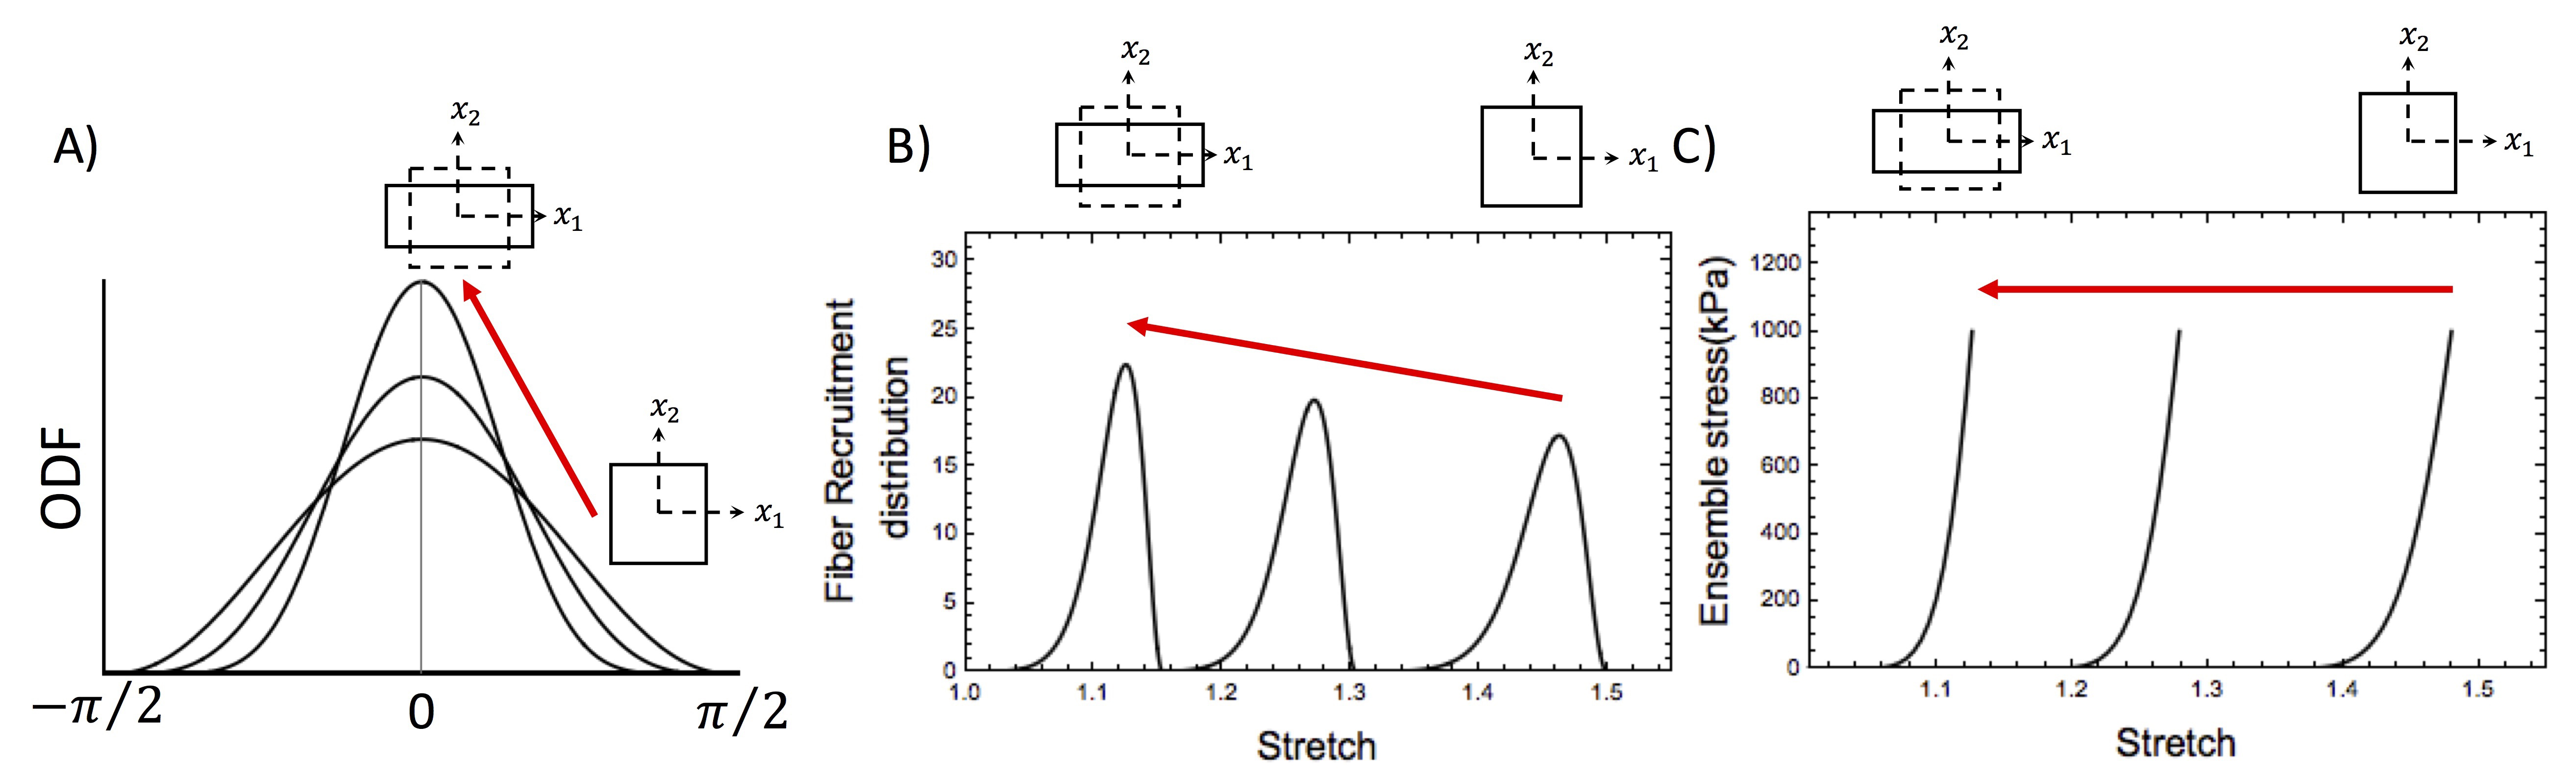
\includegraphics[width=\textwidth]{Images/chapter4/figure10}}
\caption{The effects of convecting the collagen fiber architecture show A) gradual alignment of collagen fibers, B) changes in the probability distribution of collagen fiber lack stretches and C) its effect on the mechanical response.}
\label{fig:effectsofconvection}
\end{figure}



%%%%%%%%%%%%%%%%%%%%%%%%%%%%%%%%%%%%%%%%%%%%%%%%%%%%%%%%%%%%%%%%%%%%%%%%%%%%%%%%
%%%%    Further considerations

\subsection{Further considerations of the permanent set mechanism.}

	In addition to the above considerations, we explored the the following as a means to validate the mechanisms we proposed for permanent set. This was done by performing an analysis on predicting the mechanical response after cyclic loading using only the convection of the collagen fiber architecture by the measured $\textbf{F}_{PS}$. The analysis takes the following steps: 1) Material model parameter estimation for the 0-cycle data for the strain controlled data. This is done using the approach from Sacks \textit{et al}.\cite{sacks_novel_2016}, with the constitutive model for collagen fibers and the EXL matrix from the same study, and the interaction model from equation \ref{eq:interaction}. 
	2) Use equations \ref{eq:pfODF} and \ref{eq:pfrecruitment} (Sec.\ref{sec:convection}) to convect the collagen fiber architecture (Fig. \ref{fig:structuralconvection} and Fig. \ref{fig:effectsofconvection}). 
	The deformation used to convect the collagen fiber architecture is determined from the fiducial markers. 
	3) We compare the new convected exogenously crosslinked mechanical response to the experimental data.

%\subsection{Mechanical response predicted from convected collagen fiber architecture vs experimental data after cycling}

	We used this approach to examine both the strain (n = 3) and stress controlled specimens (n = 5), and tested the hypothesis that \emph{there is a significant different between the mechanical response predicted from structural convection and the experimentally measure data}, in other words, our model is not sufficient to explain the change in mechanical response. We take the maximum stress of each specimen under equibiaxial strain, and compared the difference between the model and the experimental data using student t-test.	For the strain control specimens, we found that there is no statistical significant difference between the convected mechanical response and the experimental data, where the average p-value of the PD and XD for both after 30 million cycle and after 65 million cycle is $p = 0.37$ (minimum $p > 0.07$). 
	Likewise, we also found no statistical significant differences between the convected response and the experimental data for the stress controlled specimens, where the average p-value is 0.57 (Fig. \ref{fig:mechconvec}).
	These results suggest that 1) the underlying collagen fiber architecture, including collagen fiber crimp and orientation, is convected affinely according to the permanent set in the EXL matrix. This indicates that our approach to model permanent set is realistic, and the underlying mechanism for permanent set is likely to be correct. 
	2) Structural damage to the collagen fiber architecture was not detectable at this stage (up to 65 million cycles). 
	These important results indicate that permanent set alone is sufficient to capture the response to cyclic loading up to 50-65 million cycles. 


\begin{figure}[hbt]
\centering
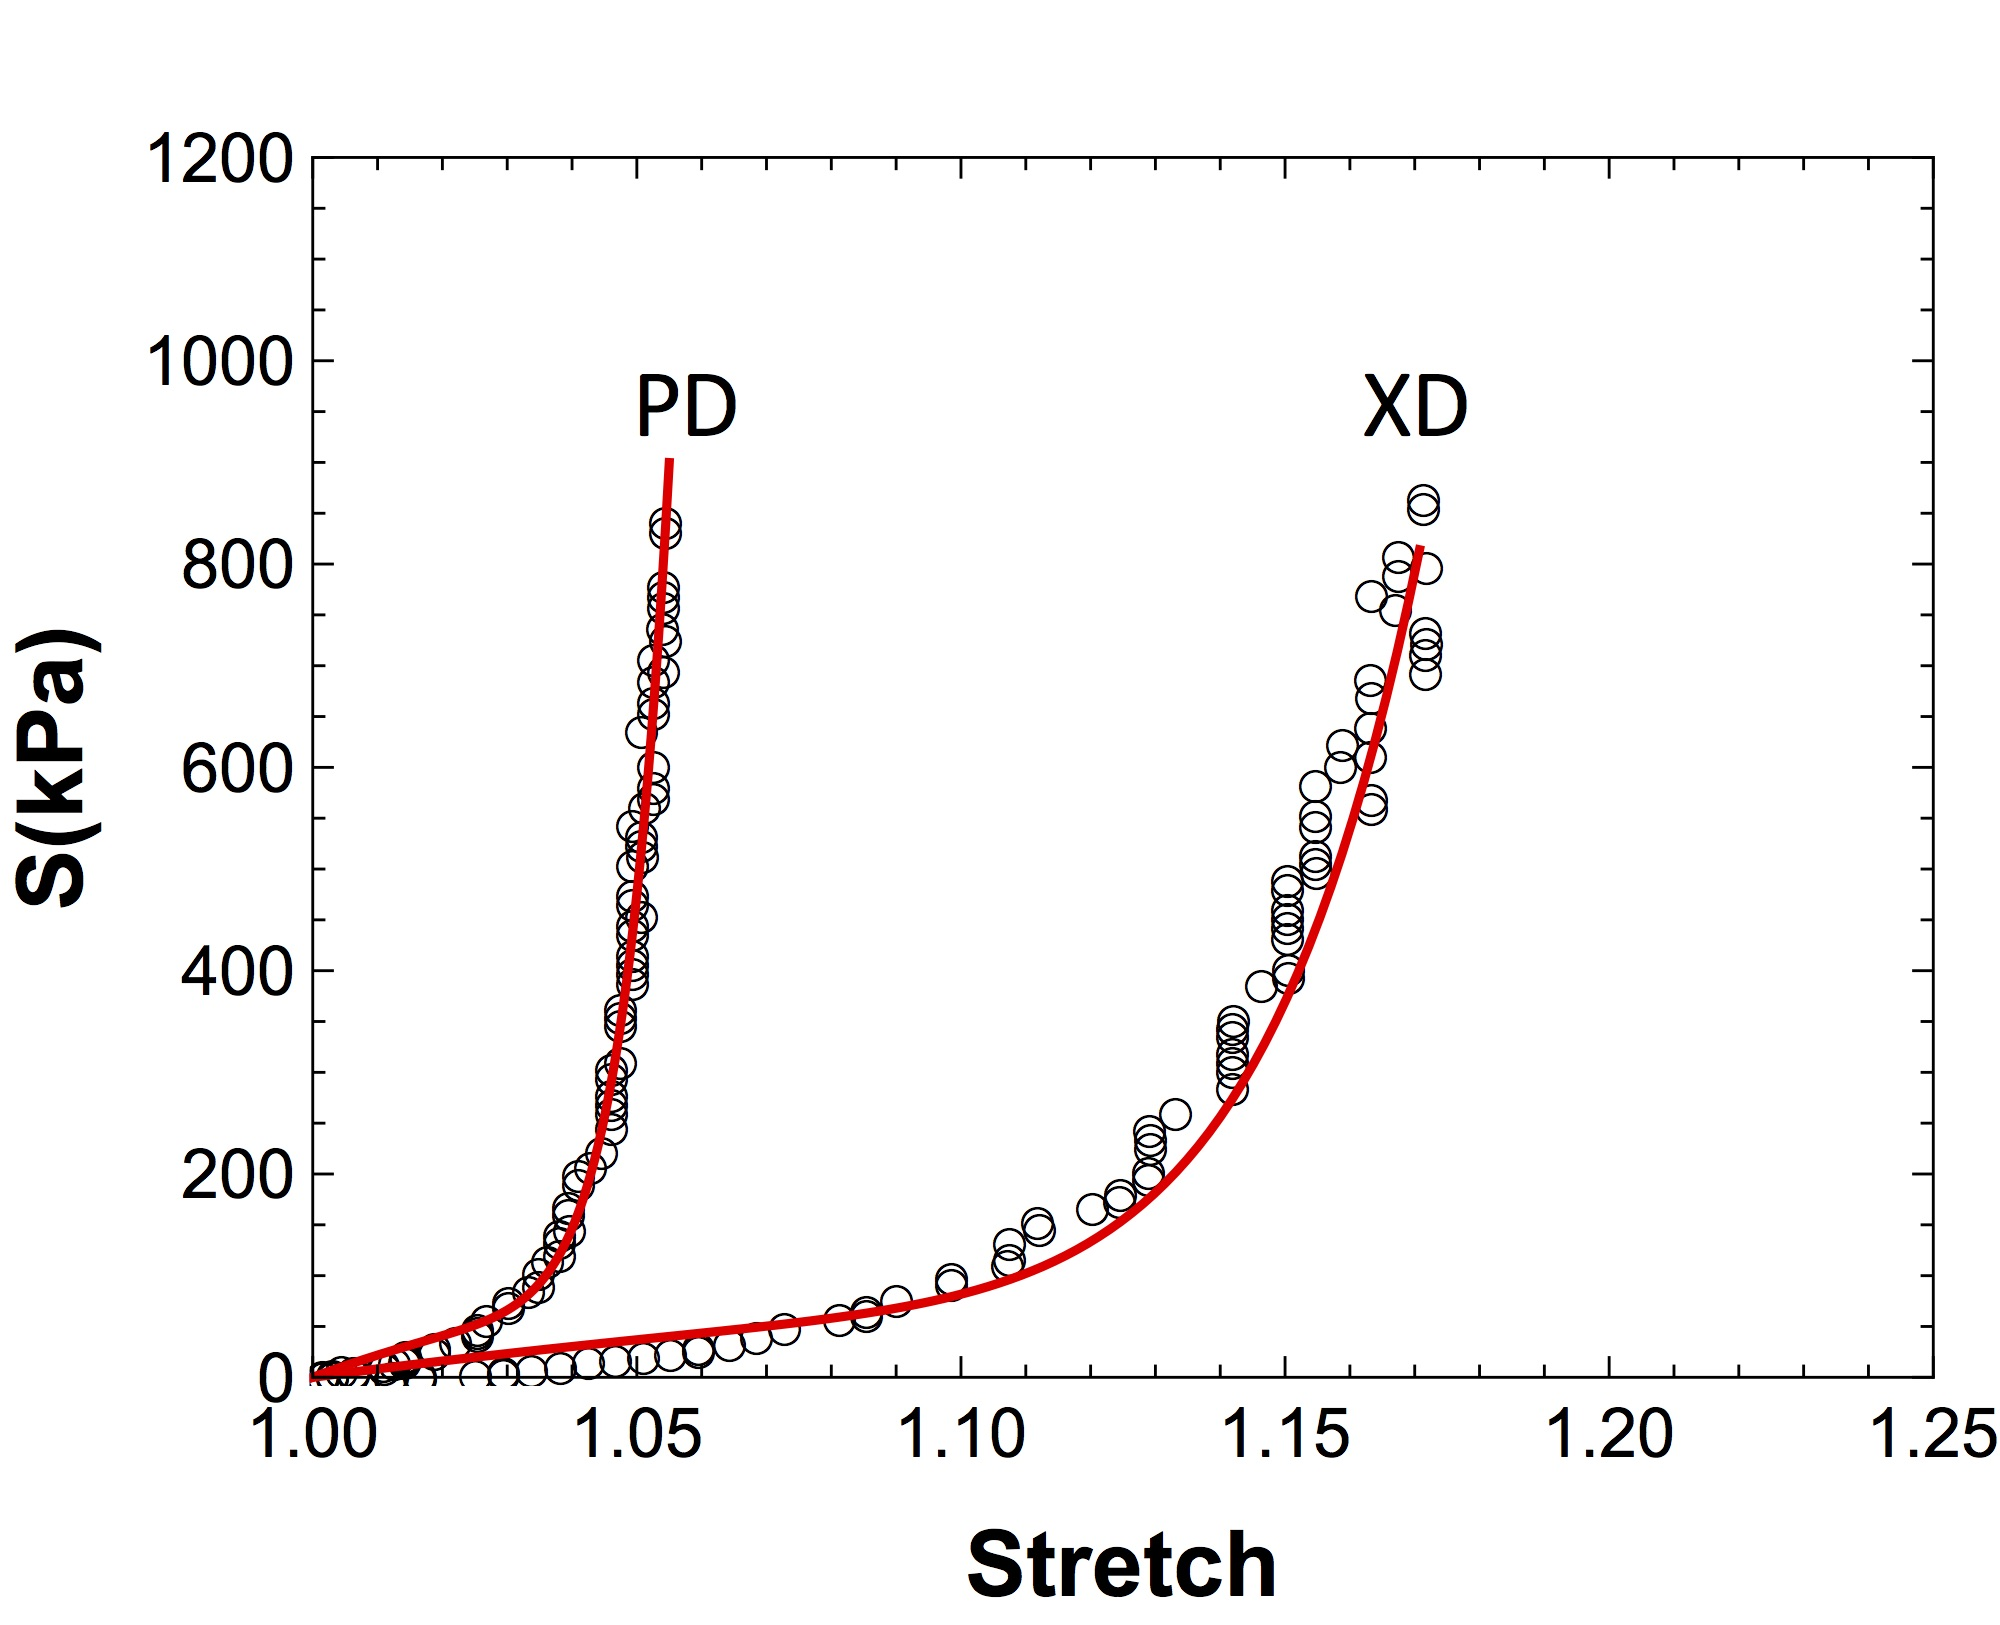
\includegraphics[width=3.5in]{Images/chapter4/figure11}
\caption{The equibiaxial mechanical response of an exogenously crosslinked BP specimen after 50 million cycles and the mechanical response determined from structural convection (Red) using the measured $\textbf{F}_{PS}$}
\label{fig:mechconvec}
\end{figure}


%%%%%%%%%%%%%%%%%%%%%%%%%%%%%%%%%%%%%%%%%%%%%%%%%%%%%%%%%%%%%%%%%%%%%%%%%%%%%%%%
%%%%    Full model form

\subsection{Full model form}
	Combining all three components, we have the final model form as a function of the permanent set rate constant $k $, the permanent set deformation $\mathbf{F}_\mathrm{PS}$, the strain history $\mathbf{A}(s)$, and the material parameters of the constitutive model in the uncycled state. The input of the model is the applied deformation $\mathbf{C}$ referenced to the current unloaded state $\Omega_\mathrm{PS}$, given by the deformation $\mathbf{F}_\mathrm{PS}$ from $\Omega_0$. The full form is
\begin{equation}\label{eq:fullEXLmodel}
\mathbf{S} = \mathbf{S}\left(k , \mathbf{F}_\mathrm{PS}, \mathbf{A}(\hat{s}), \mathbf{C}\right) = \phi_\mathrm{col} \left[ \mathbf{S}_\mathrm{col} + \mathbf{S}_\mathrm{int}\right] + \phi_m \mathbf{S}_\mathrm{m},
\end{equation}
where the collagen contribution is 
\begin{equation} \label{eq:fullcollagen}
\begin{split}
\phi_\mathrm{col}\mathbf{S}_\mathrm{col}\left(k , \mathbf{F}_\mathrm{PS}, \mathbf{A}(\hat{s}), \mathbf{C}\right) =& \phi_\mathrm{col} \eta_C \int\displaylimits_\theta \Gamma_1(\mathbf{F}_{\mathrm{PS}}, \theta)\left\lbrace 
\int\displaylimits_1^{\lambda_\theta} \frac{D_1\left( \mathbf{F}_{\mathrm{PS}}, x \right)}{x} \left( \frac{1}{x}- \frac{1}{\lambda_\theta}\right) \mathrm{d}x \right\rbrace \mathbf{n}_\theta\otimes\mathbf{n}_\theta \mathrm{d}\theta,
\end{split}
\end{equation}
where $\lambda_\theta = \sqrt{\mathbf{n}_\theta \cdot \mathbf{C}\mathbf{n}_\theta}$ is the stretch of the fiber ensemble oriented along $\theta$, the fiber ensemble interactions is 
\begin{equation} \label{eq:fullinteractions}
\begin{split}
\phi_\mathrm{int}\mathbf{S}_\mathrm{int}\left(k , \mathbf{F}_\mathrm{PS}, \mathbf{A}(\hat{s}), \mathbf{C}\right) = \phi_\mathrm{col} \eta_\mathrm{int}& \int\displaylimits_\alpha \int\displaylimits_\beta \Gamma_1 \left(\mathbf{F}_\mathrm{PS}, \alpha \right) \Gamma_1 \left(\mathbf{F}_\mathrm{PS},  \beta \right) \\
\times&\left[ \left\lbrace 
\int\displaylimits_1^{\lambda_\alpha} \int\displaylimits_1^{\lambda_\beta} 
\frac{2 \lambda_\beta D_1(\mathbf{F}_\mathrm{PS}, x_\alpha) D_1(\mathbf{F}_\mathrm{PS}, x_\beta)}{x_\alpha x_\beta} 
\left( \frac{\lambda_\alpha}{x_\alpha} \frac{\lambda_\beta}{x_\beta} - 1\right) \mathrm{d}x_\alpha \, \mathrm{d}x_\beta \right.\right. \\
+& \left. \left. \int\displaylimits_1^{\lambda_\beta} D_1(\mathbf{F}_\mathrm{PS}, x_\beta) \left( \frac{\lambda_\beta}{x_\beta} -1  \right)^2 \mathrm{d}x_\beta \right\rbrace \right.  \frac{\mathbf{n}_\alpha \otimes \mathbf{n}_\alpha}{\lambda_\alpha}  \\
+& \left. \left\lbrace
\int\displaylimits_1^{\lambda_\alpha} \int\displaylimits_1^{\lambda_\alpha} 
\frac{2 \lambda_\beta D_1(\mathbf{F}_\mathrm{PS}, x_\alpha) D_1(\mathbf{F}_\mathrm{PS}, x_\beta)}{x_\alpha x_\beta} 
\left( \frac{\lambda_\alpha}{x_\alpha} \frac{\lambda_\beta}{x_\beta} - 1\right) \mathrm{d}x_\alpha \, \mathrm{d}x_\beta 
\right. \right. \\
+&\left. \left. \int\displaylimits_1^{\lambda_\alpha} D_1(\mathbf{F}_\mathrm{PS}, x_\alpha) \left( \frac{\lambda_\alpha}{x_\alpha} -1  \right)^2 \mathrm{d}x_\alpha \right\rbrace \frac{\mathbf{n}_\beta \otimes \mathbf{n}_\beta}{\lambda_\beta}  \right] \mathrm{d}\alpha \, \mathrm{d}\beta,
\end{split}
\end{equation}
and the EXL matrix is
\begin{equation} \label{eq:fullmatrix}
\begin{split}
\phi_m \mathbf{S}_\mathrm{m}\left(k , \mathbf{F}_\mathrm{PS}, \mathbf{A}(\hat{s}), \mathbf{C}\right) = \phi_m \eta_m& \left[ \vphantom{\int\displaylimits_0^s} \mathrm{Exp}\left[-k  \cdot s\right]  \left(\left( \bar{I_1} (\mathbf{F}_\mathrm{PS}, \mathbf{A}(0)) - 3\right)^{\alpha - 1} + r \left( \bar{I_1} (\mathbf{F}_\mathrm{PS}, \mathbf{A}(0)) - 3\right)^{\beta - 1}\right)  \right.\\
\times& \left( \mathbf{\tilde{B}}(\mathbf{F}_\mathrm{PS}, \mathbf{A}(0))^{-1} - \tilde{B}_{33}^{-1}(\mathbf{F}_\mathrm{PS}, \mathbf{A}(0))C_{33}\mathbf{C}^{-1}\right) \\
+& \int\displaylimits_0^s k \cdot \mathrm{Exp}\left[-k (s - \hat{s})\right] \left(\left( \bar{I_1} (\mathbf{F}_\mathrm{PS}, \mathbf{A}(\hat{s})) - 3\right)^{\alpha - 1} + r \left( \bar{I_1} (\mathbf{F}_\mathrm{PS}, \mathbf{A}(\hat{s})) - 3\right)^{\beta - 1}\right) \\
\times& \left. \vphantom{\int\displaylimits_-^s} \left( \mathbf{\tilde{B}}(\mathbf{F}_\mathrm{PS}, \mathbf{A}(\hat{s}))^{-1} - \tilde{B}_{33}^{-1}(\mathbf{F}_\mathrm{PS}, \mathbf{A}(\hat{s}))C_{33}\mathbf{C}^{-1}\right) \mathrm{d}\hat{s}\right].
\end{split}
\end{equation}

%%%%%%%%%%%%%%%%%%%%%%%%%%%%%%%%%%%%%%%%%%%%%%%%%%%%%%%%%%%%%%%%%%%%%%%%%%%%%%%%
%%%%    Finding permanent set deformations

\subsection{Determining permanent set deformation and loaded state}
To solve for the permanent set deformation ($\mathbf{F}_\mathrm{PS}$), and for the deformation ($\mathbf{A}(s)$) to the new loaded state after permanent set ($\Omega(s)$) when under an applied stress of $\mathbf{\hat{S}}$, we need to use optimization as the permanent set constitutive model has no analytical inverse form. Specifically,
\begin{equation}\label{eq:optimization}
\begin{gathered}
\mathbf{F}_\mathrm{PS} = \operatorname*{arg\,min}_\mathbf{F} \left\Vert \mathbf{S}\left(k , \mathbf{I}, \mathbf{A}(\hat{s}), \mathbf{C}=\mathbf{F}^\mathsf{T}\mathbf{F}\right) - 0 \right\Vert, \\
\mathbf{A}(s) = \operatorname*{arg\,min}_\mathbf{F} \left\Vert \mathbf{S}\left(k , \mathbf{I}, \mathbf{A}(\hat{s}), \mathbf{C}=\mathbf{F}^\mathsf{T}\mathbf{F}\right) - \mathbf{\hat{S}} \right\Vert.
\end{gathered}
\end{equation}

%%%%%%%%%%%%%%%%%%%%%%%%%%%%%%%%%%%%%%%%%%%%%%%%%%%%%%%%%%%%%%%%%%%%%%%%%%%%%%%%
%%%%    Modeling and parameter estimation

\subsection{Modeling approach and parameter estimation}

%%%%%%%%%%%%%%%%%%%%%%%%%%%%%%%%%%%%%%%%%%%%%%%%%%%%%%%%%%%%
%%%%    Strain controlled cycling

\subsubsection{Strain controlled cycling}
	Our goal using the strain controlled data is to validate the constitutive model form and perform parameter estimation. Since the loaded state never changes, the permanent set model can be simplified into a two-state model, with the loaded state ($\Omega(s)$) being the root mean square strain. Specifically, the EXL matrix can be simplified to
\begin{equation} 
\begin{split}
\phi_m \mathbf{S}_m &= \phi_m \left[ \mathrm{Exp}\left[-k  \cdot s\right] \mathbf{\bar{S}}_m \left(\mathbf{F}_\mathrm{PS}, \mathbf{I},\mathbf{C}\right) + \int\displaylimits_0^s k \cdot  \mathrm{Exp}\left[-k (s - \hat{s})\right] \mathbf{\bar{S}}_m \left(\mathbf{F}_\mathrm{PS}, \mathbf{A},\mathbf{C}\right) \mathrm{d}\hat{s} \right] \\
&= \phi_m \left[ \mathrm{Exp}\left[-k  \cdot s\right] \mathbf{\bar{S}}_m \left(\mathbf{F}_\mathrm{PS}, \mathbf{I},\mathbf{C}\right) + \left(1 - \mathrm{Exp}\left[-k  \cdot s\right] \right) \mathbf{\bar{S}}_m \left(\mathbf{F}_\mathrm{PS}, \mathbf{A},\mathbf{C}\right) \right].
\end{split}
\end{equation}
Of the 3 time points (0, 30, and 65 million cycles), we fit the first two time points (0 and 30 million cycles) and use the results to predict the response to cycling at 65 million cycles as a way to validate our model (Fig. \ref{fig:datamethods}A). We note that the mounted configuration of the specimen for mechanical testing and cyclic loading are not the same, thus there is a small rigid body rotation of the specimen between the two testing configurations. We will compensate for this during the parameter estimation, which is done as followed
\begin{enumerate}
\item Determine the 0-cycled mechanical response using the methods of Sacks \textit{et al}.\cite{sacks_novel_2016}
\item Fit the permanent set deformation $\mathbf{F}_\mathrm{PS}$ and the mechanical response at the same time for the 30 million cycles time point
	\begin{enumerate}
	\item choose a $k $
	\item choose a mounting direction $\theta_\mathrm{mount}$
	\item compute $err_\mathrm{PS} = \mathbf{F}_\mathrm{PS} - \mathbf{F}_\mathrm{PS}^\mathrm{data}$ error at 30 million cycles
	\item compute $err_\mathrm{\mathbf{S}} = \mathbf{S}^\mathrm{max} - \mathbf{S}_\mathrm{data}^\mathrm{max}$
	\item compute the weighted error $err_\mathrm{PS} + W_\mathbf{S} err_\mathbf{S}$, where the weight $W_\mathbf{S} = $max strain in the direction of loading/$\mathbf{S}_\mathrm{data}^\mathrm{max}$
	\item update $k $ and $\theta_\mathrm{mount}$ using the Quasi-Newton method \cite{king_dlib_2009}
	\end{enumerate}
\item Predict $\mathbf{F}_\mathrm{PS}$ and the mechanical response at 65 million cycles
\end{enumerate}


\begin{figure}[hbt]
\centering
\centerline{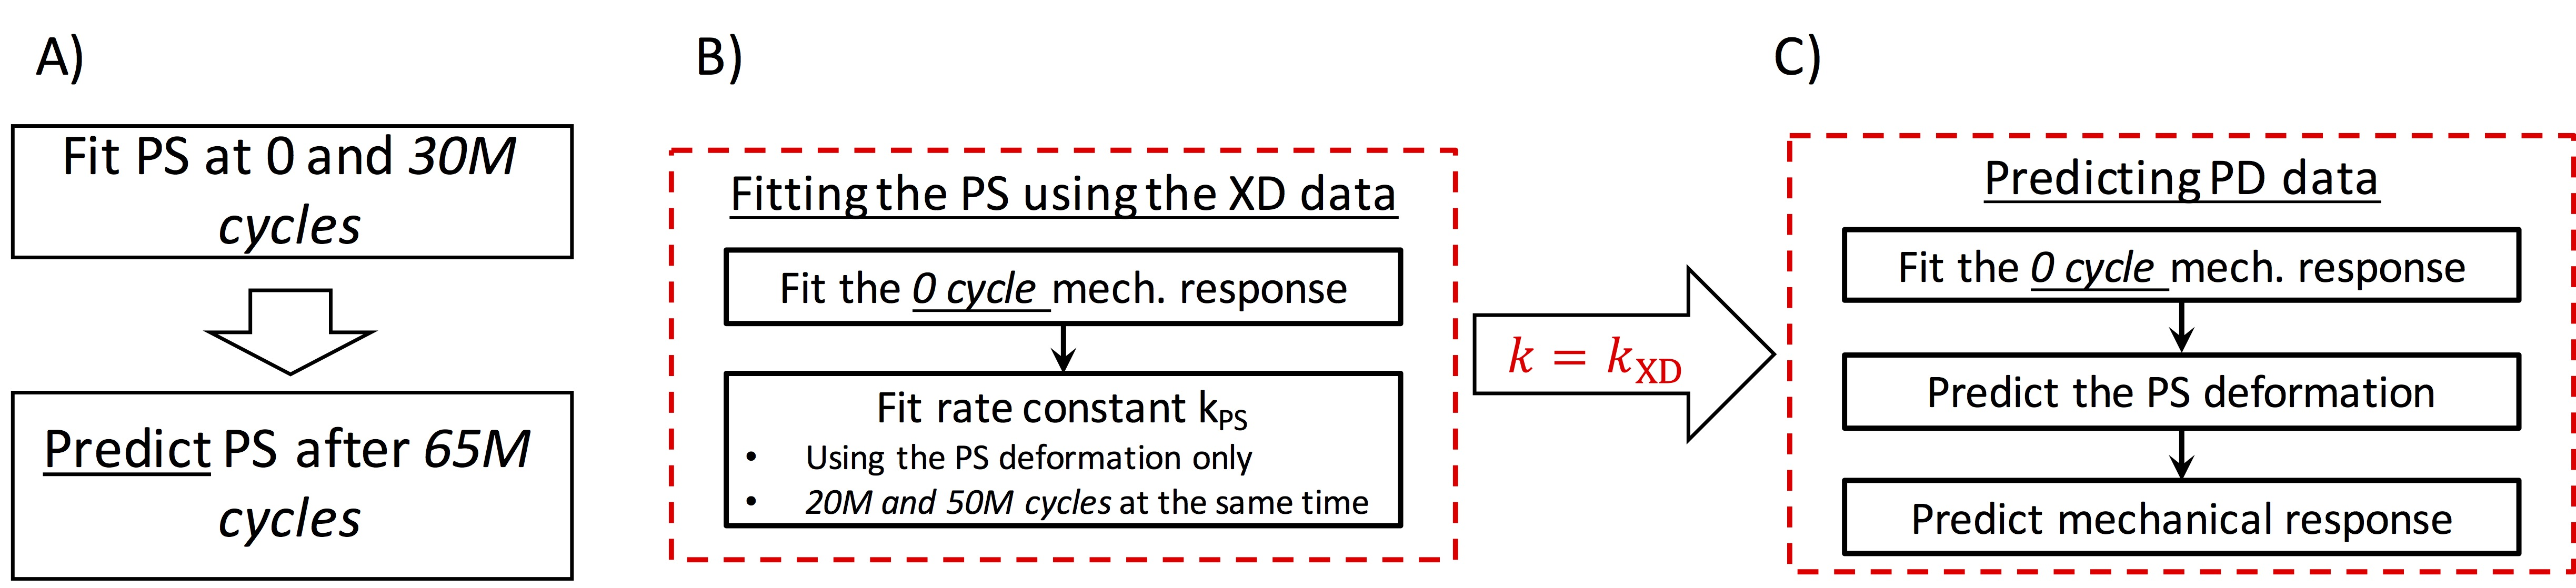
\includegraphics[width=\textwidth]{Images/chapter4/figure12}}
\caption{Our parameter estimation approach for the A) strain controlled cyclic loading data, B) stress controlled data cycled in the cross-preferred direction and C) in the preferred direction}
\label{fig:datamethods}
\end{figure}


%%%%%%%%%%%%%%%%%%%%%%%%%%%%%%%%%%%%%%%%%%%%%%%%%%%%%%%%%%%%
%%%%    Stress controlled cycling

\subsubsection{Stress controlled cycling}
The parameter estimation for the stress controlled specimens is more complicated than the strain controlled specimens as we do not know the strain history \textit{a priori}. This becomes a dynamic simulation, and we need to use optimization to determine the strain history (Eqn. \ref{eq:optimization}) at each time point. Thus, this data set is well suited to validate the full model using time dependent simulations. Since we have data for both PD-loading and XD-loading, we can fit the XD-loading data and used the resulting rate constant $k $ to predict the PD-loading data. First, we discretized the problem as followed
\begin{equation} 
\begin{aligned}
\phi_m \mathbf{S}_m =& \phi_m \left[\mathrm{Exp} \left[-k  \cdot n \cdot \Delta s \right] \mathbf{\bar{S}}_m \left(\mathbf{F}_\mathrm{PS}, \mathbf{I},\mathbf{C}\right)\vphantom{\sum_{i = 1}^n}\right. \\
&+ \left.\sum_{i = 1}^n  (k \Delta s) \mathrm{Exp}\left[-k (n\Delta s - i \Delta s)\right] \mathbf{\bar{S}}_m \left(\mathbf{F}_\mathrm{PS}, \mathbf{A}(i\Delta s),\mathbf{C}\right)\right].
\end{aligned}
\end{equation}
After each time step $\Delta s$, we compute the new loaded state $\mathbf{A}(i\Delta s)$ using optimization(Eqn. \ref{eq:optimization}, Fig. \ref{fig:implementation}). Through preliminary trials, the most optimal resolution in time is $\Delta s = 1$ million cycles when considering both time to run the simulations and accuracy of the results. We note that since an additional optimization is added to the parameter estimation process, we can no longer fit both the permanent set deformation $\mathbf{F}_\mathrm{PS}$ and the mechanical data at the same time. Our attempts at fitting both at the same time were not able to converge. Thus, we choose to predict the mechanical data as a way to validate our results. 
The parameter estimation process for the XD-loading data is
\begin{enumerate}
\item Determine the 0-cycled mechanical response
\item Fit the permanent set deformation $\mathbf{F}_\mathrm{PS}$ 
	\begin{enumerate}
	\item choose a $k $
	\item choose a mounting direction $\theta_\mathrm{mount}^{20}$ for cycling up to 20 million cycles 
	\item compute $err_\mathrm{PS} = \mathbf{F}_\mathrm{PS} - \mathbf{F}_\mathrm{PS}^\mathrm{data}$ error at 20 million cycles
	\item choose a mounting direction $\theta_\mathrm{mount}^{50}$ for cycling from 20 to 50 million cycles 
	\item compute $err_\mathrm{PS} = \mathbf{F}_\mathrm{PS} - \mathbf{F}_\mathrm{PS}^\mathrm{data}$ error at 50 million cycles
	\item update $k$, $\theta_\mathrm{mount}^{20}$, and $\theta_\mathrm{mount}^{50}$ using Quasi-Newton
	\end{enumerate}
\item Predict the mechanical response 
\end{enumerate}
Next we, used $k $ from the XD-loading data to predict the PD-loading data. 
\begin{enumerate}
\item Determine the 0-cycled mechanical response
\item Compute Fit the permanent set deformation $\mathbf{F}_\mathrm{PS}$
	\begin{enumerate}
	\item set $k $ from XD-loading data
	\item choose a mounting direction $\theta_\mathrm{mount}^{20}$ for cycling up to 20 million cycles 
	\item compute $err_\mathrm{PS} = \mathbf{F}_\mathrm{PS} - \mathbf{F}_\mathrm{PS}^\mathrm{data}$ error at 20 million cycles
	\item choose a mounting direction $\theta_\mathrm{mount}^{50}$ for cycling from 20 to 50 million cycles 
	\item compute $err_\mathrm{PS} = \mathbf{F}_\mathrm{PS} - \mathbf{F}_\mathrm{PS}^\mathrm{data}$ error at 50 million cycles
	\item update $\theta_\mathrm{mount}^{20}$ and $\theta_\mathrm{mount}^{50}$ using Quasi-Newton
	\end{enumerate}
\item Predict the mechanical response 
\end{enumerate}

%%%%%%%%%%%%%%%%%%%%%%%%%%%%%%%%%%%%%%%%%%%%%%%%%%%%%%%%%%%%%%%%%%%%%%%%%%%%%%%%
%%%%    Parametric studies


\begin{figure}[hbt]
\centering
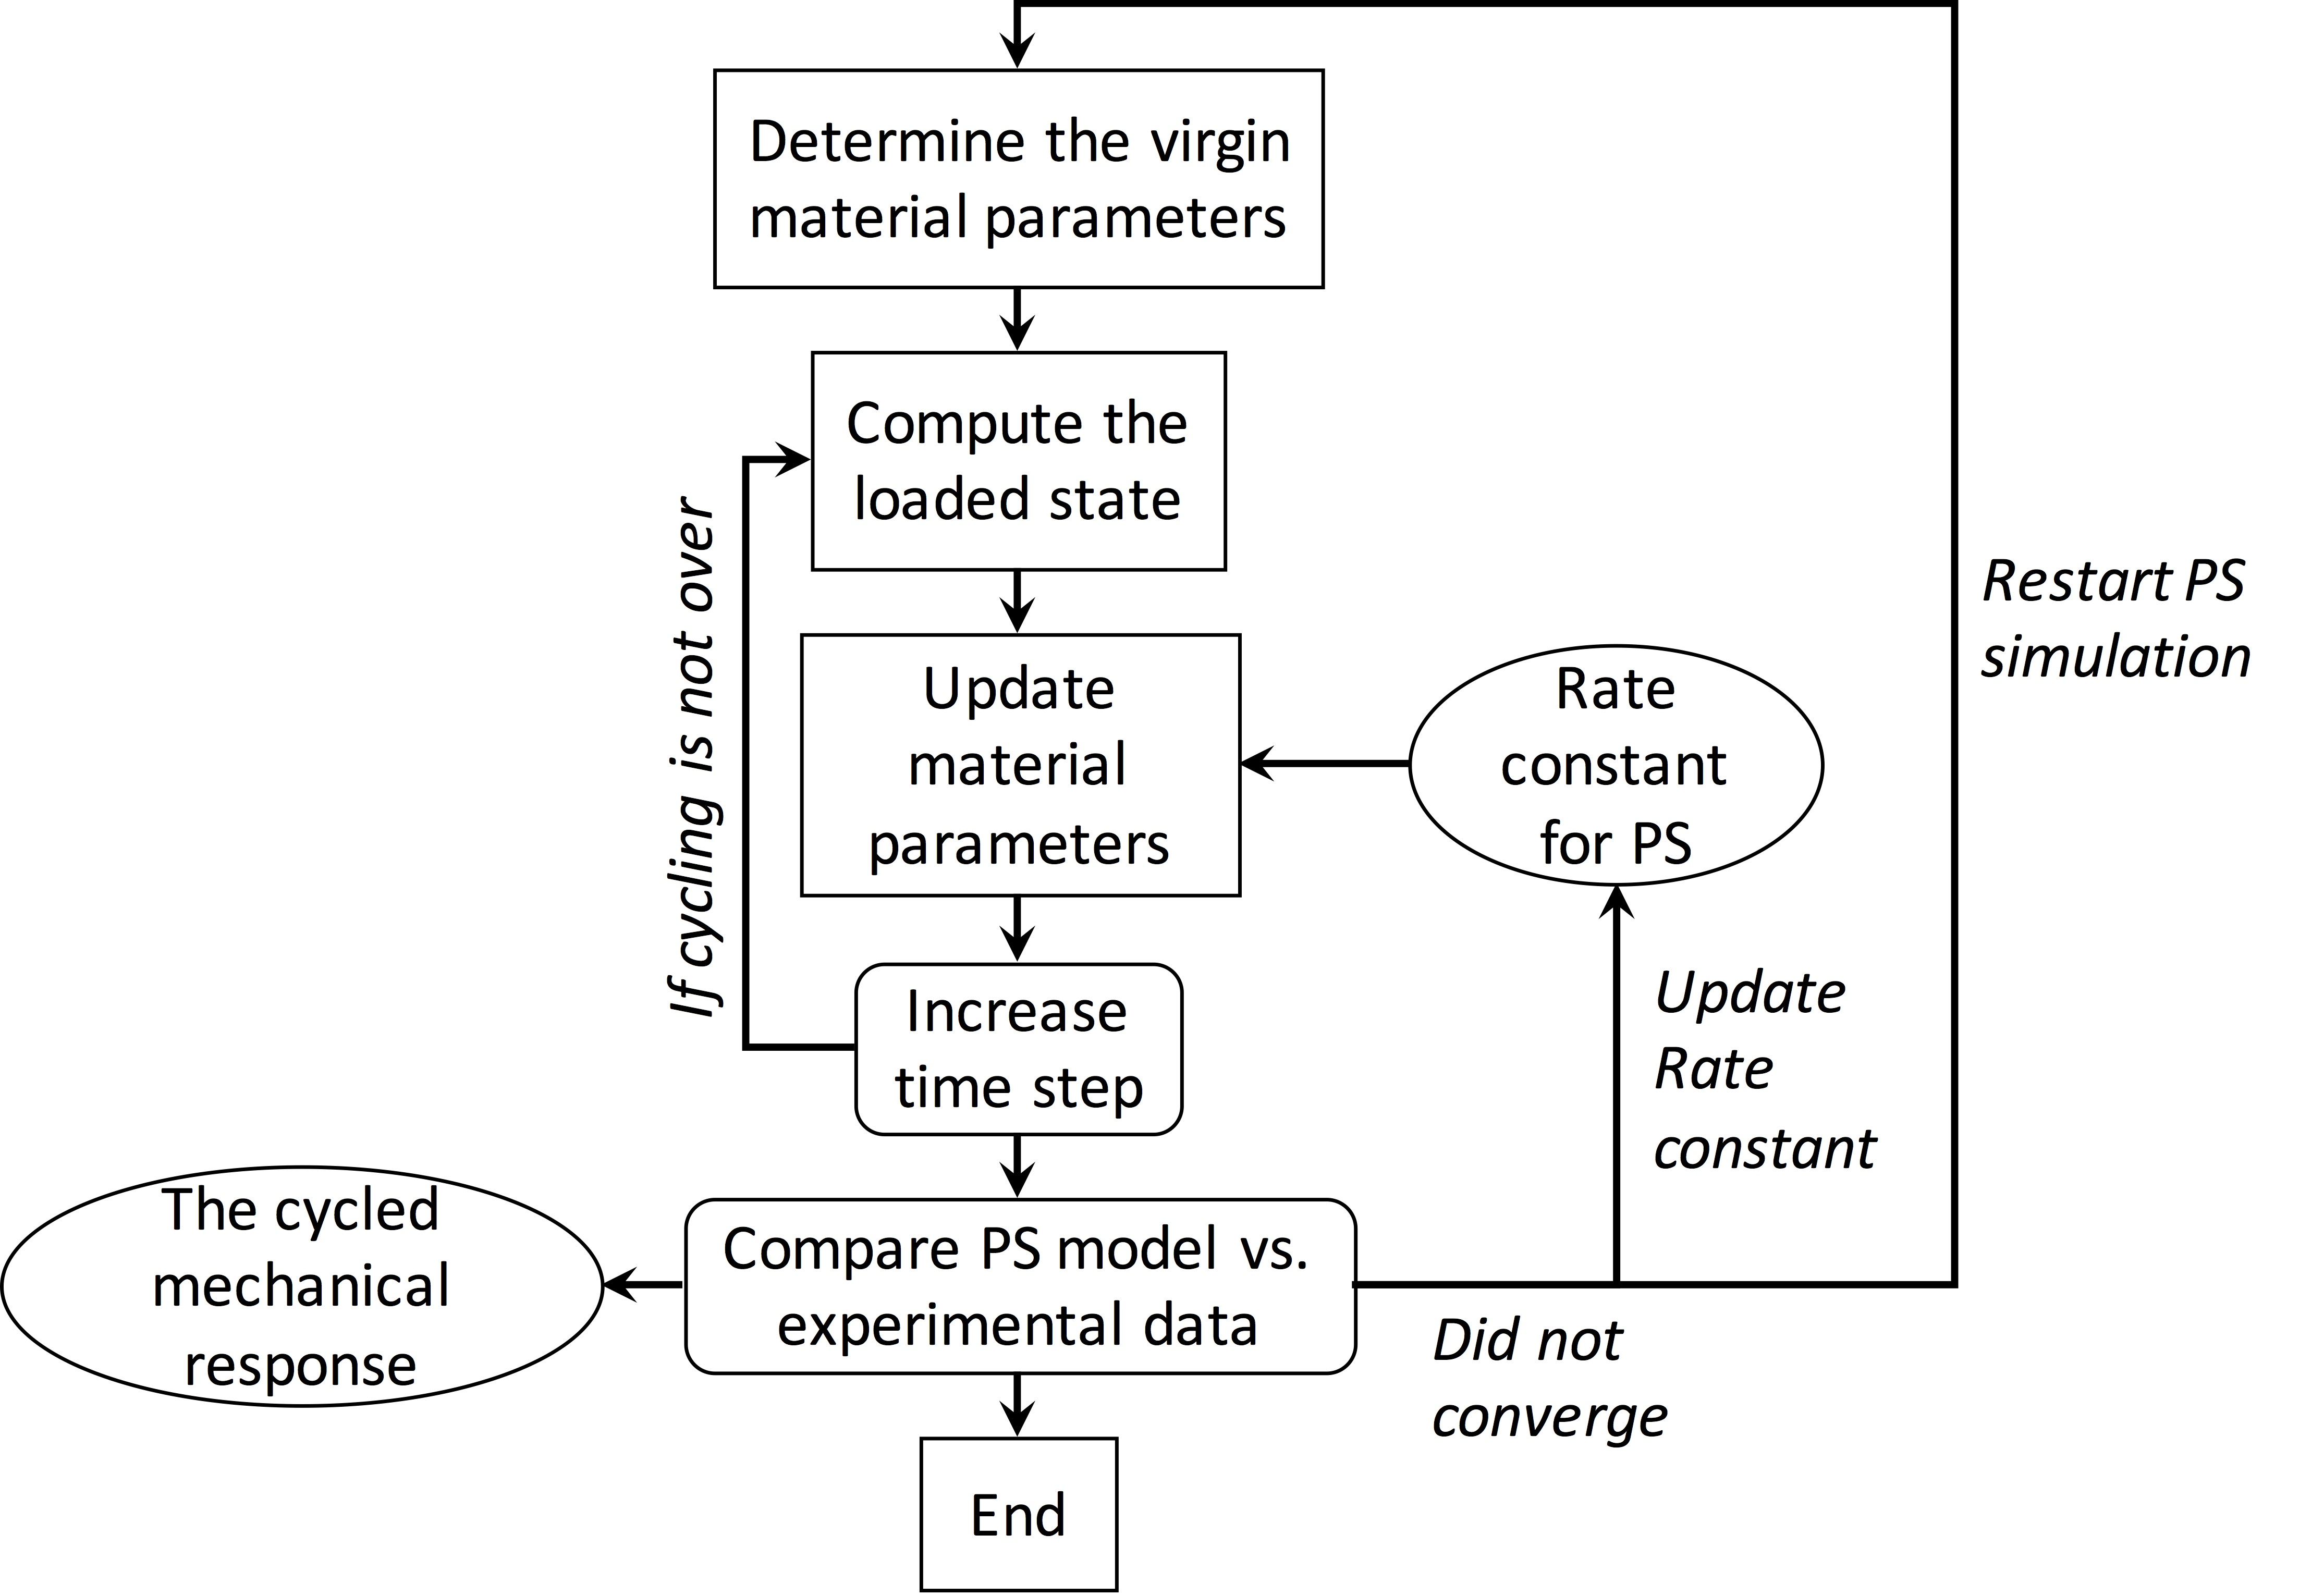
\includegraphics[width=5in]{Images/chapter4/figure13}
\caption{Implementation of the full model with updates in time.}
\label{fig:implementation}
\end{figure}


\subsection{Parametric studies}
Next, we performed an parametric study using the stress-controlled PD data. The same material parameters and rate constant, $k$, from parameter estimation results above was used. We simulated one specimen by extending the cycle duration to 100 million cycles to examine how the changes in geometry due to permanent set respond to an extended cycling period. 

%---    primary results
\section{Permanent set model results}
\subsection{Model fit and predictive capabilities}


	For the strain control specimens, we found that we were able to fit the permanent set deformations very well ($R^2 = 0.96$) (Fig. \ref{fig:strainresults}A). We were able to predict the mechanical response of the strain controlled specimens at 65 million cycles ($R^2 = 0.83$) (Fig. \ref{fig:strainresults}B\&C). 
	For the stress controlled specimens, we found we were able to fit the permanent set deformations for the XD specimens ($R^2 = 0.93$)(Fig. \ref{fig:stressXDdef}B), as well as predict the PD specimens very well ($R^2 = 0.97$) (Fig. \ref{fig:stressXDdef}C). 
	The resulting rate constant from both data sets shown no statistical difference ($p > 0.98$)(Fig. \ref{fig:stressXDdef}A). 
The mechanical response for the stress controlled XD specimens did not match as well in terms of the $R^2$ value($R^2 = 0.72$). 
	However, given none of the mechanical data was involved in the parameter estimate this was nevertheless a very good prediction. 
	For example, when comparing the model to the experimental data by extrapolating the loading path of the equibiaxial protocol and finding the peak strain at 1MPa, the $R^2$ value increases to 0.93. 
	One the other hand, the predicted mechanical response for the PD controlled data were very good ($R^2 = 0.95$) (Fig. \ref{fig:stressPDmech}), suggesting that our model was able to capture the underlying mechanisms. 
	These results agree with our hypothesis that the initial changes in the mechanical response (in the first 50 million cycles) can be predicted by the change in microstructure alone, and that structural damage is low at this stage. 
\begin{figure}[hbt]
\centering
\centerline{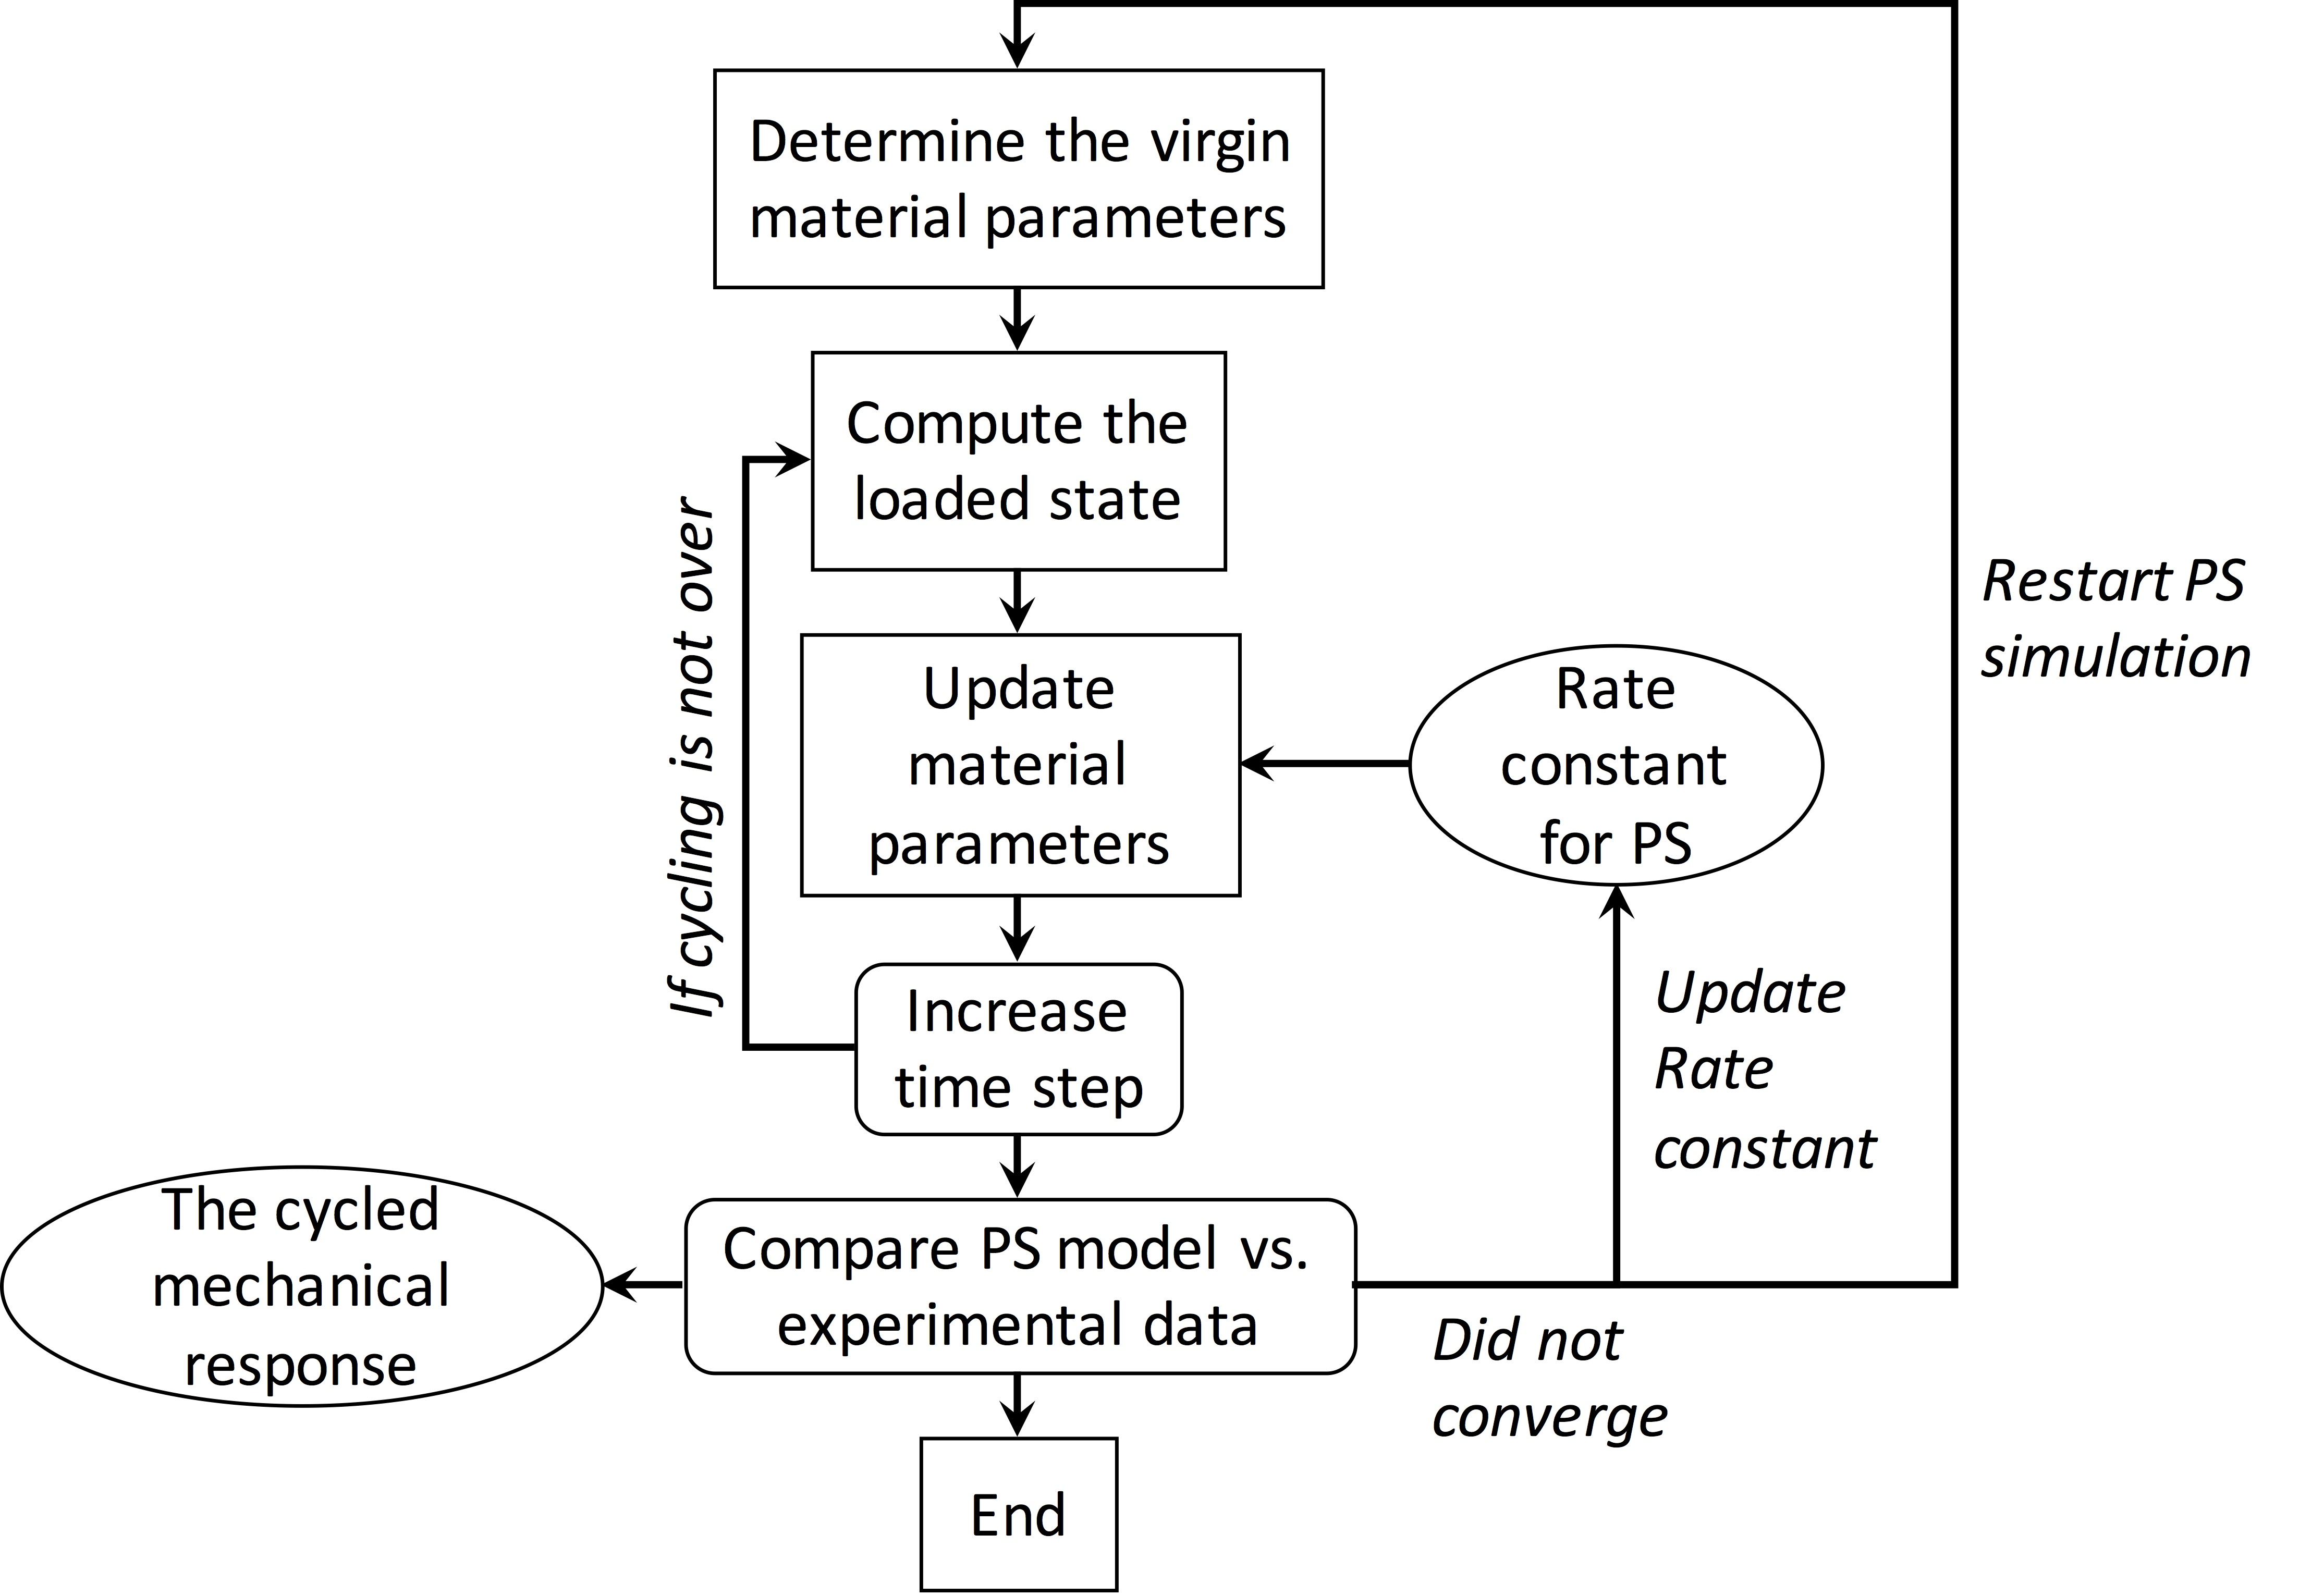
\includegraphics[width=0.75\paperwidth]{Images/chapter4/figure13}}
\caption{Results of the strain controlled cycling data, shown how the A) model fits the permanent set deformation at 30 million cycles and predicts the 65 million cycles time point(in box), as well as C) how the model predicts the mechanical response at 65 million cycles using material parameters from the B) 0 cycle time point.}
\label{fig:strainresults}
\end{figure}
\begin{figure}[hbt]
\centering
\centerline{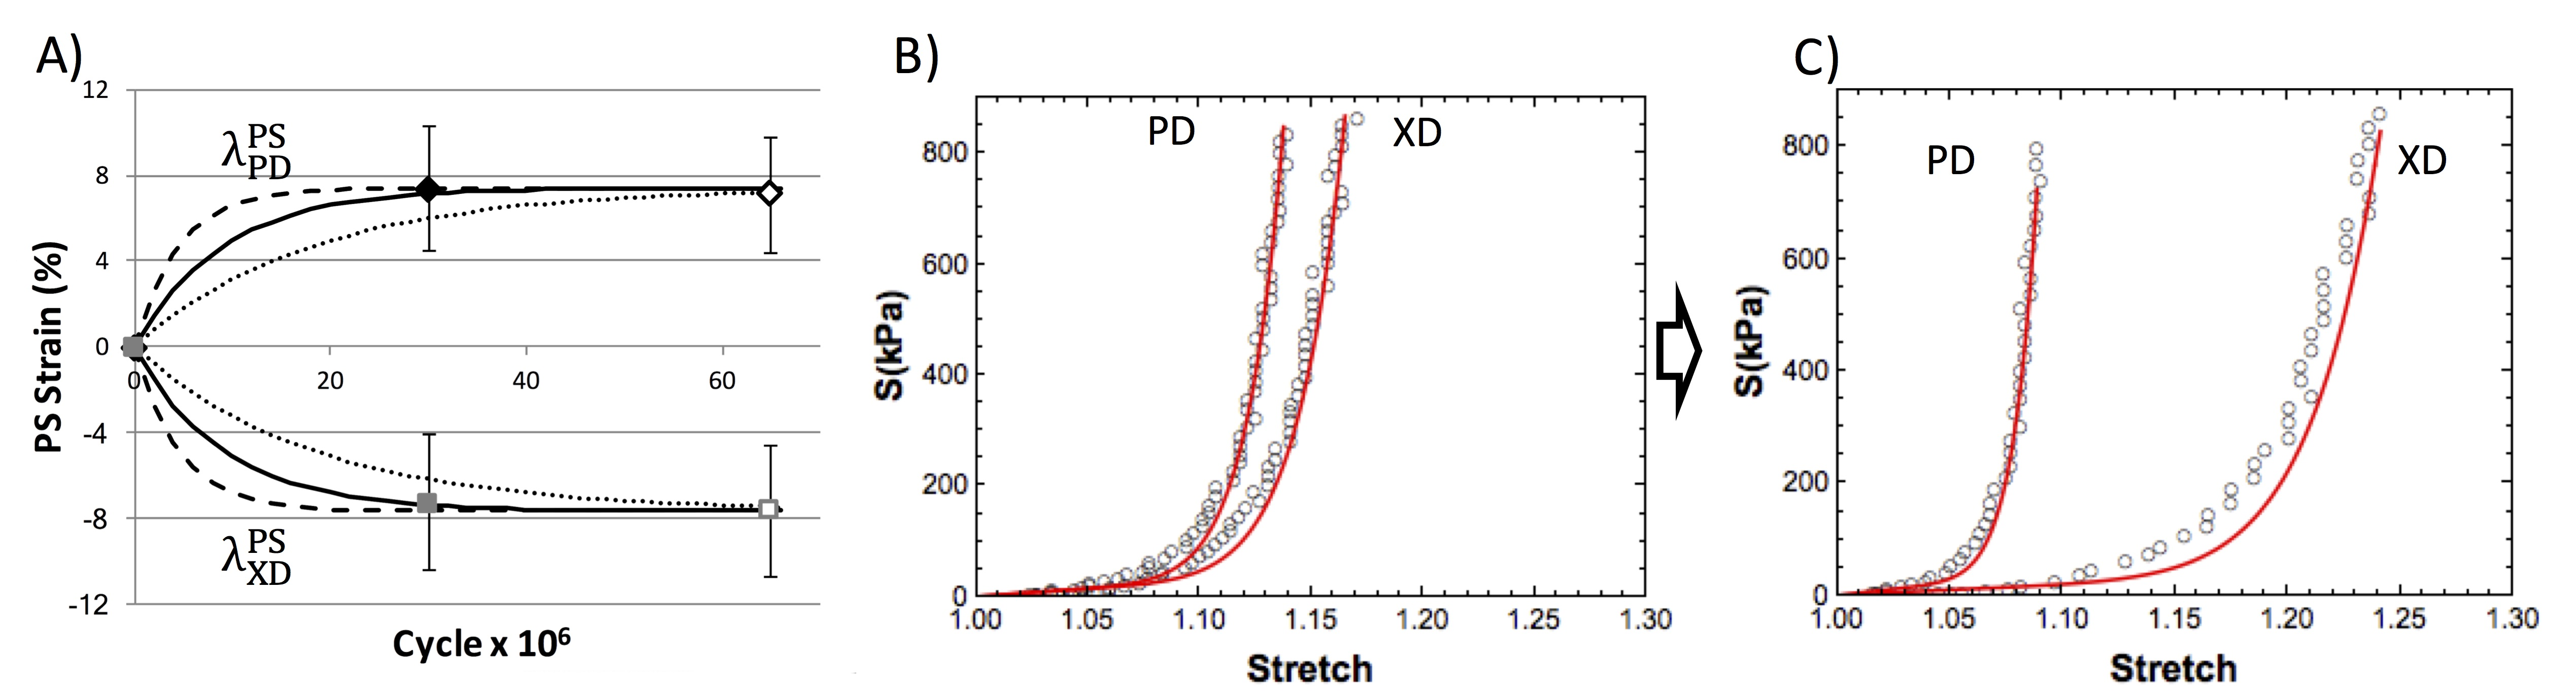
\includegraphics[width=0.75\paperwidth]{Images/chapter4/figure14}}
\caption{A) The model fit for the permanent set deformation at both 20 and 50 million cycles for the stress controlled XD cycled specimens. B) Comparison of the permanent set rate constant between the strain controlled and stress controlled specimens. C) The predicted permanent set deformation for the PD cycled specimens using the rate constant from fitting the XD cycled specimens. }
\label{fig:stressXDdef}
\end{figure}
\begin{figure}[hbt]
\centering
\centerline{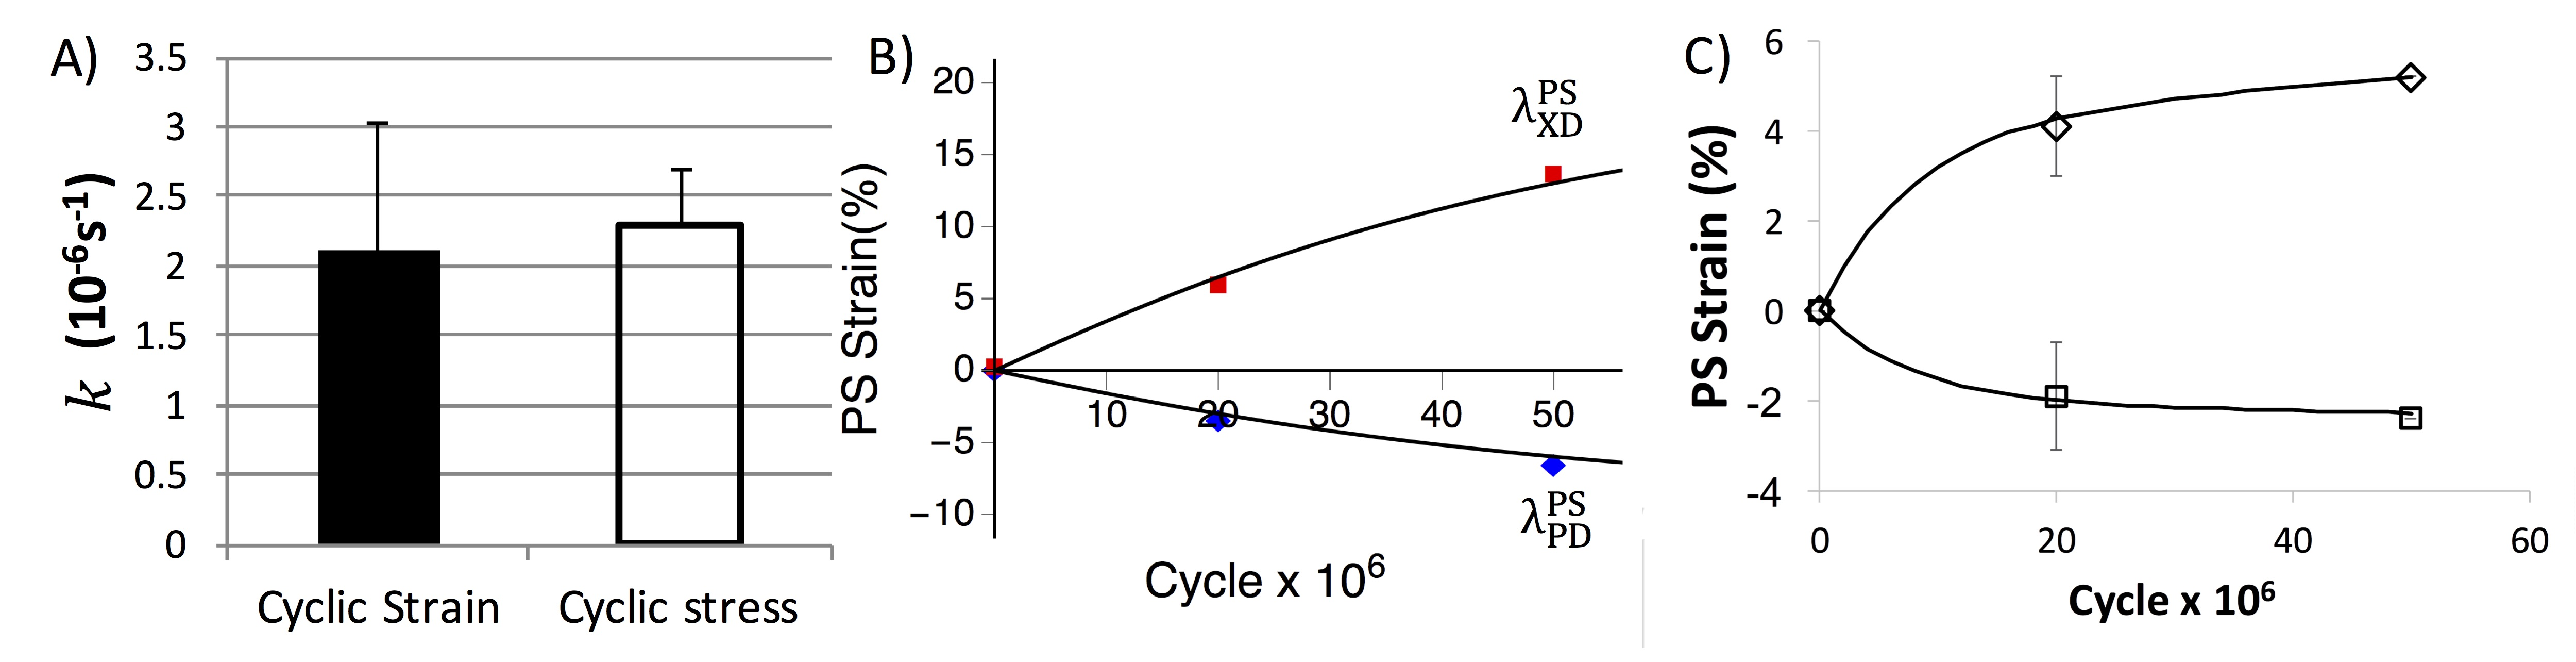
\includegraphics[width=0.75\paperwidth]{Images/chapter4/figure15}}
\caption{A) Best fit of the mechanical response at 0 cycle for the material parameters ($r^2 = 0.98$). The predicted mechanical response for the representative PD cycled specimen at B) 20 ($r^2 = 0.87$) and C) 50 million cycles. ($r^2 = 0.82$)}
\label{fig:stressPDmech}
\end{figure}

\subsection{Parametric study results}
	By extending the cycling duration in the parametric study, we found that the permanent set deformation reaches an assymptote after approximately 70 million cycles when loading along the PD. 
	This threshold slightly exceeds the lower bound for collagen recruitment. 
	We estimate that around 2.6\% of collagen fiber are recruited when the permanent set deformation reaches this threshold (Fig. \ref{fig:parametric}). 
	This suggests that collagen fibers are limiting the maximum change in geometry that can occur, and that the lower bound of the collagen fiber recruitment can serve as an estimated bound for the change in geometry due to the permanent set effect in BHVs, as collagen fibers start resisting further deformation of the exogenously crosslinked the matrix. Once this bound is exceed, some collagen fibers can exist perennially in an extended state. This could be a potential mechanism in exacerbating the rate of damage to the collagen fiber architecture. 

\begin{figure}[hbt]
\centering
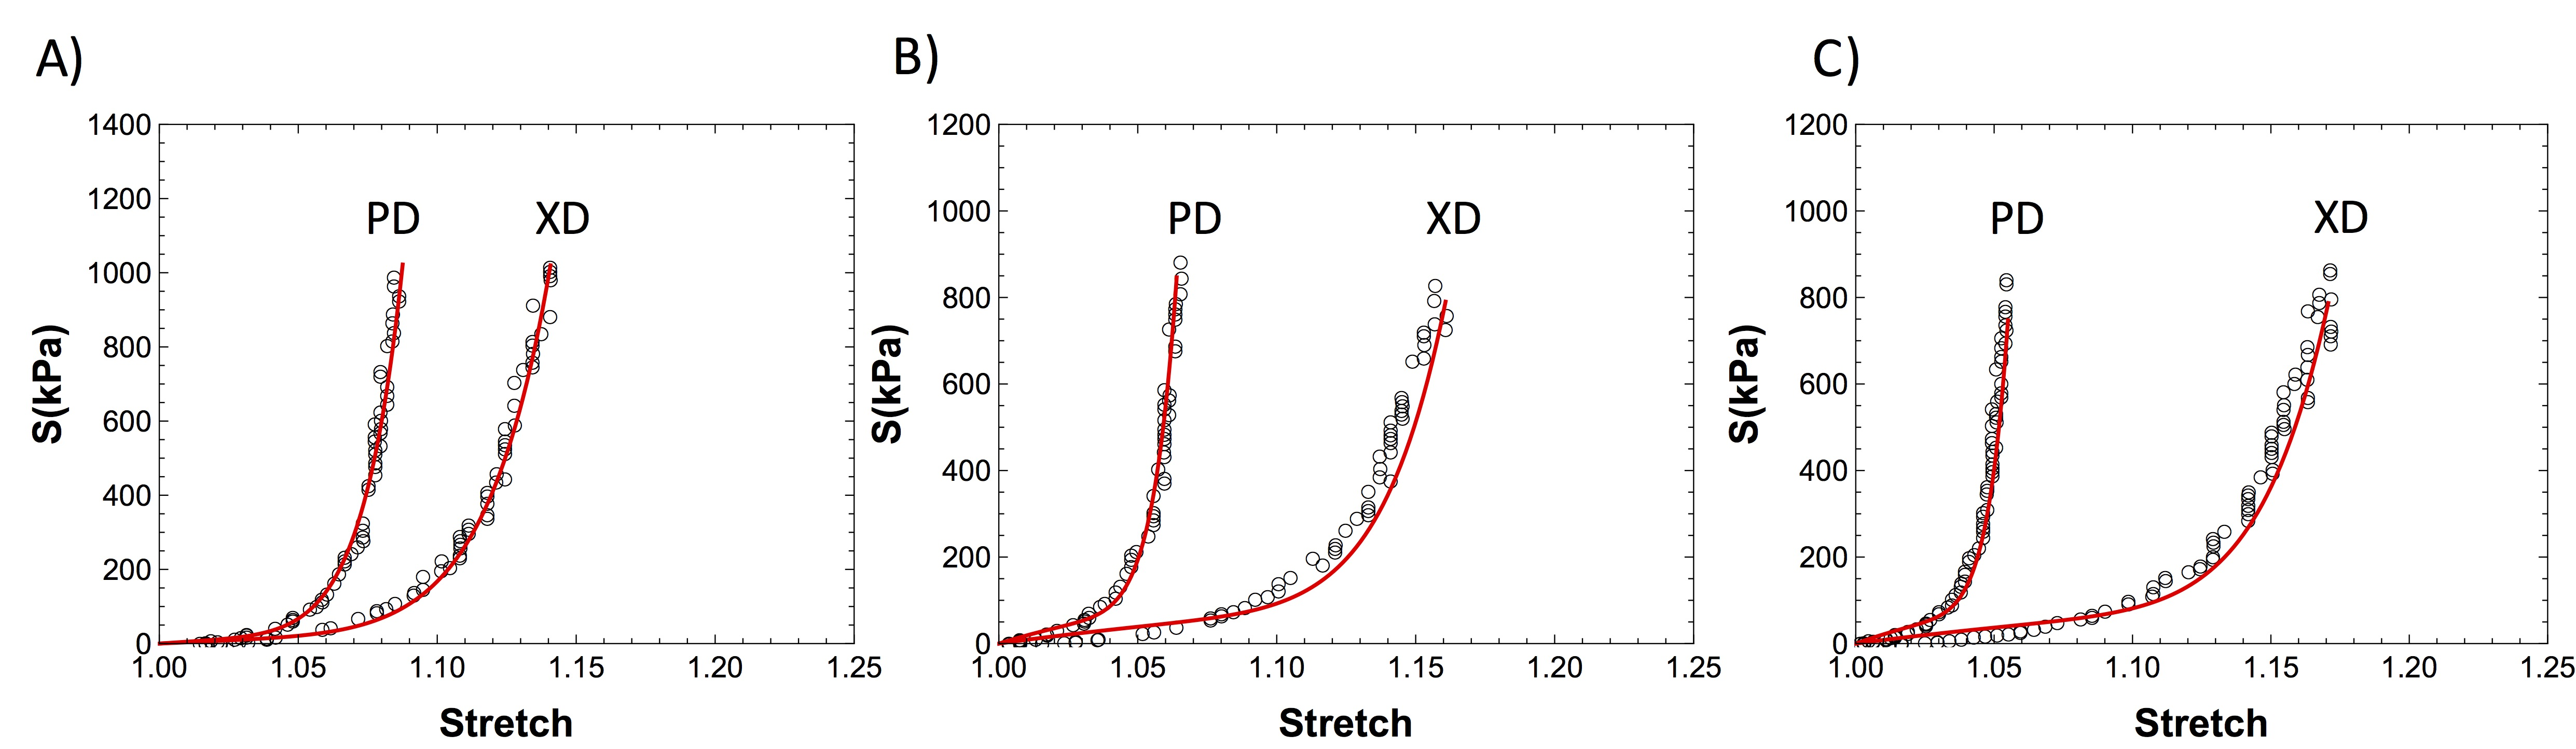
\includegraphics[width=0.35\paperwidth]{Images/chapter4/figure16}
\caption{The results of the parametric study. The red solid line shows the lower bound for the collagen fiber slack stretches and the red dashed line show the approximate cycle when the permanent set stretches reach an assymptote.}
\label{fig:parametric}
\end{figure}

%---    discussion
\section{Discussion}

\subsection{Permanent set is sufficient to describe early stages of BHV cycling}
	The most important result from this study is that permanent set alone is sufficient to explain all responses due to cyclic loading in the range of 0 to 65 million cycles. 
	This strongly suggests that there is no detectable damage to the collagen fiber architecture, and that the overall collagen fiber architecture stays intact and convected under affine kinematics. 
	This is not unexpected, as we previously found dense collagenous tissues to behave affinely when deforming in the physiological range \cite{lee_presence_2015}. 
	Although the permanent set effect is very noticeable in the early stages of the cyclic loading, it still takes millions of cycles; in other words, years. 
	Due to the time scale difference between the opening and closing of heart valves versus permanent set, BHVs always deforms quasi-statically, which means it always follows affine kinematics. 
	It follows that any structural changes in the collagen fiber architecture is affine as well. 
	This is all extremely important, as this allows us to completely separate permanent set from other cyclic loading effects and independently determine the permanent set rate constant just from the cyclic loading data in the early stage. 

\subsection{Lack of detectable structural damage}
	We observed in multiple instances \cite{sun_response_2004, sellaro_effects_2007} that there are molecular conformation changes in the collagen fiber during this early stage. 
	This suggests that while effects of collagen fiber damage are not detectable, it remains an ongoing but much slower process in comparison to permanent set. 
	Significant tearing and delamination are observed by Sacks and Smith \cite{sacks_effects_1998} after 500 million cycles, but this corresponds to the late stage of cyclic loading (Fig. \ref{fig:hypothesis}) during which we do not have extant mechanical data for constitutive modeling. 
	There are no other existing experimental data quantifying the intrinsic structural damage in BHVs during cyclic loading. 
	This is not surprising as actual structural damage is difficult to distinguish from other processes such as permanent set. 
	The relation between molecular changes and mechanical response is not well understood. 
	This requires multi-scale modeling for exogenously crosslinked tissue, which is also an extremely challenging task with no published studies currently. 
	The most promising way of quantifying structural damage is through constitutive modeling and simulations. 
	Structural models can separate structural damage and permanent set, but we do not have sufficiently data at high cycle numbers where structural damage is detectable. 
	This remains an important extension for the model in the future. 

\subsection{Permanent set is driven by the scission-healing of the matrix}
	One important assumption in our model is that permanent set only occurs in the matrix due to scission-healing. 
	Based on our theory for permanent set, the process is driven entirely by the first order kinetics of the crosslinking reactions of GLUT leading to scission-healing, as well as the kinematics involved in the reference state evolution. 
	Our results indicate that these mechanisms and permanent set can indeed explain the response to cyclic loading.
	This highlights the importance of understanding the effects of GLUT crosslinks and its role in the cyclic loading response of BHVs. 
	The use of GLUT was originally intended for suppressing immunogenicity by crosslinking antigen within BP xenographs, but also has the fortunate consequence of stiffening the mechanical response of the BHV. 
	Unfortunately, the scission-healing behavior of GLUT also playing a major role in the cyclic loading of BHVs. 
	By severely changing the geometry of the BHV in the first 1-2 years, it strongly influences the cyclic loading response of BHVs at latter stages. 
	It is difficult to properly design BHVs without accounting for the permanent set deformations caused by GLUT's scission-healing. 
	Alternative exogenous crosslinking chemistry \cite{tam_fixation_2017, tam_novel_2015} may be an important area for technological advancement of BHVs. 
	Protecting the optimal mechanical response of the BHVs by reducing the impact permanent set can significantly limit the peak stress on BHVs and protect the underlying tissue microstructure. 

\subsection{Recruitment of collagen fibers limit permanent set}
	Our parametric study of permanent set suggests that collagen fibers may play a significant role in limiting the effect of permanent set on the geometry of BHVs. 
	The stiffness of collagen fibers are over three magnitudes higher than the exogenously crosslinked matrix. 
	As collagen fibers are recruited, residual stress starts accumulating between collagen fibers and the matrix. 
	However, due to the significant difference in stiffness, the exogenously crosslinked matrix cannot extend the collagen fibers by a significant amount. 
	In addition, we generally found significant collagen fiber structural reserves in collagenous tissue \cite{zhang_meso_2016}. From the parametric study, no more than 2-4\% of collagen fibers are straightened under physiological loading levels (up to 1 MPa). 
	Also, taking into account the rapid recruitment of native collagen fibers (collagen fibers do not extend by more than 5-8\% strain before breaking \cite{buehler_atomistic_2006}), the collagen fiber architecture serves as a barrier in limiting the changes in geometry due to permanent set. 
	This potentially gives us a way of predicting and designing BHVs based on the expected maximum permanent set deformation. 

%---    discussion
%%%%%%%%%%%%%%%%%%%%%%%%%%%%%%%%%%%%%%%%%%%%%%%%%%%%%%%%%%%%%%%%%%%%%%%%%%%%%%%%
%%  Conclusions
%%%%%%%%%%%%%%%%%%%%%%%%%%%%%%%%%%%%%%%%%%%%%%%%%%%%%%%%%%%%%%%%%%%%%%%%%%%%%%%%


\section{Summary and Future Directions}
	We have developed the first structural-based constitutive model for the time evolving properties of exogenously crosslinked collagenous soft tissues under cyclic loading. We focused on permanent set as the mechanism for the geometry changes in the early stage of cycling and developed our constitutive model based on the underlying scission-healing reaction of the GLUT crosslinked matrix. Permanent set allows the reference configuration of the exogenously crosslinked matrix to evolve over time and convect the collagen fiber architecture through the change in geometry. The results show that permanent set alone is sufficient to explain all changes in the early stage of BHV cycling, and more importantly predict how the shape and reference configuration evolve during this stage. 	Moreover, structural damage does not play a detectable role up to 65 million cycles. Our model also indicates that the collagen fiber architecture can play a role in limiting the permanent set effect, where the straightening of collagen fibers prevents further changes in geometry. Thus, accounting for the permanent set effect is especially important in the design of BHVs to better improve their performance and durability. 
	
	In addition to the exogenously crosslinked tissue applications addressed herein, we have observed permanent set like phenomenon in mitral valve tissue during pregnancy \cite{rego_mitral_2016}. In that study, our results suggested that much of the growth and remodeling in the MV leaflet does not begin immediately, but rather undergoes mostly passive leaflet enlargement until these parameters reach a critically low level, at which point growth and remodeling are triggered. This initial tissue distension process is very similar in behavior to the permanent set mechanism outlined in the present work. Thus, the current approach could be applied to these types of the early phases soft tissue remodeling, where non-failure mechanisms occur before the onset of growth of tissue growth and remodeling. In addition, although the permanent set model we described only include the remodeling of the matrix due to scission-healing, the same concept can be extended by separating the rate constant into growth and resorption to simulate growth and remodeling of the matrix. Furthermore, the frame work outlined in section 5 can also be extended for the remodeling of the collagen fiber architecture, given further studies on mechanisms for how the collagen fiber architecture grows once the critical level observed in Rego \textit{et al} \cite{rego_mitral_2016} is exceeded. This is the advantage for the structural-based approach to modeling permanent set, which allows us to describe the mechanical response based on real physically measure-able quantities. We can further extend the more toward effects such as structural damage are the fiber-level, proteolytic degradation, and growth based on how this effects affect the components of the permanent set model layed out herein.


%%%%%%%%%%%%%%%%%%%%%%%%%%%%%%%%%%%%%%%%%%%%%%%%%%%%%%%%%%%%%
%%  nomenclature											%
%%%%%%%%%%%%%%%%%%%%%%%%%%%%%%%%%%%%%%%%%%%%%%%%%%%%%%%%%%%%%
\section*{Nomenclature} \label{c4:sec:nomenclature}
\begin{mynom}
\textbf{Key Terms}   \\
{Matrix}\>\>\tabfill{Non-fibrous part of the extracellular matrix }  \\
{EXL}\>\tabfill{Exogenously crosslinked}  \\
{PS}\>\tabfill{Permanent set, an irreversible deformation that remains in a structure or material after it has been subjected to stress.}  \\
{Damage}\>\>\tabfill{Loss of mechanical properties}  \\
{Fatigue}\>\>\tabfill{Weakening of a material caused by repeated loading}  \\
{Plastic deformation}\>\>\>\>\>\tabfill{Deformation of a material undergoing irreversible change in shape in response to applied forces}  \\
{Structural convection}\>\>\>\>\>\>\tabfill{A permanent deformation of the collagen fiber architecture based on the change in the reference configuration}  \\
{BP}\>\tabfill{Bovine pericardium}  \\
{CFA}\>\tabfill{Collagen fiber architecture}  \\
{BHV}\>\tabfill{Bioprosthetic heart valve}  \\
{AWT}\>\tabfill{Accelerated wear testing}  \\
{GLUT}\>\tabfill{Glutaraldehyde}  \\
{TVI}\>\tabfill{Transcatheter aortic intervention }  \\
{PD}\>\tabfill{Preferred direction}  \\
{XD}\>\tabfill{Cross-preferred direction}  \\
{ODF}\>\tabfill{Orientation distribution function}  \\
{Recruitment}\>\>\>\tabfill{Probability distribution function describing the strain at which a collagen fiber's crimp is straightened }  \\ 
{Fiber ensemble}\>\>\>\>\tabfill{A group of fibers which share a common orientation}  \\
\textbf{Symbols}      \\
{$\Psi$}\>\tabfill{Strain energy}  \\
{$\Psi_\mathrm{col}, \Psi_\mathrm{int}, \Psi_m$}\>\>\>\tabfill{Strain energy of the collagen fiber, ensemble-ensemble interactons, and matrix components respectively}  \\
{$D$}\>\tabfill{Collagen fiber recruitment distribution function}  \\
{$\lambda_s$}\>\tabfill{The slack stretch, the stretch needed to straighten the collagen fiber crimp }  \\
{$\Gamma$}\>\tabfill{Collagen fiber orientation distribution function}  \\
{$\phi$}\>\tabfill{Mass fraction}  \\
{$\eta_C$, $\eta_m$, $\eta_I$}\>\>\>\tabfill{The modulus of collagen, EXL matrix and fiber-fiber interactions}  \\
{$\mathbf{I}$}\>\tabfill{Identity tensor}  \\
{$\mathbf{F}$}\>\tabfill{An arbitrary deformation gradient tensor applied to the tissue, referenced to the original uncycled stress free state}  \\
{$\mathbf{C}$}\>\tabfill{Right Cauchy-Green strain tensor, referenced to the original uncycled stress free state}  \\
{$\mathbf{E}$}\>\tabfill{Green Lagrange strain, referenced to the original uncycled stress free state}  \\
{$\lambda$}\>\tabfill{Stretch}  \\
{$\mathbf{n}_\alpha$}\>\tabfill{A vector pointing at the angle $\alpha$ }  \\
{$\lambda_\alpha = \sqrt{\mathbf{n}_\alpha \cdot \mathbf{C} \mathbf{n}_\alpha}$}\>\>\>\>\tabfill{The applied stretch at the fiber ensemble-level in the direction $\alpha$ }  \\
{$\prescript{}{\alpha}{\lambda}_s$}\>\tabfill{The slack stretch of a collagen fiber oriented with the angle $\alpha$ }  \\
{$\mathbf{S}$}\>\tabfill{Second Piola Kirchhoff tensor, referenced to the original uncycled stress free state}  \\
{$I_1$}\>\tabfill{First invariant}  \\
{$I_8$}\>\tabfill{Eighth pseudo invariant}  \\
{$I_8^rot$}\>\tabfill{The rotational component of $I_8$ }  \\
{$I_8^ext$}\>\tabfill{The extensional component of $I_8$ }  \\
{$k$}\>\tabfill{Rate constant for permanent set}  \\
{$s$}\>\tabfill{The current time in seconds }  \\
{$\hat{s}$}\>\tabfill{The intermediate time when the EXL matrix is formed by the scission-healing process }  \\
{$\Omega_0$}\>\tabfill{The original unloaded configuration of the tissue before any cyclic loading}  \\
{$\Omega(s)$}\>\tabfill{The current loaded configuration of the tissue during cyclic loading}  \\
{$\mathbf{A}(s)$}\>\tabfill{Strain history, which is the root mean square strain of each cycle as a function of time}  \\
{$\mathbf{\tilde{B}}(s) = \mathbf{A}\mathbf{A}^\mathsf{T}$}\>\>\>\tabfill{Left Cauchy Green tensor of the strain history}  \\
{$\mathbf{\bar{F}}(\hat{s})$}\>\tabfill{Deformation gradient tensor applied to the tissue, referenced to the strain history $\mathbf{A}(\hat{s})$ at time $\hat{s}$}  \\
{$\mathbf{\bar{C}}(\hat{s})$}\>\tabfill{The right Cauchy Green strain tensor applied to the tissue, referenced to the strain history $\mathbf{A}(\hat{s})$ at time $\hat{s}$}  \\
{$\bar{I}_1$}\>\tabfill{Modified first invariant, referenced to the strain history $\mathbf{A}(\hat{s})$ at time $\hat{s}$}  \\
{$\bar{\mathbf{\Psi}}_m$}\>\tabfill{Strain energy of the matrix as function of $\bar{I}_1$}  \\
{$\bar{\mathbf{S}}_m$}\>\tabfill{Stress of the matrix as function of $\bar{I}_1$}  \\
{$\Omega_\mathrm{PS}(s)$}\>\tabfill{The current unloaded configuration due to changes in geometry caused by permanent set}  \\
{$\mathbf{F}_\mathrm{PS}(s)$}\>\tabfill{The deformation from $\Omega_0$ to the current unloaded configuration ($\Omega_\mathrm{PS}$) due to permanent set}  \\
{$b(s)$}\>\tabfill{The proportion of the existing amount of material remaining}  \\
{$a(s,\hat{s})$}\>\tabfill{The proportion of the material newly formed at time $\hat{s}$ remaining}  \\
{$\prescript{1}{0}{\mathbf{F}}$}\>\tabfill{The deformation gradient from $\Omega_0$ to some arbitrary state $\Omega_1$, most commonly $\Omega_1 = \Omega_\mathrm{PS}$ }  \\
{$\prescript{1}{0}{\lambda}(\theta_0)$}\>\tabfill{The stretch of an ensemble oriented along $\theta_0$ in $\Omega_0$ deformed from $\Omega_0$ to some arbitrary state $\Omega_1$}  \\
{$D_1$}\>\tabfill{The collagen fiber recruitment distribution function convected from $\Omega_0$ to to some arbitrary state $\Omega_1$ }  \\
{$\Gamma_1$}\>\tabfill{The collagen fiber orientation distribution function convected from $\Omega_0$ to to some arbitrary state $\Omega_1$}  \\
{$\mathbf{\hat{S}}$}\>\tabfill{The applied stress during cyclic loading }  \\
\end{mynom}


%---    Bioliography
\bibliographystyle{plainnat}
\bibliography{phd}

